%%%%%%%%%%%%%%%%%%%%%%% file template.tex %%%%%%%%%%%%%%%%%%%%%%%%%
%
% This is a general template file for the LaTeX package SVJour3
% for Springer journals.          Springer Heidelberg 2010/09/16
%
% Copy it to a new file with a new name and use it as the basis
% for your article. Delete % signs as needed.
%
% This template includes a few options for different layouts and
% content for various journals. Please consult a previous issue of
% your journal as needed.
%
%%%%%%%%%%%%%%%%%%%%%%%%%%%%%%%%%%%%%%%%%%%%%%%%%%%%%%%%%%%%%%%%%%%
%
% First comes an example EPS file -- just ignore it and
% proceed on the \documentclass line
% your LaTeX will extract the file if required
\begin{filecontents*}{example.eps}
%!PS-Adobe-3.0 EPSF-3.0
%%BoundingBox: 19 19 221 221
%%CreationDate: Mon Sep 29 1997
%%Creator: programmed by hand (JK)
%%EndComments
gsave
newpath
  20 20 moveto
  20 220 lineto
  220 220 lineto
  220 20 lineto
closepath
2 setlinewidth
gsave
  .4 setgray fill
grestore
stroke
grestore
\end{filecontents*}
%
\RequirePackage{fix-cm}
%
%\documentclass{svjour3}                     % onecolumn (standard format)
%\documentclass[smallcondensed]{svjour3}     % onecolumn (ditto)
\documentclass[smallextended]{svjour3}       % onecolumn (second format)
%\documentclass[twocolumn]{svjour3}          % twocolumn
%
\smartqed  % flush right qed marks, e.g. at end of proof
%
\usepackage{todonotes}
\usepackage{graphicx}
\usepackage{multirow}
\usepackage{amsmath}
\usepackage{amsfonts}
\usepackage{amssymb}
\usepackage{graphicx}
\usepackage[round]{natbib}
\usepackage{url}
%\usepackage{subfigure}
\usepackage{epstopdf}
\setcounter{MaxMatrixCols}{30}
%\usepackage{algorithm}
%\usepackage{algorithmic}
\usepackage{subfigure}
\usepackage{xcolor}
\newcommand{\highlight}[1]{%
  \colorbox{gray!50}{$\displaystyle#1$}}
%\usepackage{subcaption}
\usepackage{fancyhdr}
\usepackage{booktabs}
\graphicspath{{../}{figures/}}
%\usepackage{todonotes}
 
%\usepackage{subcaption}

%\usepackage{cleveref}
%
% \usepackage{mathptmx}      % use Times fonts if available on your TeX system
%
% insert here the call for the packages your document requires
%\usepackage{latexsym}
% etc.
%
% please place your own definitions here and don't use \def but
% \newcommand{}{}
%
% Insert the name of "your journal" with
\journalname{dataminingknowledgediscovery}
%
%\usepackage{subfigure}
%%Preamble File for Random Regression Paper

%\usepackage{times}

%Theorems and such

%\usepackage{amsthm}

%\newtheorem{theorem}{Theorem}
%\newtheorem{observation}{Observation}
%\newtheorem{proposition}{Proposition}
%\newtheorem{definition}{Definition}

%\newtheorem{theorem}{Theorem}[section]
%\newtheorem{observation}{Observation}[section]
%\newtheorem{proposition}{Proposition}[section]
%\newtheorem{definition}{Definition}[section]

\usepackage[ruled,vlined]{algorithm2e}
\usepackage{algorithmic}
%\usepackage{amsthm}
\usepackage{amsmath}
\usepackage{amsfonts}
\usepackage{amssymb}
\usepackage{graphicx}
\usepackage{url}
\usepackage{subfigure}
\usepackage{epstopdf}
%\setcounter{MaxMatrixCols}{30}
%\usepackage[ruled,vlined]{algorithm2e}
%\usepackage{algorithmic}
\usepackage{multirow}
\usepackage{subfigure}
\usepackage{ifthen}
\DeclareMathOperator*{\argmax}{argmax}
\DeclareMathOperator*{\argmin}{argmin}
%\DeclareMathOperator{\pattern}{\pi}
\DeclareMathOperator{\Poly}{\mathbf{\mathrm{P}}}
\DeclareMathOperator{\RP}{\mathbf{\mathrm{RP}}}
%\DeclareMathOperator{\FP}{\mathbf{\mathrm{FP}}}
\DeclareMathOperator{\NP}{\mathbf{\mathrm{NP}}}
%\DeclareMathOperator{\E}{\mathbb{E}}

\newcommand{\defterm}{\textbf}

\renewcommand{\d}{\mathbf{d}}

\newcommand{\ZZ}{\mathbf{Z}}

\newcommand{\indep}{\ensuremath{\perp{}\!\!\!\!\!\!\!\perp{}}}
\newcommand{\dep}{\ensuremath{{\perp{}\!\!\!\!\!\!\!\not  \perp{}}}}
%\renewcommand{\L}{\mathcal{L}}

% variables denoting sets of nodes
\newcommand{\BN}{B} % Bayes net
\newcommand{\V}{V} 
\newcommand{\partC}{\mathcal{C}}
\newcommand{\pattern}{\pi}
% for population variables
\newcommand{\A}{\mathbb{A}}
\newcommand{\B}{\mathbb{B}}
\newcommand{\C}{\mathbb{C}}
\newcommand{\U}{\mathbb{U}}
%maybe use P, R as well??
\renewcommand{\P}{P}
\newcommand{\R}{R}
% values of Pop variables = constants
\renewcommand{\a}{a}
\renewcommand{\b}{b}
\renewcommand{\c}{c}

%%%
% for terms = nodes in Functor Bayes Net.
\newcommand{\X}{X}
\newcommand{\Y}{Y}
\newcommand{\Z}{Z}
% Next three are currently only ones eligible for \Mrange and \Prange
\newcommand{\TT}{T}
\newcommand{\TI}{\mathsf{T}}
\newcommand{\UT}{U}
\newcommand{\UI}{\mathsf{U}}
\newcommand{\VT}{V}
\newcommand{\VI}{\mathsf{V}}
\newcommand{\W}{W}
%syntax for values
\newcommand{\z}{z}
\renewcommand{\v}{v}
\newcommand{\x}{x}
\newcommand{\y}{y}
\newcommand{\p}{p}
\newcommand{\s}{s}
% Values tied to terms
\newcommand{\TV}{t}
\newcommand{\TTuple}[1][0.0ex]{\vec{t}\hspace{#1}}
\newcommand{\UV}{u}
\newcommand{\UTuple}[1][0.0ex]{\vec{u}\hspace{#1}}
\newcommand{\VV}{v}
\newcommand{\VTuple}{\vec{v}}
%%%
\newcommand{\weight}{w} % weights
% Formulas
\newcommand{\TF}{\vec{T}}
\newcommand{\UF}{\vec{U}}
\newcommand{\VF}{\vec{V}}
%\newcommand{\TF}{\phi}
%\newcommand{\UF}{\psi}
%\newcommand{\VF}{\omega}
% Database (which is always fully-grounded)
\newcommand{\DB}{\FG{\Delta}}
\newcommand{\QC}{\FG{\Lambda}}
\newcommand{\QCtarget}{\FG{\Lambda_{-\TI}}}
% to define a query conjunction of literals
\newcommand{\Qconj}{\Appendterm{\FG{\TT_{\grounding}} = \TV} {\QC}}

% Annotations marking degree of grounding
\newcommand{\UG}[2][0.0ex]{#2^{-}\hspace{#1}}
\newcommand{\PG}[2][0.0ex]{#2^{\prime}\hspace{#1}}
\newcommand{\FG}[2][0.0ex]{#2^{*}\hspace{#1}}

% Functions returning related terms
\newcommand{\MB}[1]{\mathrm{MB}(#1)}
\newcommand{\Pa}[1]{\mathrm{Pa}(#1)}
\newcommand{\Ch}[1]{\mathrm{Ch}(#1)}

% Grounding
\newcommand{\Ground}[1]{#1_\gamma}
\newcommand{\gndlink}{\backslash}

% Values in ranges of example functors
\newcommand{\Man}{\mathrm{M}}
\newcommand{\Woman}{\mathrm{W}}

% Adding a term to a formula
\newcommand{\sepcup}[1][0.5ex]{\hspace{#1}\cup\hspace{#1}}
\newcommand{\Setaddterm}[2]{#1 \sepcup #2}
\newcommand{\Appendterm}[2]{#1, #2}

% Values in the range of related terms
\newcommand{\Mrange}[1]{\ifthenelse{\equal{#1}{T}}{\TTuple_m}{\ifthenelse{\equal{#1}{U}}{\UTuple_m}{\ifthenelse{\equal{#1}{V}}{\VTuple_m}{\mbox{UNKNOWN
TERM ID}}}}}
\newcommand{\Prange}[1]{\ifthenelse{\equal{#1}{T}}{\vec{t}_{pa}}{\ifthenelse{\equal{#1}{U}}{\vec{u}_{pa}}{\ifthenelse{\equal{#1}{V}}{\vec{v}_{pa}}{\mbox{UNKNOWN
TERM ID}}}}}

\newcommand{\GroundPrange}[1]{\ifthenelse{\equal{#1}{T}}{\vec{t}_{pa,\grounding'}}{\ifthenelse{\equal{#1}{U}}{\vec{u}_{pa,\grounding'}}{\ifthenelse{\equal{#1}{V}}{\vec{v}_{pa,\grounding'}}{\mbox{UNKNOWN
TERM ID}}}}}


% Key functions
\newcommand{\joint}{p}
\newcommand{\jprob}[1]{\theta(#1)}
\newcommand{\cprob}[2]{\theta(#1|#2)}
\newcommand{\estcprob}[3]{\widehat{\theta}(#1|#2;#3)}
%\newcommand{\Gpvar}{\tilde{P}}
\newcommand{\Gpvar}{P}
\newcommand{\Gprob}[2]{\Gpvar(#1 | #2)}
\newcommand{\QFC}{QFC} % query family configuration
\newcommand{\Cvar}{\mathrm{n}}
\newcommand{\Fvar}{\mathrm{p}}
\newcommand{\Count}[2]{\Cvar\left[#1;#2\right]}
\newcommand{\CountC}[3]{\Cvar_{#3}\left[#1;#2\right]}
\newcommand{\Freq}[2]{\Fvar\left[#1;#2\right]}
\newcommand{\Relevant}[1]{#1^{\mathrm{r}}}
\newcommand{\Relcount}[2]{\Relevant{\Cvar}\left[#1;#2\right]}
\newcommand{\RelcountC}[3]{\Relevant{\Cvar_{#3}}\left[#1;#2\right]}
\newcommand{\Relfreq}[2]{\Relevant{\Fvar}\left[#1;#2\right]}
\newcommand{\RelfreqC}[3]{\Relevant{\Fvar_{#3}}\left[#1;#2\right]}
\newcommand{\Range}[1]{\mathrm{Ra}(#1)}
\newcommand{\Vars}[1]{\mathrm{Va}(#1)}
% no longer needed
%\newcommand{\Crossprod}[1]{\mathcal{X}}

%variables for sets of values
\newcommand{\setx}{\set{x}}
\newcommand{\sety}{\set{y}}
\newcommand{\setz}{\set{z}}


%statistics
\newcommand{\score}{S}
\newcommand{\parameters}{\mathit{par}}
\newcommand{\bic}{\mathit{BIC}}
%random variables and graphical models
% number of values in the domain of a random variable
% variables for BNs
\newcommand{\domvals}{k}
\newcommand{\nodevalue}{\x}
\newcommand{\parvalue}{\mathbf{\pi}} % a single assignment of values to a set of 
%parents
\newcommand{\parvals}{l} % number of values of parent state.
\renewcommand{\r}{r} % CP-table row
\newcommand{\nbhd}{{\mathsf {nbdh}}}
\newcommand{\child}{\mathit{child}}
\newcommand{\parent}{\mathit{pa}}
\newcommand{\parents}{\mathbf{pa}}
\newcommand{\Parents}{\mathbf{PA}}
\newcommand{\family}{F} % families, family formulas
\newcommand{\Target}{Y_{\target}}
\newcommand{\MBtarget}{\set{X}_{\target}} % Markov blanket of a target node.
\newcommand{\mbtarget}{\set{x}} % values for the markov blanket of a variable, vector-valued
\newcommand{\mbstates}{m} % number of states in Markov blanket
\newcommand{\vpi}{\mathbf{pa}} % for vectors of variable assignments
\renewcommand{\l}{\ell} % class label
\newcommand{\states}{r} % number of states of a variable
\newcommand{\ssize}{N} % number of rows in join table; size of sample
\newcommand{\frequency}{fr}
\newcommand{\pseudo}{\ast}
\newcommand{\counts}{+}
\newcommand{\weighted}{\ast}
\newcommand{\halpern}{H}
\newcommand{\instance}{I}

%logic notation
\newcommand{\functor}{f}
\newcommand{\fvalue}{v}
\newcommand{\variable}{X} % first-order variable
\newcommand{\population}{\mathcal{P}}
\newcommand{\entity}{x}
\newcommand{\formula}{\phi}
\newcommand{\formulas}{\mathcal{\phi}}
\newcommand{\conjunction}{\set{C}} % 
\newcommand{\outdomain}{V}
\newcommand{\literal}{\ell}
%conjunction of literals
\newcommand{\fterm}{\f} % open function term
\newcommand{\fterms}{F} % set of function terms, also nodes in JBN
\newcommand{\term}{\tau}
\newcommand{\terms}{\bs{\tau}}
\newcommand{\constant}{a}
\newcommand{\constants}{\bs{\constant}}
\newcommand{\gterm}{g} % ground term
\newcommand{\gterms}{\bs{\gterm}} %list of ground terms
\newcommand{\vterm}{x} % variable term
\newcommand{\vterms}{\bs{\vterm}} % list of variable terms
\newcommand{\assign}{A} % assignment of values to Bayes net
\newcommand{\grounds}{\#}
\newcommand{\grounding}{\gamma}
\newcommand{\groundall}{\Gamma}
\newcommand{\vars}{\mathit{Var}} % variables in a conjunction
\newcommand{\igraph}{I} % instance-level dependency graph.
\newcommand{\assignment}{\set{a}}
\newcommand{\atom}{\functor}
\newcommand{\gnode}{\alpha}
\newcommand{\gfamily}{\ground{f}}
\newcommand{\numformulas}{m}
% logic programs
\newcommand{\program}{\mathcal{B}}
\newcommand{\clause}{\mathcal{c}}
\newcommand{\head}{\mathit{head}}
\newcommand{\body}{\mathit{body}}
\newcommand{\crule}{\mathit{cr}} % combining rule
\newcommand{\level}{\mathit{level}} % rank of function symbols in LP

%datbase schema
\newcommand{\rcolumns}{R}
\newcommand{\ecolumns}{E}
\newcommand{\dtable}{T} % can't use \table. Generic database table
\newcommand{\datatable}{D} % generic data table, not necessarily part of database.
\newcommand{\jtable}{J} % join table
\newcommand{\Ejoin}{$J^{+}$}
\newcommand{\jtables}{m}
\newcommand{\rtable}{R} % relationship table
\newcommand{\etable}{E} % entity table.
\newcommand{\ttable}{X} % target table
\newcommand{\nextended}{n}
\newcommand{\row}{r}
\newcommand{\rows}{\mathit{rows}}
\newcommand{\col}{j}
\newcommand{\cols}{\mathit{cols}}
\newcommand{\unary}{\f} % to denote a unary or attribute function
\newcommand{\numatts}{u} % to denote the number of unary or attribute functions.
\newcommand{\g}{g} % alternative for function
\newcommand{\relational}{\mathbf{r}} % denotes a generic relational functors, can be both relationship or descriptive attribute of relationship
\newcommand{\Relation}{R} % denotes a generic boolean relation
% a special type of literal conjunction that assigns a value %to each variable
\newcommand{\class}{c} % the class attribute
\newcommand{\classifier}{\mathcal{C}}
\newcommand{\target}{t} % target object
\newcommand{\feature}{f} % feature or desc attribute of object or link
\newcommand{\features}{\bs{f}} % features 
\newcommand{\attribute}{a} % nonclass attribute of target object
\newcommand{\attributes}{\bs{a}}
\newcommand{\rels}{\bs{R}} % chain of relationships.
\newcommand{\maxpath}{\rho}

%special functions
\newcommand{\AVG}{\it{AVG}}
\newcommand{\instances}{n} % counts number of occurrences in DB
\newcommand{\prob}{p} % frequency of formula true in in DB

%variables denoting graphs or models
\newcommand{\mln}{M}
\newcommand{\G}{G}
\newcommand{\node}{X}
\newcommand{\nodes}{V}
\newcommand{\edges}{E}
\newcommand{\clique}{C}
\newcommand{\cliques}{\mathcal{\clique}}
\newcommand{\cliquevalue}{c}
\newcommand{\graph}{G}
\newcommand{\M}{M}
\newcommand{\J}{J}
\renewcommand{\H}{H}
\newcommand{\K}{K} % component
\renewcommand{\O}{O} % oracle
\renewcommand{\path}{\rho} % path, also foreignkey path
% Markov nets
\newcommand{\potential}{\Psi}
% database schema
\newcommand{\type}{\tau} % to denote a generic type
\newcommand{\E}{E} % for entity tables
\newcommand{\e}{e} % for specific entities
\newcommand{\f}{f}
\newcommand{\new}{\it{new}}
\renewcommand{\c}{c}
\renewcommand{\R}{R} % for relationship tables
%\newcommand{\A}{A} % for attributes
\newcommand{\T}{T} % for tables generically
\newcommand{\New}{N}
\newcommand{\D}{\mathcal{D}} % for database instance
\renewcommand{\S}{\mathcal{S}} % for relational structure as conjunction of literals
\newcommand{\databases}{\set{D}} % the number of databases
\newcommand{\vocab}{\mathcal{\L}} % for logical vocabulary associated with database
\newcommand{\name}{\mathit{name}} % generic attribute
\newcommand{\dom}{\mathit{dom}} % domain of attributes
\newcommand{\etables}{\alpha} % entity tables
\newcommand{\rtables}{\beta} % relationship table number
% specific constructs for examples
\newcommand{\student}{\mathit{Student}}
\newcommand{\I}{\mathit{I}}
\newcommand{\course}{C}
\newcommand{\prof}{\mathit{Professor}}
\newcommand{\person}{\mathit{Person}}
\newcommand{\TA}{\mathit{TA}}
\newcommand{\actor}{\mathit{Actor}}
\newcommand{\age}{\mathit{age}}
\newcommand{\intelligence}{\mathit{intelligence}}
\newcommand{\diff}{\mathit{difficulty}}
\newcommand{\reg}{\mathit{Registered}}
\newcommand{\ra}{\mathit{RA}}
\newcommand{\bt}{\mathit{blood type}}
\newcommand{\grade}{\mathit{grade}}
\newcommand{\gpa}{\mathit{gpa}}
\newcommand{\jack}{\mathit{Jack}}
\newcommand{\jill}{\mathit{Jill}}
\newcommand{\smith}{\mathit{Smith}}
\newcommand{\cmpt}{\mathit{CMPT120}}
\newcommand{\hi}{\mathit{Hi}}
% various constants
\newcommand{\true}{\mathrm{T}}
\newcommand{\false}{\mathrm{F}}
\newcommand{\normalconstant}{Z} % the normalization constant

% orderings
\newcommand{\pred}{\mathit{pred}}
%procedure names and such
\newcommand{\join}{\textsc{Join-Frequencies}}
\newcommand{\linus}{\textsc{Linus }}
\newcommand{\foil}{\textsc{Foil }}
\newcommand{\MLN}{\textsc{MLN}}
\newcommand{\treetilde}{\textsc{TILDE }}

%%%
%undirected models
\newcommand{\pot}{\phi} % potential function
%\newcommand{\theHalgorithm}{\arabic{algorithm}}
\newcommand{\test}{test}
\def\set#1{\mathbf{#1}}
\def\bs#1{\boldsymbol{#1}}
\def\ground#1{\overline{#1}}

\DeclareMathOperator*{\argmax}{argmax}
\DeclareMathOperator*{\argmin}{argmin}
%\DeclareMathOperator{\pattern}{\pi}
\DeclareMathOperator{\Poly}{\mathbf{\mathrm{P}}}
\DeclareMathOperator{\RP}{\mathbf{\mathrm{RP}}}
%\DeclareMathOperator{\FP}{\mathbf{\mathrm{FP}}}
\DeclareMathOperator{\NP}{\mathbf{\mathrm{NP}}}
%\DeclareMathOperator{\E}{\mathbb{E}}
\renewcommand{\d}{\mathbf{d}}

\newcommand{\ZZ}{\mathbf{Z}}

\newcommand{\indep}{\ensuremath{\perp{}\!\!\!\!\!\!\!\perp{}}}
\newcommand{\dep}{\ensuremath{{\perp{}\!\!\!\!\!\!\!\not  \perp{}}}}
%\renewcommand{\L}{\mathcal{L}}
% variables denoting sets of nodes
\newcommand{\V}{V} 
\newcommand{\partC}{\mathcal{C}}
\newcommand{\pattern}{\pi}
% variables denoting nodes
\newcommand{\B}{B}
\renewcommand{\P}{P}
\newcommand{\R}{R}
\newcommand{\X}{X}
\newcommand{\Y}{Y}
\newcommand{\Z}{Z}
\newcommand{\F}{F}
\newcommand{\U}{U}
\newcommand{\W}{W}
\renewcommand{\S}{S}
\newcommand{\C}{C}
\newtheorem{mydef}{Proposition}
%variables for values
%\newcommand{\u}{u}
\renewcommand{\a}{a}
\renewcommand{\b}{b}
\newcommand{\z}{z}
\renewcommand{\v}{v}
\newcommand{\x}{x}
\newcommand{\y}{y}
\newcommand{\p}{p}
\newcommand{\s}{s}
\newcommand{\w}{w} % weights
\newcommand{\TVD}{TVD}

%statistics
\newcommand{\divergence}{\it{D}}
\newcommand{\score}{\it{score}}
\newcommand{\confidence}{\it{conf}}
\newcommand{\support}{\it{support}}
\newcommand{\loglikelihood}{\it{LOG}}
\newcommand{\lof}{\it{LOF}}
\newcommand{\llmetric}{-L}
\newcommand{\lr}{\it{LR}}
\newcommand{\kl}{\it{KL}}
\newcommand{\el}{\it{EL}}
\newcommand{\mi}{\it{MI}}
\renewcommand{\mid}{\it{ELD}}
\newcommand{\jid}{\it{JID}}
\newcommand{\roc}{\it{ROC}}
\newcommand{\outrank}{\it{OutRank}}
\newcommand{\knn}{\it{KNNOutlier}}
\newcommand{\auc}{\it{AUC}}
\newcommand{\eld}{\it{ELD}}
\newcommand{\fd}{\it{FD}}
\newcommand{\parameter}{\theta}
\newcommand{\parameters}{\bs{\parameter}}
\newcommand{\bic}{\mathit{BIC}}
%random variables and graphical models
% number of values in the domain of a random variable
% variables for BNs
\newcommand{\domvals}{k}
\newcommand{\nodevalue}{\v}
\newcommand{\parvalue}{\mathbf{\pi}} % a single assignment of values to a set of 
%parents
\newcommand{\parvals}{l} % number of values of parent state.
\renewcommand{\r}{r} % CP-table row
\newcommand{\nbhd}{{\mathsf {nbdh}}}
\newcommand{\child}{\mathit{child}}
\newcommand{\parent}{\mathit{pa}}
\newcommand{\parents}{\mathbf{pa}}
\newcommand{\Parents}{\mathbf{PA}}
\newcommand{\family}{F} % families, family formulas
\newcommand{\vpi}{\mathbf{pa}} % for vectors of variable assignments
\renewcommand{\l}{\ell} % class label
\newcommand{\states}{r} % number of states of a variable
%\newcommand{\value}{value}
\newcommand{\mb}{\set{mb}} % markov blanket of a variable, vector-valued
\newcommand{\ssize}{N} % number of rows in join table; size of sample
\newcommand{\mbstates}{m} % number of states in Markov blanket
\newcommand{\frequency}{fr}
\newcommand{\pseudo}{\ast}
\newcommand{\counts}{+}
\newcommand{\weighted}{\ast}
\newcommand{\halpern}{H}
\newcommand{\Thetaa}{\theta}
\newcommand{\instance}{I}

%logic notation
%\newcommand{\predicate}{\phi}
\newcommand{\functor}{f}
\newcommand{\outdomain}{V}
\newcommand{\indomain}{\Omega}
\newcommand{\variable}{X} % first-order variable
\newcommand{\population}{\mathcal{P}}
\newcommand{\entity}{x}
\newcommand{\formula}{\phi}
\newcommand{\formulas}{\mathcal{\phi}}
\newcommand{\literal}{l}
\newcommand{\conjunction}{\set{C}} % conjunction of literals
\newcommand{\fterm}{\f} % open function term
\newcommand{\fterms}{F} % set of function terms, also nodes in JBN
\newcommand{\term}{\sigma}
\newcommand{\Terms}{\bs{\sigma}}
\newcommand{\constant}{a}
\newcommand{\constants}{\bs{\constant}}
\newcommand{\gterm}{g} % ground term
\newcommand{\gterms}{\bs{\gterm}} %list of ground terms
\newcommand{\vterm}{x} % variable term
\newcommand{\vterms}{\bs{\vterm}} % list of variable terms
\newcommand{\assign}{A} % assignment of values to Bayes net
\newcommand{\resultset}{\mathbb{R}}
\newcommand{\grounds}{\#}
\newcommand{\grounding}{\gamma}

\newcommand{\vars}{\mathit{Var}} % variables in a conjunction
\newcommand{\igraph}{I} % instance-level dependency graph.
\newcommand{\assignment}{\set{a}}
\newcommand{\atom}{\ell}
\newcommand{\gnode}{\alpha}
\newcommand{\gfamily}{\ground{f}}
\newcommand{\numformulas}{m}
\newcommand{\structure}{\mathcal{S}}
% logic programs
\newcommand{\program}{\mathcal{B}}
\newcommand{\clause}{\mathcal{c}}
\newcommand{\head}{\mathit{head}}
\newcommand{\body}{\mathit{body}}
\newcommand{\crule}{\mathit{cr}} % combining rule
\newcommand{\level}{\mathit{level}} % rank of function symbols in LP

%datbase schema
\newcommand{\rcolumns}{R}
\newcommand{\ecolumns}{E}
\newcommand{\dtable}{T} % can't use \table. Generic database table
\newcommand{\datatable}{D} % generic data table, not necessarily part of database.
\newcommand{\jtable}{J} % join table
\newcommand{\Ejoin}{$J^{+}$}
\newcommand{\jtables}{m}
\newcommand{\rtable}{R} % relationship table
\newcommand{\etable}{E} % entity table.
\newcommand{\ttable}{X} % target table
\newcommand{\nextended}{n}
\newcommand{\row}{r}
\newcommand{\rows}{\mathit{rows}}
\newcommand{\col}{j}
\newcommand{\cols}{\mathit{cols}}
\newcommand{\unary}{\f} % to denote a unary or attribute function
\newcommand{\numatts}{u} % to denote the number of unary or attribute functions.
\newcommand{\g}{g} % alternative for function
\newcommand{\relational}{\mathbf{r}} % denotes a generic relational functors, can be both relationship or descriptive attribute of relationship
\newcommand{\Relation}{R} % denotes a generic boolean relation
% a special type of literal conjunction that assigns a value %to each variable
\providecommand{\keywords}{\textbf{keywords: }}
\newcommand{\loss}{\ell}
\newcommand{\class}{c} % the class attribute
\newcommand{\classlabel}{y} % the class label
\newcommand{\classifier}{\mathcal{M}}
\newcommand{\target}{t} % target object
\newcommand{\Target}{T}
\newcommand*\rfrac[2]{{}^{#1}\!/_{#2}}
\newcommand{\object}{o}
\newcommand{\Class}{C}
\newcommand{\scorediff}{\Delta}
\newcommand{\model}{B}
\newcommand{\modelprob}{\theta}
\newcommand{\profile}{P}
% the probabilities defined by a model, like conditional probabilities in a BN
\newcommand{\Targetcount}{\Gamma}
\newcommand{\neighbor}{n}
\newcommand{\feature}{V} % feature or desc attribute of object or link
\newcommand{\features}{\bs{v}} % features 
\newcommand{\Features}{\bs{V}}
\newcommand{\attribute}{a} % nonclass attribute of target object
\newcommand{\attributes}{\bs{a}}
\newcommand{\rels}{\bs{R}} % chain of relationships.
\newcommand{\maxpath}{\rho}
\newcommand{\eatts}{\it{1Nodes}}
\newcommand{\ratts}{\it{2Nodes}}
\newcommand{\atts}{\it{ANodes}}
\newcommand{\marginalize}{\it{margin}}
%special functions
\newcommand{\AVG}{\it{AVG}}
\newcommand{\instances}{n} % counts number of occurrences in DB
\newcommand{\prob}{p} % frequency of formula true in in DB

%variables denoting graphs or models
\newcommand{\mln}{M}
\newcommand{\G}{G}
\newcommand{\node}{V}
\newcommand{\nodes}{V}
\newcommand{\edges}{E}
\newcommand{\clique}{C}
\newcommand{\cliques}{\mathcal{\clique}}
\newcommand{\cliquevalue}{c}
\newcommand{\graph}{G}
\newcommand{\M}{M}
\newcommand{\J}{J}
\renewcommand{\H}{H}
\newcommand{\K}{K} % component
\renewcommand{\O}{O} % oracle
\renewcommand{\path}{\rho} % path, also foreignkey path
% Markov nets
\newcommand{\potential}{\Psi}
% database schema
\newcommand{\type}{\tau} % to denote a generic type
\newcommand{\E}{E} % for entity tables
\newcommand{\e}{e} % for specific entities
\newcommand{\f}{f}
\newcommand{\new}{\it{new}}
\renewcommand{\c}{c}
\renewcommand{\R}{R} % for relationship tables
\newcommand{\A}{A} % for attributes
\newcommand{\T}{T} % for tables generically
\newcommand{\New}{N}
\newcommand{\D}{\mathcal{D}} % for database instance
\newcommand{\databases}{\set{D}} % the number of databases
\newcommand{\vocab}{\mathcal{\L}} % for logical vocabulary associated with database
\newcommand{\name}{\mathit{name}} % generic attribute
\newcommand{\dom}{\mathit{dom}} % domain of attributes
\newcommand{\etables}{\alpha} % entity tables
\newcommand{\rtables}{\beta} % relationship table number
% specific constructs for examples


\newcommand{\team}{\it{T}}
\newcommand{\player}{\it{P}}
\newcommand{\match}{\it{M}}


\newcommand{\director}{\it{Director}}
\newcommand{\movie}{\it{Movie}}
\newcommand{\user}{\it{User}}
\newcommand{\corr}{\it{\rho}}
\newcommand{\student}{\mathit{Student}}
\newcommand{\I}{\mathit{I}}
\newcommand{\course}{\mathit{Course}}
\newcommand{\prof}{\mathit{Professor}}
\newcommand{\person}{\mathit{Person}}
\newcommand{\TA}{\mathit{TA}}
\newcommand{\actor}{\mathit{Actor}}
\newcommand{\age}{\mathit{age}}
\newcommand{\intelligence}{\mathit{intelligence}}
\newcommand{\diff}{\mathit{difficulty}}
\newcommand{\reg}{\mathit{Registered}}
\newcommand{\win}{\it{win}}
\newcommand{\ra}{\mathit{RA}}
\newcommand{\bt}{\mathit{blood type}}
\newcommand{\grade}{\mathit{grade}}
\newcommand{\gpa}{\mathit{gpa}}
\newcommand{\jack}{\mathit{Jack}}
\newcommand{\jill}{\mathit{Jill}}
\newcommand{\smith}{\mathit{Smith}}
\newcommand{\cmpt}{\mathit{CMPT120}}
\newcommand{\hi}{\mathit{Hi}}
% various constants
\newcommand{\true}{\mathit{T}}
\newcommand{\false}{\mathit{F}}
\newcommand{\normalconstant}{Z} % the normalization constant

% orderings
\newcommand{\pred}{\mathit{pred}}
%procedure names and such
\newcommand{\join}{\textsc{Join-Frequencies}}
\newcommand{\linus}{\textsc{Linus }}
\newcommand{\foil}{\textsc{Foil }}
\newcommand{\MLN}{\textsc{MLN}}
\newcommand{\treetilde}{\textsc{TILDE }}

%%%
%undirected models
\newcommand{\pot}{\phi} % potential function
%\newcommand{\theHalgorithm}{\arabic{algorithm}}
\newcommand{\test}{test}
\def\set#1{\mathbf{#1}}
\def\bs#1{\boldsymbol{#1}}
\def\ground#1{\overline{#1}}
\usepackage{notes2bib}

\bibnotesetup{
  note-name = ,
  use-sort-key = false
}

\usepackage{filecontents}
\begin{filecontents}{\jobname.bib}
% This file was created with JabRef 2.7.
% Encoding: ISO8859_1

@INPROCEEDINGS{Elke2013,
  author = {Achtert, Elke and Kriegel, Hans-Peter and Schubert, Erich and Zimek,
	Arthur},
  title = {Interactive data mining with 3D-parallel coordinate trees},
  booktitle = {Proceedings SIGMOD},
  year = {2013},
  pages = {1009--1012},
  address = {New York, NY, USA},
  doi = {10.1145/2463676.2463696},
  url = {http://doi.acm.org/10.1145/2463676.2463696}
}

@BOOK{aggarwal2013,
  title = {Outlier Analysis},
  publisher = {Springer New York},
  year = {2013},
  author = {Aggarwal, Charu C},
  isbn = {9781461463955},
  url = {http://books.google.ca/books?id=900CkgEACAAJ}
}

@INPROCEEDINGS{Akoglu2010,
  author = {Akoglu, Leman and Mcglohon, Mary and Faloutsos, Christos},
  title = {OddBall: Spotting Anomalies in Weighted Graphs},
  booktitle = {Proceedings PAKDD},
  year = {2010},
  pages = {410--421},
  doi = {10.1007/978-3-642-13672-6_40},
  url = {https://doi.org/10.1007/978-3-642-13672-6{\%}5C{\_}40}
}

@ARTICLE{Akoglu2015,
  author = {Akoglu, Leman and Tong, Hanghang and Koutra, Danai},
  title = {Graph based anomaly detection and description: a survey},
  journal = {Data Mining and Knowledge Discovery},
  year = {2015},
  volume = {29},
  pages = {626--688},
  number = {3},
  publisher = {Springer}
}

@BOOK{schwartz,
  title = {Handbook of Statistical Methods and Analyses in Sports},
  publisher = {CRC Press},
  year = {2017},
  author = {Albert, Jim and Glickman, Mark E and Swartz, Tim B and Koning, Ruud
	H}
}

@INPROCEEDINGS{AndersonP08,
  author = {Anderson, Grant and Pfahringer, Bernhard},
  title = {Exploiting Propositionalization Based on Random Relational Rules
	for semi-supervised Learning},
  booktitle = {Proceedings {PAKDD} },
  year = {2008},
  pages = {494--502},
  doi = {10.1007/978-3-540-68125-0_43},
  url = {http://dx.doi.org/10.1007/978-3-540-68125-0{\_}43}
}

@ARTICLE{Angiulli2007,
  author = {Angiulli, Fabrizio and Greco, Gianluigi and Palopoli, Luigi},
  title = {Outlier Detection by Logic Programming},
  journal = {ACM Transactions on Computational Logic},
  year = {2004},
  volume = {9},
  pages = {7},
  number = {1(7)},
  publisher = {ACM}
}

@ARTICLE{Beirlant2001,
  author = {Beirlant, Jan and Devroye, Luc and Gy{\"{o}}rfi, L{\'{a}}szl{\'{o}}
	and Vajda, Igor},
  title = {Large deviations of divergence measures on partitions},
  journal = {Journal of Statistical Planning and Inference},
  year = {2001},
  volume = {93},
  pages = {1--16},
  number = {1-2},
  publisher = {Elsevier}
}

@ARTICLE{Beirlant1994,
  author = {Beirlant, Jan and Gy{\"{o}}rfi, L{\'{a}}szl{\'{o}} and Lugosi, G{\'{a}}bor},
  title = {On the asymptotic normality of the {L}1-and {L}2-errors in histogram density estimation},
  journal = {Canadian Journal of Statistics},
  year = {1994},
  volume = {22},
  pages = {309--318},
  number = {3},
  publisher = {Wiley Online Library}
}

@INPROCEEDINGS{Breunig2000,
  author = {Breunig, Markus and Kriegel, Hans-Peter and Ng, Raymond T and Sander,
	J\"org},
  title = {LOF: Identifying Density-Based Local Outliers},
  booktitle = {Proceedings ACM SIGMOD},
  year = {2000},
  pages = {93--104},
  doi = {10.1145/342009.335388},
  url = {https://doi.org/10.1145/342009.335388}
}

@ARTICLE{Campos2006,
  author = {de Campos, Luis},
  title = {A scoring function for learning {Bayesian }networks based
	on mutual information and conditional independence tests},
  journal = {JMLR},
  year = {2006},
  volume = {7},
  pages = {2149--2187},
  url = {http://jmlr.org/papers/v7/decampos06a.html}
}

@ARTICLE{Cansado2008,
  author = {Cansado, Antonio and Soto, Alvaro},
  title = {Unsupervised anomaly detection in large databases using {Bayesian} networks},
  journal = {Applied Artificial Intelligence},
  year = {2008},
  volume = {22},
  pages = {309--330},
  address = {Bristol, PA, USA},
  doi = {10.1080/08839510801972801},
  issn = {0883-9514},
  publisher = {Taylor {\&} Francis, Inc.}
}

@BOOK{Domingos2009,
  title = {Markov Logic: An Interface Layer for Artificial Intelligence},
  publisher = {Morgan and Claypool Publishers},
  year = {2009},
  author = {Domingos, Pedro and Lowd, Daniel},
  abstract = {url = {\{}http://researchbooks.org/1598296922{\}}}
}

@INCOLLECTION{Domingos2007,
  author = {Domingos, Pedro and Richardson, Matthew},
  title = {{Markov} Logic: A Unifying Framework for Statistical Relational Learning},
  booktitle = {Introduction to Statistical Relational Learning},
  publisher = {MIT Press},
  year = {2007}
}

@ARTICLE{Duivesteijn2016,
  author = {Duivesteijn, Wouter and Feelders, Ad J and Knobbe, Arno},
  title = {{Exceptional model mining}},
  journal = {Data Mining and Knowledge Discovery},
  year = {2016},
  volume = {30},
  pages = {47--98},
  number = {1},
  publisher = {Springer}
}

@ARTICLE{Fawcett2006,
  author = {Fawcett, Tom},
  title = {{An introduction to ROC analysis}},
  journal = {Pattern recognition letters},
  year = {2006},
  volume = {27},
  pages = {861--874},
  number = {8},
  doi = {10.1016/j.patrec.2005.10.010},
  publisher = {Elsevier},
  url = {https://doi.org/10.1016/j.patrec.2005.10.010}
}

@ARTICLE{Fisher1921,
  author = {Fisher, Ronald A},
  title = {{On the probable error of a coefficient of correlation deduced from a
	small sample}},
  journal = {Metron},
  year = {1921},
  volume = {1},
  pages = {3--32}
}

@INPROCEEDINGS{Gao2010,
  author = {Gao, Jing and Liang, Feng and Fan, Wei and Wang, Chi and Sun, Yizhou
	and Han, Jiawei},
  title = {On Community Outliers and Their Efficient Detection in Information
	Networks},
  booktitle = {Proceedings ACM SIGKDD},
  year = {2010},
  series = {KDD '10},
  pages = {813--822},
  address = {New York, NY, USA},
  publisher = {ACM},
  doi = {10.1145/1835804.1835907},
  isbn = {978-1-4503-0055-1},
  url = {http://doi.acm.org/10.1145/1835804.1835907}
}

@TECHREPORT{Barrio2004,
  author = {Garcia-del-Barrio, Pedro and Pujol, Francesc},
  title = {Pay and Performance in the Spanish Soccer League: Who Gets the Expected
	Monopsony Rents?},
  institution = {School of Economics and Business Administration, University of Navarra},
  year = {2004},
  type = {Faculty Working Papers},
  number = {05/04},
  month = {March},
  url = {https://ideas.repec.org/p/una/unccee/wp0504.html}
}

@PHDTHESIS{Getoor2001a,
  author = {Getoor, Lise},
  title = {{Learning Statistical Models From Relational Data}},
  school = {Department of Computer Science, Stanford University},
  year = {2001}
}

@BOOK{SRL2007,
  title = {{Introduction to Statistical Relational Learning}},
  publisher = {MIT Press},
  year = {2007},
  author = {Getoor, Lise and Taskar, Ben}
}

@ARTICLE{Hall2002,
  author = {Hall, Stephen and Szymanski, Stefan and Zimbalist, Andrew S},
  title = {{Testing Causality Between Team Performance and Payroll: The Cases
	of Major League Baseball and English Soccer}},
  journal = {Journal of Sports Economics},
  year = {2002},
  volume = {3},
  pages = {149--168},
  number = {2},
  url = {http://jse.sagepub.com/content/3/2/149.abstract}
}

@ARTICLE{Halpern90,
  author = {Halpern, Joseph Y},
  title = {{An analysis of first-order logics of probability}},
  journal = {Artificial Intelligence},
  year = {1990},
  volume = {46},
  pages = {311--350},
  number = {3},
  address = {Essex, UK},
  doi = {10.1016/0004-3702(90)90019-V},
  keywords = {statistical-relational},
  publisher = {Elsevier Science Publishers Ltd.},
  url = {https://doi.org/10.1016/0004-3702(90)90019-V}
}

@INCOLLECTION{Heckerman+al:SRL07,
  author = {Heckerman, David and Meek, Chris and Koller, Daphne},
  title = {Probabilistic Entity-Relationship Models, {PRMs}, and Plate
	Models},
  booktitle = {Introduction to Statistical Relational Learning},
  publisher = {MIT Press},
  year = {2007},
  editor = {Getoor, L and Taskar, B}
}

@INCOLLECTION{Horvath1999,
  author = {Horv{\'{a}}th, Tam{\'{a}}s and Alexin, Zolt{\'{a}}n and Gyim{\'{o}}thy,
	Tibor and Wrobel, Stefan},
  title = {Application of Different Learning Methods to Hungarian Part-of-Speech
	Tagging},
  booktitle = {Inductive Logic Programming: 9th International Workshop, ILP-99 Bled},
  publisher = {Springer Berlin Heidelberg},
  year = {1999},
  editor = {D{\v{z}}eroski, Sa{\v{s}}o and Flach, Peter},
  pages = {128--139},
  address = {Berlin, Heidelberg}
}

@ARTICLE{Horvath2001,
  author = {Horv{\'{a}}th, Tam{\'{a}}s and Wrobel, Stefan and Bohnebeck, Uta},
  title = {{Relational Instance-Based Learning with Lists and Terms}},
  journal = {Machine Learning},
  year = {2001},
  volume = {43},
  pages = {53--80},
  number = {1},
  issn = {1573-0565}
}

@MISC{bib:jbnsite,
  author = {Khosravi, H and Man, T and Hu, J and Gao, E and Mar, Richard and
	Schulte, O},
  title = {FactorBase code},
  howpublished = {[Online]. Available: URL = \url{https://github.com/sfu-ml-lab/FactorBase}},
  year = {2019},
  keywords = {statistical-relational}
}

@INPROCEEDINGS{Khot2014,
  author = {Khot, Tushar and Natarajan, Sriraam and Shavlik, Jude W},
  title = {Relational One-Class Classification: A Non-Parametric Approach},
  booktitle = {Proceedings AAAI},
  year = {2014},
  pages = {2453--2459},
  address = {Quebec City, Quebec, Canada},
  url = {http://www.aaai.org/ocs/index.php/AAAI/AAAI14/paper/view/ 8578}
}

@ARTICLE{Kimmig2014,
  author = {Kimmig, Angelika and Mihalkova, Lilyana and Getoor, Lise},
  title = {{Lifted graphical models: a survey}},
  journal = {Machine Learning},
  year = {2014},
  pages = {1--45},
  publisher = {Springer}
}

@INCOLLECTION{Kirsten2001,
  author = {Kirsten, Mathias and Wrobel, Stefan and Horv{\'{a}}th, Tam{\'{a}}s},
  title = {Distance-Based Approaches to Relational Learning and Clustering},
  booktitle = {Relational Data Mining},
  publisher = {Springer Berlin Heidelberg},
  year = {2001},
  editor = {D{\v{z}}eroski, Sa{\v{s}}o and Lavra{\v{c}}, Nada},
  pages = {213--232}
}

@BOOK{Knobbe2006,
  title = {{Multi-relational data mining}},
  publisher = {Ios Press},
  year = {2006},
  author = {Knobbe, Arno J},
  volume = {145}
}

@INPROCEEDINGS{Koh2008,
  author = {Koh, Judice L Y and Lee, Mong Li and Hsu, Wynne and Ang, Wee Tiong},
  title = {{Correlation-based attribute outlier detection in XML}},
  booktitle = {Proceedings ICDE},
  year = {2008},
  pages = {1522--1524},
  address = {Cancun, Mexico},
  organization = {IEEE},
  url = {http://ieeexplore.ieee.org/xpl/mostRecentIssue.jsp?punumber=4492792}
}

@INPROCEEDINGS{Koller1997,
  author = {Koller, Daphne and Pfeffer, Avi},
  title = {Object-Oriented {Bayesian} Networks},
  booktitle = {Proceedings UAI},
  year = {1997},
  editor = {Geiger, Dan and Shenoy, Prakash P},
  pages = {302--313},
  publisher = {Morgan Kaufmann},
  url = {http://arxiv.org/abs/1302.1554}
}

@INCOLLECTION{Kramer2000,
  author = {Kramer, Stefan and Lavrac, Nada and Flach, Peter},
  title = {Propositionalization approaches to relational data mining},
  booktitle = {Relational Data Mining},
  publisher = {Springer},
  year = {2000},
  pages = {262--286},
  isbn = {3-540-42289-7}
}

@INPROCEEDINGS{kuzelka2008,
  author = {Kuvzelka, Ondvrej and Zelezny, Filip},
  title = {HiFi: Tractable Propositionalization through Hierarchical Feature
	Construction},
  booktitle = {Late Breaking Papers, ILP},
  year = {2008},
  pages = {69}
}

@INPROCEEDINGS{Liu2018,
  author = {Liu, Guiliang and Schulte, Oliver},
  title = {{Deep Reinforcement Learning in Ice Hockey for Context-Aware Player
	Evaluation}},
  booktitle = {Proceedings IJCAI},
  year = {2018},
  pages = {3442--3448},
  publisher = {International Joint Conferences on Artificial Intelligence Organization},
  doi = {10.24963/ijcai.2018/478},
  url = {https://doi.org/10.24963/ijcai.2018/478}
}

@ARTICLE{Maervoet2012,
  author = {Maervoet, Joris and Vens, Celine and {Vanden Berghe}, Greet and Blockeel,
	Hendrik and {De Causmaecker}, Patrick},
  title = {Outlier Detection in Relational Data: A Case Study in Geographical
	Information Systems},
  journal = {Expert Systems With Applications},
  year = {2012},
  volume = {39},
  pages = {4718--4728},
  number = {5},
  month = {April},
  address = {Tarrytown, NY, USA},
  doi = {10.1016/j.eswa.2011.09.125},
  issn = {0957-4174},
  publisher = {Pergamon Press, Inc.},
  url = {http://dx.doi.org/10.1016/j.eswa.2011.09.125}
}

@INPROCEEDINGS{Muller2012,
  author = {Muller, Emmanuel and Assent, Ira and Iglesias, Patricia and Mulle,
	Yvonne and Bohm, Klemens},
  title = {Outlier Ranking via Subspace Analysis in Multiple Views of the Data},
  booktitle = {Proceedings ICDM},
  year = {2012},
  pages = {529--538},
  doi = {ICDM.2012.112},
  url = {https://doi.org/10.1109/ICDM.2012.112}
}

@ARTICLE{Nickel2016,
  author = {Nickel, Maximilian and Murphy, Kevin and Tresp, Volker and Gabrilovich,
	Evgeniy},
  title = {{A review of relational machine learning for knowledge graphs}},
  journal = {Proceedings IEEE},
  year = {2016},
  volume = {104},
  pages = {11--33},
  number = {1},
  doi = {10.1109/JPROC.2015.2483592},
  publisher = {IEEE}
}

@ARTICLE{Nielsen2014,
  author = {Nielsen, Frank and Nock, Richard},
  title = {{On the chi square and higher-order chi distances for approximating
	f-divergences}},
  journal = {IEEE Signal Processing Letters},
  year = {2014},
  volume = {21},
  pages = {10--13},
  number = {1},
  publisher = {IEEE}
}

@ARTICLE{Novak2009,
  author = {Novak, Petra Kralj and Lavra{\v{c}}, Nada and Webb, Geoffrey I},
  title = {{Supervised descriptive rule discovery: A unifying survey of contrast
	set, emerging pattern and subgroup mining}},
  journal = {The Journal of Machine Learning Research},
  year = {2009},
  volume = {10},
  pages = {377--403},
  publisher = {JMLR. org}
}

@BOOK{Pearl1988,
  title = {{Probabilistic Reasoning in Intelligent Systems}},
  publisher = {Morgan Kaufmann},
  year = {1988},
  author = {Pearl, Judea}
}

@TECHREPORT{Peralta2007,
  author = {Peralta, Ver{\'{o}}nika},
  title = {{Extraction and Integration of MovieLens and IMDb}},
  institution = {APDM project},
  year = {2007}
}

@INPROCEEDINGS{Lavrac13,
  author = {Perovsek, Matic and Vavpetic, Anze and Cestnik, Bojan and Lavrac,
	Nada},
  title = {A Wordification Approach to Relational Data Mining},
  booktitle = {Proceedings DS},
  year = {2013},
  series = {Lecture Notes in Computer Science},
  pages = {141--154},
  address = {Singapore},
  publisher = {Springer},
  doi = {10.1007/978-3-642-40897-7_10},
  url = {https://doi.org/10.1007/978-3-642-40897-7{\%}5C{\_}10}
}

@INPROCEEDINGS{Poole2003,
  author = {Poole, David},
  title = {{First-order probabilistic inference}},
  booktitle = {Proceedings IJCAI},
  year = {2003},
  pages = {985--991}
}

@ARTICLE{Ramaswamy2000,
  author = {Ramaswamy, Sridhar and Rastogi, Rajeev and Shim, Kyuseok},
  title = {Efficient Algorithms for Mining Outliers from Large Data Sets},
  journal = {Proceedings SIGMOD},
  year = {2000},
  pages = {427--438},
  address = {Dallas, Texas, {\{}USA.{\}}},
  doi = {10.1145/342009.335437},
  publisher = {ACM},
  url = {https://doi.org/10.1145/342009.335437}
}

@INPROCEEDINGS{Riahi2016,
  author = {Riahi, Fatemeh and Schulte, Oliver},
  title = {Propositionalization for Unsupervised Outlier Detection in Multi-Relational
	Data},
  booktitle = {Proceedings {FLAIRS}},
  year = {2016},
  pages = {448--453},
  address = {Key Largo, Florida, USA},
  url = {http://www.aaai.org/ocs/index.php/FLAIRS/FLAIRS16/paper/ view/12786}
}

@INPROCEEDINGS{Riahi2015,
  author = {Riahi, Fatemeh and Schulte, Oliver},
  title = {{Model-Based Outlier Detection for Object-Relational Data}},
  booktitle = {Proceedings SSCI},
  year = {2015},
  pages = {1590--1598},
  organization = {IEEE},
  doi = {10.1109/SSCI.2015.224},
  url = {https://doi.org/10.1109/SSCI.2015.224}
}

@MISC{url,
  author = {Riahi, Fatemeh and Schulte, Oliver},
  title = {Codes and Datasets. [Online]. Available:},
  howpublished = {\url{ftp://ftp.fas.sfu.ca/pub/cs/oschulte/CodesAndDatasets/}},
  year = {2015}
}

@INPROCEEDINGS{Riedel2013,
  author = {Riedel, Sebastian and Yao, Limin and McCallum, Andrew and Marlin, Benjamin M},
  title = {Relation Extraction with Matrix Factorization and Universal Schemas},
  booktitle = {Proceedings HLT-NAACL},
  year = {2013},
  pages = {74--84},
  address = {Westin Peachtree Plaza Hotel, Atlanta, Georgia, USA},
  url = {http://aclweb.org/anthology/N/N13/N13-1008.pdf}
}

@INPROCEEDINGS{Routley2015a,
  author = {Routley, Kurt and Schulte, Oliver},
  title = {A {Markov} Game Model for Valuing Player Actions in Ice Hockey},
  booktitle = {Proceedings UAI},
  year = {2015},
  pages = {782--791}
}

@INPROCEEDINGS{Sarawagi1998,
  author = {Sarawagi, Sunita and Agrawal, Rakesh and Megiddo, Nimrod},
  title = {Discovery-driven Exploration of {OLAP} Data Cubes},
  booktitle = {Proceedings EDBT},
  year = {1998},
  pages = {168--182},
  address = {Valencia, Spain},
  publisher = {Springer-Verlag},
  doi = {10.1007/BFb0100984},
  url = {https://doi.org/10.1007/BFb0100984}
}

@INPROCEEDINGS{Schulte2011,
  author = {Schulte, Oliver},
  title = {A tractable pseudo-likelihood function for {Bayesian} networks applied
	to relational data},
  booktitle = {Proceedings SIAM},
  year = {2011},
  pages = {462--473},
  doi = {10.1137/1.9781611972818.40},
  url = {https://doi.org/10.1137/1.9781611972818.40}
}

@INPROCEEDINGS{Schulte2017a,
  author = {Schulte, Oliver and Gholami, Sajjad},
  title = {Locally Consistent {Bayesian} Network Scores for Multi-Relational
	Data},
  booktitle = {Proceedings JCAI},
  year = {2017},
  pages = {2693--2700},
  address = {Melbourne, Australia},
  doi = {10.24963/ijcai.2017/375},
  url = {https://doi.org/10.24963/ijcai.2017/375}
}

@ARTICLE{Schulte2012,
  author = {Schulte, Oliver and Khosravi, Hassan},
  title = {Learning graphical models for relational data via lattice search},
  journal = {Machine Learning},
  year = {2012},
  volume = {88},
  pages = {331--368},
  number = {3}
}

@ARTICLE{Schulte2014,
  author = {Schulte, Oliver and Khosravi, Hassan and Kirkpatrick, Arthur and
	Gao, Tianxiang and Zhu, Yuke},
  title = {Modelling Relational Statistics With Bayesian networks},
  journal = {Machine Learning},
  year = {2014},
  volume = {94},
  pages = {105--125},
  url = {http://link.springer.com/article/ 10.1007{\%}2Fs10994-013-5362-7}
}

@ARTICLE{Schulte2018a,
  author = {Schulte, Oliver and Qian, Zhensong},
  title = {{FACTORBASE}: multi-relational structure learning with {SQL} all
	the way},
  journal = {International Journal of Data Science and Analytics},
  year = {2018},
  volume = {7(4)},
  pages = {1--21},
  doi = {10.1007/s41060-018-0130-1},
  publisher = {Springer}
}

@INPROCEEDINGS{schulte2014aggregating,
  author = {Schulte, Oliver and Routley, Kurt},
  title = {Aggregating predictions vs. aggregating features for relational
	classification},
  booktitle = {Proceedings CIDM},
  year = {2014},
  pages = {121--128},
  address = {Orlando, FL, USA},
  organization = {IEEE},
  doi = {10.1109/CIDM.2014.7008657},
  url = {https://doi.org/10.1109/CIDM.2014.7008657}
}

@MANUAL{RROCR2012,
  title = {ROCR: Visualizing the performance of scoring classifiers.},
  author = {Sing, Tobias and Sander, Oliver and Beerenwinkel, Niko and Lengauer,
	Thomas},
  year = {2012},
  annote = {R package version 1.0-4},
  url = {http://cran.r-project.org/package=ROCR}
}

@INPROCEEDINGS{Sun2009,
  author = {Sun, Yizhou and Jiawei, Han and Zhao, Peixiang},
  title = {RankClus: Integrating Clustering with Ranking for Heterogeneous
	InformationNetwork Analysis},
  booktitle = {Proceedings EDBT},
  year = {2009},
  pages = {565--576},
  address = {New York, NY, USA},
  publisher = {ACM}
}

@INPROCEEDINGS{Tang2013,
  author = {Tang, Guanting and Bailey, James and Pei, Jian and Dong, Guozhu},
  title = {Mining multidimensional contextual outliers from categorical relational
	data},
  booktitle = {Proceedings SSDBM},
  year = {2013},
  pages = {1171--1192},
  doi = {10.3233/IDA-150764},
  url = {https://doi.org/10.3233/IDA-150764}
}

@BOOK{Tuffery2011,
  title = {Data Mining and Statistics for Decision Making},
  publisher = {Wiley Series in Computational Statistics},
  year = {2011},
  author = {Tuffery, Stephane},
  url = {http://ca.wiley.com/WileyCDA/WileyTitle/ productCd-0470688297.html}
}

@INPROCEEDINGS{Wang2008,
  author = {Wang, Daisy Zhe and Michelakis, Eirinaios and Garofalakis, Minos
	and Hellerstein, Joseph M},
  title = {BayesStore: managing large, uncertain data repositories with probabilistic
	graphical models},
  booktitle = {Proceedings VLDB},
  year = {2008},
  pages = {340--351},
  publisher = {VLDB Endowment},
  doi = {10.14778/1453856.1453896},
  url = {http://www.vldb.org/pvldb/1/1453896.pdf}
}

@INPROCEEDINGS{Xiang2011,
  author = {Xiang, Rongjing and Neville, Jennifer},
  title = {Relational learning with one network: An asymptotic analysis},
  booktitle = {Proceedings AISTATS},
  year = {2011},
  pages = {779--788},
  url = {http://proceedings.mlr.press/v15/xiang11a/xiang11a.pdf}
}

@PROCEEDINGS{DBLP:conf/uai/1997,
  title = {UAI '97: Proceedings of the Thirteenth Conference on Uncertainty
	in Artificial Intelligence, August 1-3, 1997, Brown University, Providence,
	Rhode Island, USA},
  year = {1997},
  editor = {Geiger, Dan and Shenoy, Prakash P},
  publisher = {Morgan Kaufmann},
  booktitle = {UAI}
}


\end{filecontents}

\begin{document}

\title{Model-based Exception Mining for Object-Relational Data
\thanks{This work was supported by a Discovery Grant from the Natural Sciences and Engineering Research Council of Canada.}
%about the article that should go on the front page should be
%placed here. General acknowledgments should be placed at the end of the article.}
}
%\subtitle{Ranking Individuals by Group Comparisons}

%\titlerunning{Short form of title}        % if too long for running head

\author{Fatemeh Riahi        \and
        Oliver Schulte %etc.
}

%\authorrunning{Short form of author list} % if too long for running head

\institute{Simon Fraser University \at
       %       first address \\
     %         Tel.: +123-45-678910\\
       %       Fax: +123-45-678910\\
              \email{sriahi@sfu.ca} ; oschulte@cs.sfu.ca
             % \email{oschulte@cs.sfu.ca}           %  \\           %  \\
%             \emph{Present address:} of F. Author  %  if needed
 %          \and
 %          S. Author \at
  %            second address
}

\date{Received: date / Accepted: date}
% The correct dates will be entered by the editor

%defender correlation
%case study
%why salkary doesnt work
\maketitle

\begin{abstract}
This paper develops model-based exception mining and outlier detection for the case of object-relational data.  Object-relational data represent a complex heterogeneous network, which comprises objects of different types, links among these objects, also of different types, and attributes of these links. 
 %This special structure prohibits a direct vectorial data representation. 
We follow the well-established exceptional model mining (EMM) framework, which has been previously applied for subgroup discovery in  propositional data; our novel contribution is to develop EMM for relational data. EMM leverages machine learning models for exception mining: An object is exceptional to the extent that a model learned for the object data differs from a model learned for the general population. In relational data, EMM can therefore be used for detecting single outlier or exceptional objects. We combine EMM with state-of-the-art statistical-relational model discovery methods for constructing a graphical model (Bayesian network), that compactly represents probabilistic associations in the data. We investigate several outlierness metrics, based on the learned object-relational model, that quantify the extent to which the association pattern of a potential outlier object deviates from that of the whole population. 
% The metric is based on {\em the likelihood ratio} of two parameter vectors: One that represents the population associations, and another that represents the individual associations. 
Our method is validated on synthetic data sets and on real-world data sets about soccer and hockey matches, IMDb movies and mutagenic compounds. Compared to baseline methods, the EMM approach achieved the best detection accuracy when combined with a novel outlinerness metric.  
 %The likelihood-based metric is then used to predict the value of the individuals and rank them.
 An empirical evaluation on soccer and movie data shows a strong correlation between our novel outlierness metric and success metrics: Individuals that our metric marks out as unusual tend to have  unusual success.
\keywords{Outlier Detection \and Exception Mining \and Statistical-Relational Learning \and Bayesian network \and Likelihood Ratio \and Network Data}
% \PACS{PACS code1 \and PACS code2 \and more}
% \subclass{MSC code1 \and MSC code2 \and more}
\end{abstract}



\section{Introduction: Exception Mining for Relational Data}\label{intro}

Exception mining and outlier detection are important data analysis tasks in many domains. For relational data, exception mining can be applied to support outlier detection, where statistical deviations are viewed as due to a node or entity being genuinely exceptional, rather than due to statistical noise in the data. Statistical approaches to unsupervised outlier detection leverage a generative model of the data~\citet{aggarwal2013}. The generative model represents normal behavior. An individual object is deemed an outlier if  the model assigns sufficiently low likelihood to generating it. 
We describe a new method, based on the exceptional model mining (EMM) framework \citep{Duivesteijn2016}, for extending statistical  outlier detection with generative models to the case of object-relational data. 


\paragraph{Data Type.} The object-relational data model is one of the main data models for structured data~\citep{Koller1997}. The main 
characteristics of objects that we utilize in this paper are the following. 

\begin{description}
\item[Object Identity.] Each object has a unique identifier that is the same across contexts. For example, a player has a name that identifies him in different matches. 
\item[Class Membership.] An object is an instance of a class, which is a collection of similar objects. Objects in the same class share a set of attributes. For example, van Persie is a player object that belongs to the class striker, which is a subclass of the  class player.
\item[Object Relationships.] Objects are linked  to other objects. Both objects and their links have attributes. 
\end{description}


A common type of object relationship is a component relationship between a complex object and its parts.
For example, a match links two teams, and each team fields a set of players for that match. A difference between relational and vectorial data is therefore that an individual object is characterized not only by a list of attributes, but also by its links and by attributes of the objects linked to it. We refer to the substructure comprising this information as the {\em object data}. Equivalent terms are ``egonet'' from network analysis \citep{Akoglu2015} and ``interpretation'' \citep{Maervoet2012}. The {\em relational outlier detection problem is to identify objects whose object data differ from the general population/class.} Our approach to this problem combines EMM with statistical-relational model discovery \citep{SRL2007}.

\paragraph{Approach: Exceptional Model Mining + Statistical-Relational Learning.} In the EMM framework, a subgroup is exceptional to the extent that a model learned from data for the subgroup deviates from a model learned for the general population. Figure~\ref{fig:emm} illustrates an EMM blueprint. EMM therefore leverages the extensive work on model learning for exception mining. Relational EMM leverages the extensive work on statistical-relational model learning for relational exception mining. In the propositional setting with i.i.d. data (independent and identically distributed), each object is represented by a single data row, and it is meaningless to learn a model for a single object. Instead, EMM is applied to identify exceptional subgroups of objects. With relational data, each object is represented by its own data set, and it is meaningful to apply EMM to identify single exceptional objects---a subgroup of size 1. Therefore {\em relational EMM can be utilized for relational outlier detection}; this paper evaluates relational EMM for this task.

\begin{figure}[thbp]
\centering
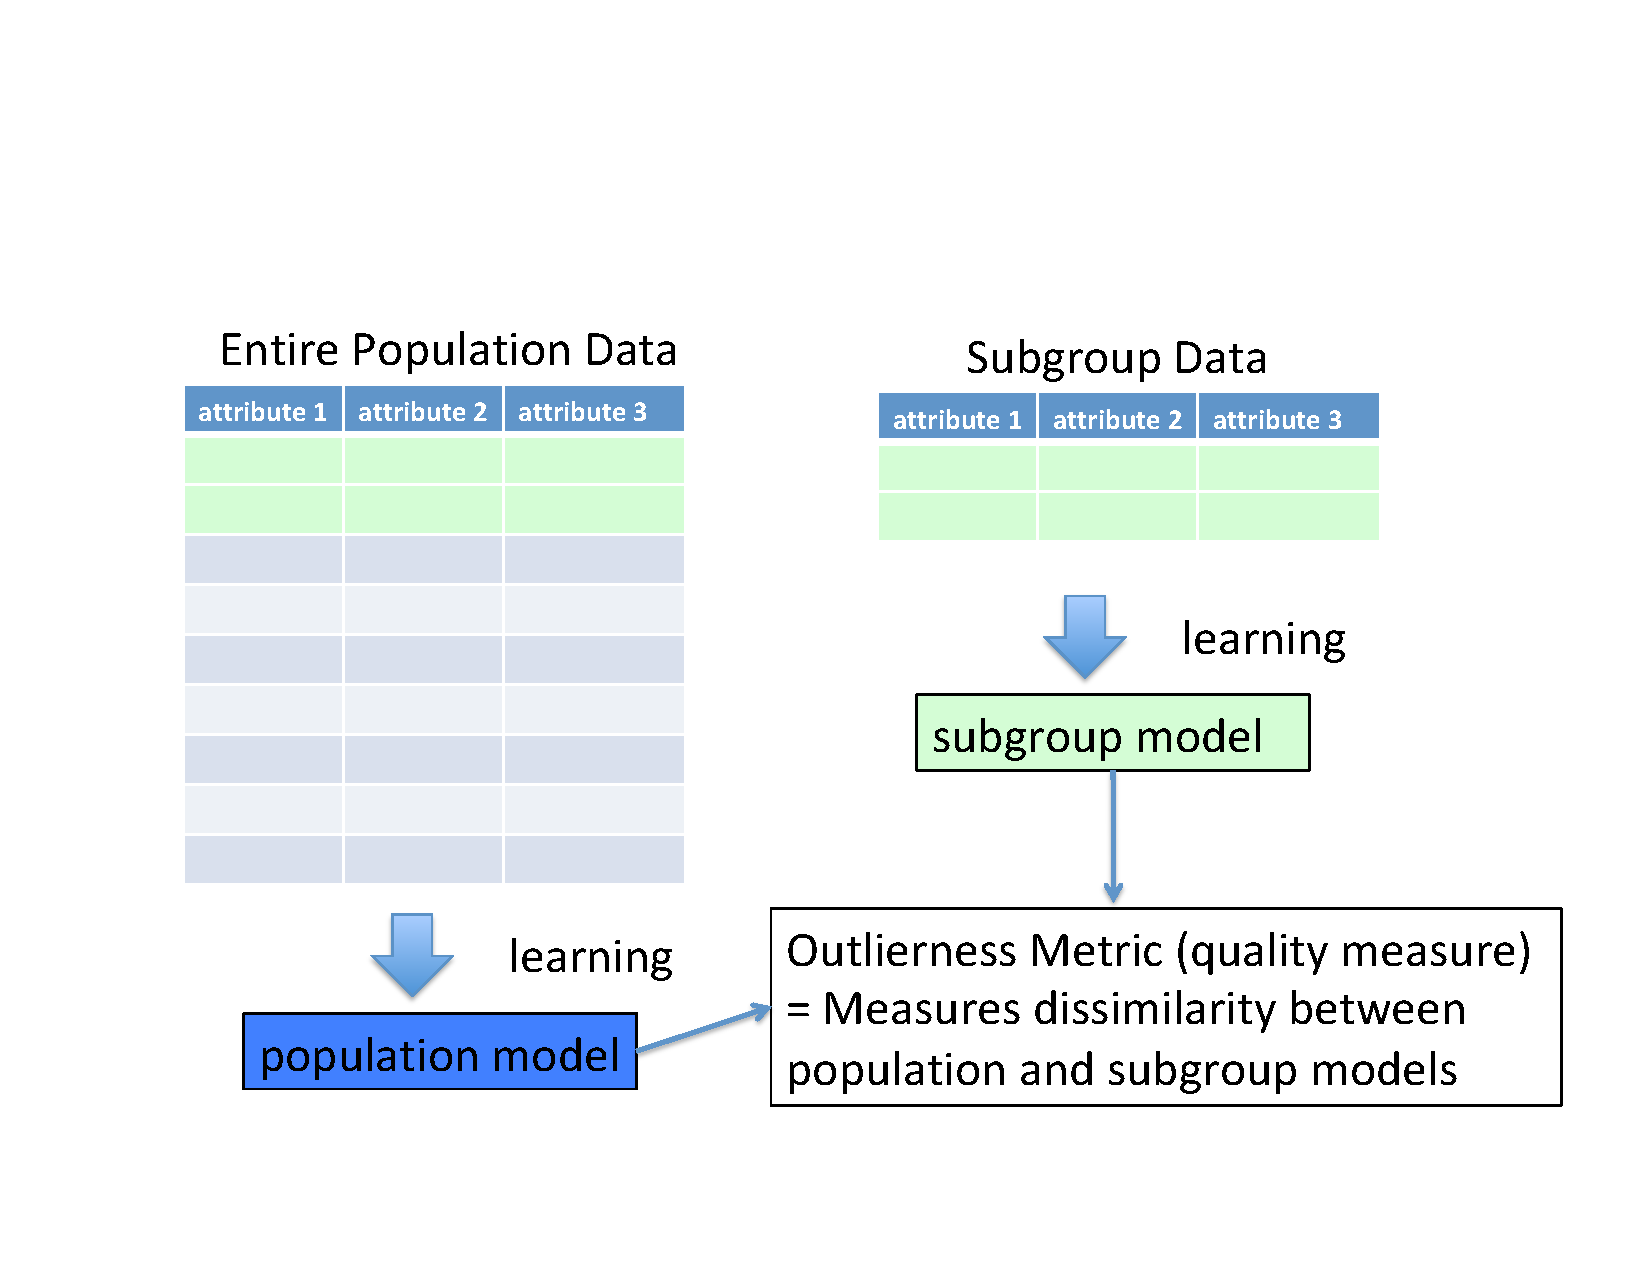
\includegraphics[width=0.7\textwidth]
{emm.pdf}
\caption{A general schema for exceptional model mining  for propositional i.i.d. data
\label{fig:emm}}
\end{figure}

{\em Model Type.} EMM is an inclusive framework in that any model type of interest can be utilized. In this paper we focus on first-order Bayesian networks (BNs)~\citep{Wang2008,Poole2003,Kimmig2014}, but our definitions apply to other log-linear models such as Markov logic networks \citep{Domingos2007}. 
A class-model Bayesian network (BN) structure is learned with data for the entire population. The nodes in the BN represent attributes for links, of multiple types, and attributes of objects, also of multiple types. To learn the BN model, we apply techniques from statistical-relational learning, a  recent field that applies and extends AI and machine learning to relational data~\citep{SRL2007,Schulte2012,Domingos2009}. For a learned BN structure, we compare two parameter vectors (see Figure~\ref{fig:flow} below): The {\em class model parameters} are estimated from the entire population data, and the {\em object model parameters} are estimated from the object data. 
% TODO: we can think of the object model as representing the role of an entity
%The BN provides dimensionality reduction, in the sense that it leverages independencies to represent the data distribution with exponentially fewer parameters than a non-factorized parametrization. 

{\em Quality Measure = Outlierness Metric.} For a given model type, quantifying the extent to which an object model deviates from the population class model is the main research question in EMM~\citep{Duivesteijn2016}. A computational method for measuring this extent is called {\em a quality measure}; when we apply EMM to relational outlier detection, we also refer to it as an {\em outlierness metric}. We propose utilizing the relational log-linear likelihood function \citep{Kimmig2014,Schulte2011} that measures how well a parametrized statistical-relational model fits an input database. The {\em likelihood ratio} is the difference in log-likelihood between the class model and the object model, when applied to the object data. Assuming maximum likelihood estimates, it is equivalent to the Kullback-Leibler divergence (KLD) between class and object models. While our evaluation indicates that KLD is a good outlierness metric, we propose improving it further by applying two transformations: (1) a mutual information decomposition, and (2) replacing log-likelihood differences by log-likelihood distances. We refer to the resulting novel score as the {\em expected log-likelihood distance} (ELD). A Taylor series analysis shows that this score  is approximated by the L1-norm (total variation distance) between the object and class data distributions.


%
%
%Given a set of parameter values and an input database, it is possible to compute a {\em class model likelihood} that quantifies how well the BN fits the object data. The class model likelihood uses BN parameter values {\em estimated from the entire class data.} This  is a relational extension of the standard log-likelihood method for i.i.d. vectorial data, which uses the likelihood of a data point as its outlierness score. %This can be adapted for object-relational data as follows.
%%The Bayes net structure represents the normal pattern of associations among links and attributes  by the well-known d-separation criterion: Two nodes are probabilistically independent if they are d-separated. 
%While the class model likelihood is a good baseline score, it can be improved by comparing it to {\em the object model likelihood}, which uses BN parameter values {\em estimated from the object data.}
%The {\em model log-likelihood ratio} (LR) is the log-ratio of the object model likelihood to the class model likelihood. This ratio quantifies how the probabilistic associations that hold in the general population deviate from the associations in the object data substructure.
%While the 
%likelihood ratio discriminates relational outliers better than the class model likelihood alone, it can be improved further by applying two transformations: (1) a mutual information decomposition, and (2) replacing log-likelihood differences by log-likelihood distances. We refer to the resulting novel score as the {\em log-likelihood distance}.
%
%This paper considers outlier detection for object-oriented data. Object-orientation is one of the main data models for representing structured data~\citep{Ramakrishnan2003,Koller1997}. It is a natural data model for the widely used XML format, where nodes in the XML document tree are viewed as objects.\footnote{\url{http://www.w3.org/DOM/}} 
%%
%%The object-oriented data model was inspired by object-oriented programming. 
%%There are different formulations of the object-oriented data model
%%; the concepts in this paper apply to data objects in general. 
%The main 
%characteristics of data objects that we utilize in this paper are the following. (1) {\em Object Identity.} Each object has a unique identifier that is the same across contexts. For example, a player has a name that identifies him in different matches. (2) {\em Class Membership.} An object is an instance of a class, which is a collection of similar objects. In particular, objects in the same class share a set of attributes. For example, van Persie is a player object that belongs to the class striker, which is a subclass of the  class player. (3) {\em Component Relationships.} Atomic objects have attributes but no components. Complex objects contain other objects as components or parts. For example, a match involves two teams, and each team comprises a set of players for that match. 
%
%%Standard outlier or anomaly detection methods are defined for a data model of atomic objects from the same class without subobjects. 
%%``flat'' feature vectors, which are atomic objects with no subobjects. 
%The class and component hierarchies represent information about objects that an outlier detection method should take into account. We achieve this in two steps. Step 1: the component hierarchy is used to compute an {\em object profile}. The object profile is a data structure that specifies the object's attributes and the attributes of related objects. Two objects are related if there is a chain of components connecting them. For example, for each soccer player, there is a player distribution over: the player's attributes, the player's team's results in matches, and the actions of the player in matches.
%%For example, for each soccer team, there is a team distribution over: the team's attributes, the team's results in matches, and the actions of the team's players in matches. 
%Step 2: Given a set of object profiles, compute an outlierness score that measures how the object's profile differs from the profiles of other objects in its class. We develop a probabilistic approach where:
%
%\begin{quote}
%	Object outlierness score = Score between object distribution and class distribution
%\end{quote}
%
%For each object, the object distribution is a joint distribution over the object's attributes and the attributes of related objects. The object distribution can be computed from counts in the object profile. The class distribution is the distribution of a randomly chosen object in the class. 
%
%
%%
%This approach allows us to apply ideas from the well-researched topic of probability divergences to the problem of object outlier detection. A baseline divergence concept is the standard Kullback-Leibler divergence (KLD). KLD computes the expected log-{\em difference} between two joint distributions. Our argument in this paper is that for outlier detection, we ought to use instead the expected log-{\em distance} between two joint distributions. The reason is that averaging distribution differences loses information when two distribution differences point in opposite directions, and cancel each other out. We refer to our novel divergence as the expected log-distance divergence (ELD).
%%\vspace{-5mm}
\paragraph{Evaluation.} Our code and data sets are available on-line at \citep{url}. We evaluate relational EMM outlierness metrics in three ways.

{\em Detection Accuracy.} Our performance evaluation follows the design of previous outlier detection studies~\citep{Gao2010,aggarwal2013},
%~\citep{Cansado2008, Muller2012},
%\footnote{review} 
where the methods are scored against a test set of known outliers.  
%and case studies assess their output on specific cases. 
%
We use three synthetic and four real-world data sets, from the UK Premier Soccer League, the Internet Movie Database (IMDb), the National Hockey League, and Mutagenesis. On the synthetic data we have known ground truth. For the real-world data sets, we use a one-class design, where one object class is designated as normal and objects from outside the class are the outliers. For example, we compare goalies as outliers against the class of strikers as normal objects. 
%Given ground truth, an outlier detection method can be scored in terms of true positives and negatives, summarized using AUC~\citep{Muller2012}.\footnote{review} 
%Comparisons outlierness scores include the class model likelihood, our novel log-likelihood distance, and likelihood-based scores intermediate to these two. 
%Previous outlier analysis for similar structured data  \citep{Breunig2000} used a preprocessing step where the structured data are converted to vectorial data that represent atomic objects. This conversion is usually done by aggregation, which tends to lose information.
%, for instance using counts as attributes in an attribute vector. After aggregation, we evaluate 
%After aggregation, standard outlier detection methods for independent data points can be applied; we use three as baseline methods for our evaluation ($\outrank$, $\lof$, and $\knn$).
Compared to six baseline methods, the EMM-based scores (likelihood ratio and expected log-likelihood distance) achieve the top detection accuracy on all three synthetic data sets, and on 4 out of 5 real-world data sets.

{\em Case Studies.} We also offer case studies where we assess whether individuals that our score ranks as highly unusual in their class are  indeed unusual. 
%This assessment looks at the object profile data of these individuals. 
The case studies illustrate that the EMM scores are {\em easy to interpret}, because the Bayesian network provides a local decomposition of log-likelihood differences. Interpretability is very important for users of an outlier detection method as there is often no ground truth to 
evaluate outliers.% suggested by the method.

{\em Correlation with Success.} We compare the likelihood-based outlierness metrics to independent success metrics for a given domain. Success rankings are one of the most interesting features to users. Our reasoning is that high success is an independent metric that indicates an unusual individual. So a correlation between an outlierness metric and success is an independent validation of the meric, and also shows that it points to meaningful and interesting outliers.

 %With regards to the cost of computing the divergence outlierness score, we show that a Bayesian network representation of the object distributions can speed up the computation by orders of magnitude.

%One of our baseline methods is a variant of the distribution divergence approach that we introduce in this paper, where Kullback-Leibler convergence is the used as the outlierness score. 
%
%we rank both normal and outlier individuals against the distribution of the normal class only. For example, we 
%compare the attribute distributions of both goalies and strikers against the class distribution of strikers. 
%
%We compare the detection accuracy of our novel mutual information divergence with the Kullback-Leibler convergence.
%basing a distribution divergence on the expected distance to basing it on the expected difference. 
%As regards to previous methods, to our knowledge ours is the first outlier detection method tailored for object-oriented data. Previous outlier analysis for structured data similar to ours (e.g., sports data) \citep{Breunig2000} used a preprocessing step where the structured data are converted to a matrix of attribute vectors that represent atomic objects. 
%  outlier detection methods for the atomic objects data model---based  on a single data matrix---have been applied to data sets similar to those that we examine  
% previously analyzed with 
%Standard outlier detection methods require as input a data matrix, that represents attributes of atomic objects from the same class. It is therefore not possible to provide structured data as input directly to such methods. In previous outlier detection work, data matrix methods were applied by 
%Converting object-oriented data to a data matrix can be done by aggregation.
%, for instance using counts as attributes in an attribute vector. After aggregation, we evaluate 
%After aggregation, standard outlier detection methods for independent data points can be applied; we use three as baseline methods for our evaluation ($\outrank$, $\lof$, and $\knn$).
% three aggregation approaches  using a subspace outlier ranking method, $\outrank$, a density-based outlier detection method, the Local Outlier Factor ($\lof$), and a distance based outlier detection method, $\knn$.  On all data sets, the log-distance divergence achieves the best detection accuracy.
%We also offer case studies where we discuss why highly ranked individuals are indeed unusual in their class. The case studies illustrate that our divergence outlierness score is easy to interpret, because it is based on a sum decomposition of the joint distributions. Interpretability is very important for users of an outlier detection method as there is often no ground truth to 
%evaluate outliers indicated by the method. 
%\vspace{-5mm}
\paragraph{Contributions} Our main contributions may be 
summarized as follows.

\begin{enumerate} 
	\item We develop the first application of the EMM framework to outlier detection for structured relational data based on a probabilistic model. 
	\item We define a new model-based outlierness score, derived from a novel model likelihood comparison, the expected log-likelihood distance.  % \footnote{Commented paper organization}
\end{enumerate}
% \vspace{-0.5cm} 
				
%				\paragraph{Previous Conference Publication.} A preliminary version of this paper appeared in the Proceedings of the IEEE SSCI series \citep{Riahi2015} (Best Student Paper). The new material in this submission comprises the following:
%				
%				\begin{enumerate} 
%				\item We expanded and clarified the relationship to previous work in EMM.
%					\item We added new experiments on the real-world data sets.
%					\item We performed a comparison between our proposed metric and a well-known relational-based distance learning method ($\textit{RIBL}$).
%					\item We introduced an application of the proposed metrics in detecting outstanding individuals and ranking them.
%					\item We applied Taylor series analysis to understand analytically the relationship between the log-likelihood ratio and the log-likelihood distance (the former is approximated by $\chi^{2}$, the latter by L1 norm). 
%				  % \footnote{Commented paper organization}
%				\end{enumerate}

\paragraph{Paper Organization} We review related work on outlier detection for structured data, then background about Bayesian networks for relational data. Then we introduce likelihood-ratio based outlierness scores for relational EMM, including our novel log-likelihood distance. 
%After presenting the details of our approach, we review related work. 
Empirical evaluation compares EMM and aggregation-based approaches to relational outlier detection, with respect to three synthetic and four real-world data sets.

				\section{Related Work}
				Outlier detection is a densely researched field; for a survey please see~\citep{aggarwal2013,Akoglu2015}.
				Figure~\ref{fig:novelty} provides a tree picture of where our method is situated with respect to other outlier detection methods and other data models. 
				%For an outlier detection survey please see~\citet{aggarwal2013}.
				%\citep{Hodge2004,aggarwal2013}. 
				Our method falls in the category of {\em unsupervised} statistical model-based approaches. To our knowledge, ours is the first model-based method tailored for object-relational data. Like EMM and other model-based approaches, it detects {\em global outliers.} \citet{aggarwal2013} defines a global outlier to be a data point that notably deviates from the rest of the population. We review relevant approaches from two different data models, the most common atomic object model---where data is represented by vectors---and structured data models. A conference presentation of part of our work is available \citep{Riahi2015}. \\
				
				% using the XML, SQL, and OLAP formats.
				%\vspace{-5mm}
				\textit{a) Attribute Vector Data Model:}
				%\footnote{\textbf{Sarah}: can you fix the silly d) for paragraph numbering?}By far most work on outlier detection considers atomic objects with flat feature vectors.
				By far most work on outlier detection considers atomic objects with flat feature vectors.
				%, or nonhierarchical structures like time series. 
				This leads to an impedance mismatch: 
				The required input format for these outlier detection methods is a single data matrix, not a structured data set. For example, one cannot provide a relational database as input. This mismatch is not simply a question of choosing a file format, but instead reflects a different underlying data model: complex objects with both attributes and component objects vs. atomic objects with attributes only. 
				%
				It is possible to ``flatten'' structured data by converting it to unstructured feature vectors, for instance by using aggregate functions. 
				%Flattening incurs some loss of information but allows us to apply the many feature vector methods.
				%\citep{Elke2013}. 
				We evaluated the aggregation approach in this paper by applying three standard methods for outlier detection.
				%for three major approaches to outlier detection: distance-based, density-based, and subspace clustering. 
				%
				%Subspace clustering methods (e.g., \citep{Muller2012,Kriegel2009}) are similar to our work in the sense that they aim to decompose a complex data space. They find complex deviations that are noticeable only in a data subspace. A common approach is to discover datapoints that show unexpected deviations in similar subspaces. Our approach instead develops a joint measure of how dissimilar the target object profile distribution is to the class distribution over the entire data space. Given that object and class distributions are represented by an object-oriented Bayesian network \citep{Koller1997}, the network structure defines subspaces. The joint divergence measure {\em mathematically decomposes} into subspace measures that quantify how dissimilar the target object profile distribution is in the subspaces defined by the network, compared to the class distribution in the same subspace.
				
				Work on atomic contextual  outliers \citep{Tang2013} is like ours in that it considers the distinctness of a target individual from a reference class. A reference class is not specified for each object,
				%as a property of the object, 
				but is constructed as part of outlier detection. 
				Our work could be combined with a class discovery approach by providing a score of how informative the inferred classes are. 
				\begin{figure}
					\centering
					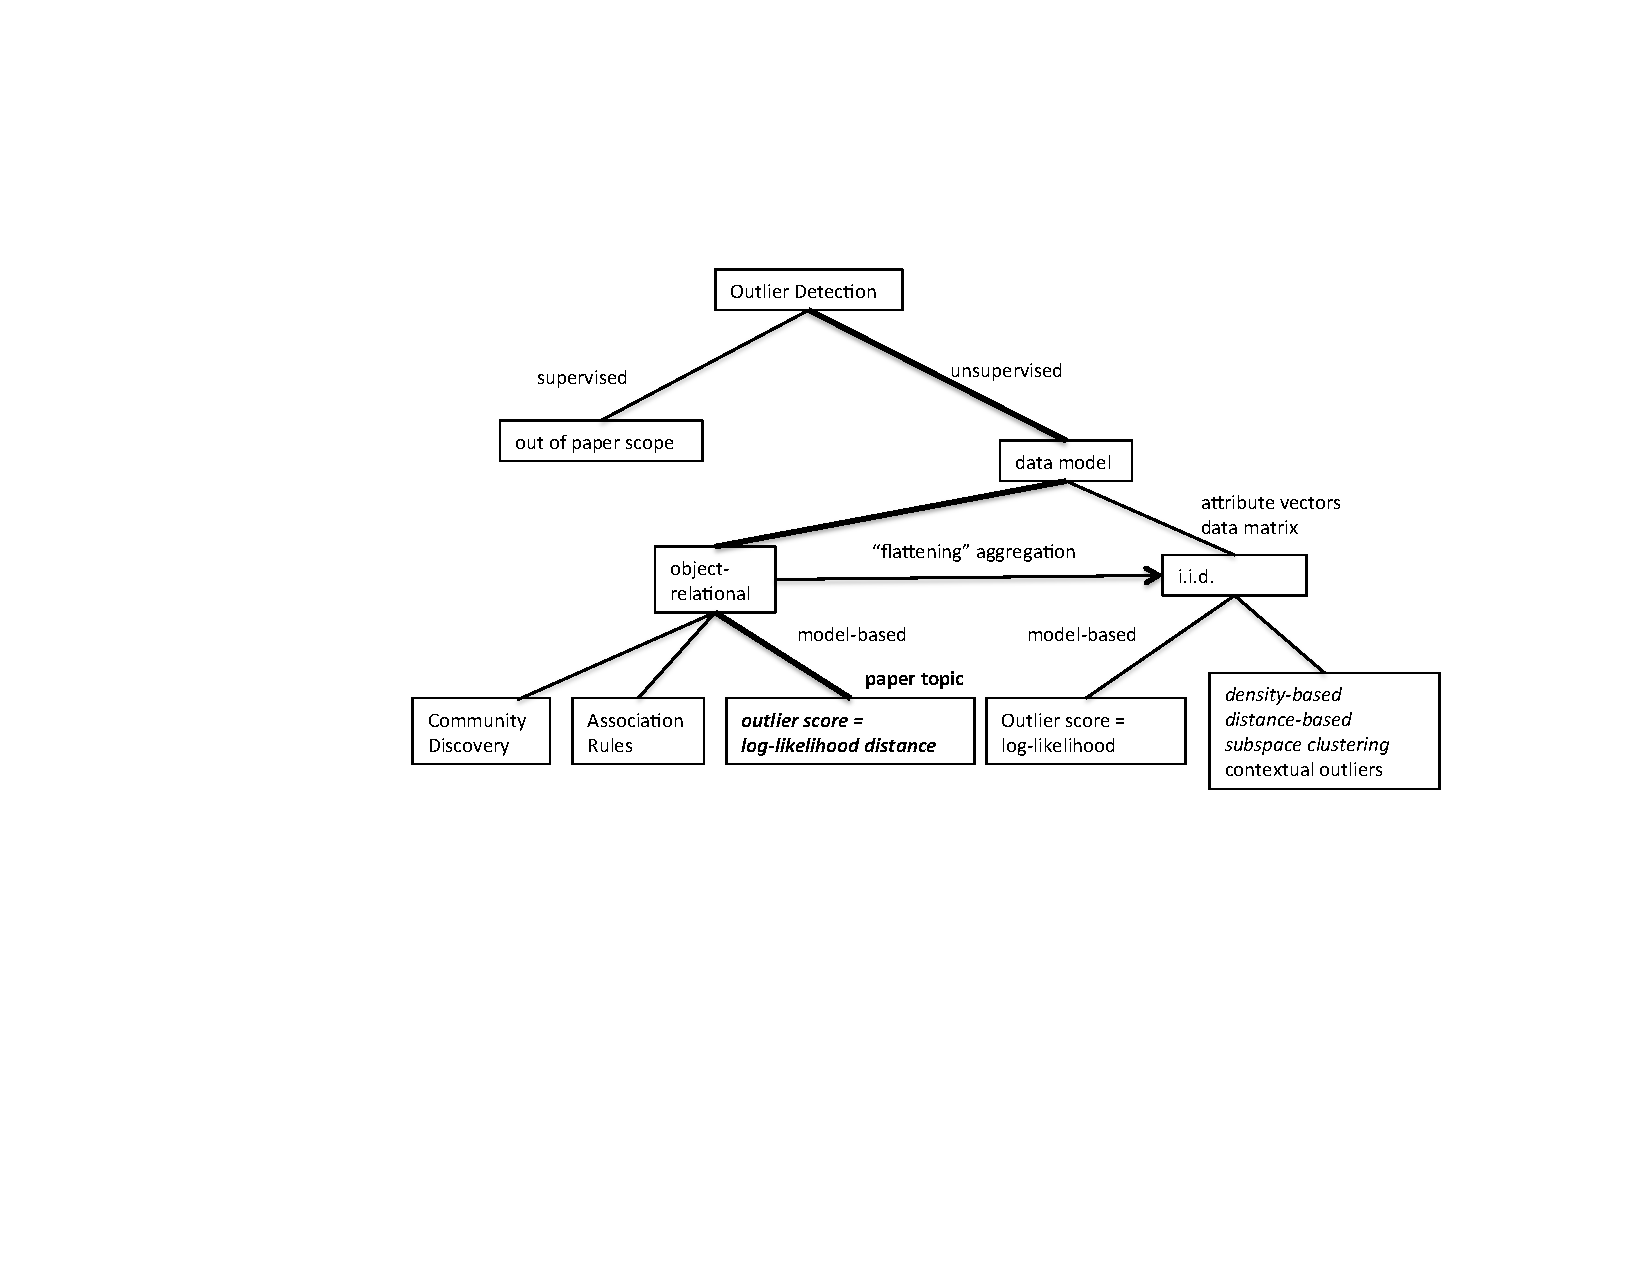
\includegraphics[width=1\textwidth] {NoveltyDiagram.pdf}
					\caption{A tree structure for related work on outlier detection for structured data. A path specifies an outlier detection problem, the leaves list major approaches to the problem. Approaches in italics appear in experiments.
						\label{fig:novelty}}
				\end{figure}
				%\vspace{-5mm}
				
				\textit{b) Structured Data Models:} We discuss related techniques in three types of structured data models: SQL (relational), XML (hierarchical), and OLAP (multi-dimensional). 
				
				For relational data, many outlier detection approaches aim to discover rules that represent the presence of anomalous associations for an individual or the absence of normal associations \citep{Maervoet2012,Gao2010}.    In these approaches what we call the object data is usually referred to as an interpretation, so the problem is to score outlier interpretations~\citep{Maervoet2012}. The survey by \citep{Novak2009} unifies within a general rule search framework three important related tasks: i) exception mining, which looks for associations that characterize unusual cases, ii) subgroup mining, which looks for associations  characterizing important subgroups, and iii) contrast space mining, which looks for differences between classes. Another rule-based approach uses Inductive Logic Programming techniques \citep{Angiulli2007}.
				%,Angiulli2009}.
				While local rules are informative, they are not based on a global statistical model and do not provide a single outlierness score for each individual. As we show in our case studies (Section~\ref{sec:CaseStudy}), the conditional probability parameters in a Bayesian network can be used to extract rules  from the BN model (of the form $\it{parent\_values} \rightarrow \it{child\_value}$).
				The distance-based algorithms designed for outlier detection can be applied to the relational case.  Horvath {\em et al.} introduced a similarity measure for the first-order instance-based learner RIBL that uses the edit distance to compute the distance between lists and terms~\citep{Horvath2001}. This distance has been used for the clustering task in~\citep{Kirsten2001}. To the best of our knowledge, distance-based relational learning has not been used for outlier detection. One-class classification can be viewed as a special case of outlier detection.  Khot {\em et al.} introduced a non-parametric relational one-class classification based on first-order trees. They proposed a tree-based distance metric to discover new relational features and to differentiate relational examples~\citep{Khot2014}. Khot {\em et al.} emphasize that their method is not appropriate for outlier detection because outlier detection makes different assumptions about the data than they do (e.g. outliers are isolated and far from other points).  
				
				 Propositionalization summarizes the multi-relational data into a single data table and can be used for outlier detection and classification tasks~\citep{Kramer2000,Lavrac13,kuzelka2008,Riahi2016,AndersonP08}. 
				
				A latent variable approach in information networks ranks potential outliers in reference to the latent communities inferred by network analysis \citep{Gao2010}. Our model also aggregates information from entities and links of different types, but does not assume that different communities have been identified. 
				
				
				Koh {\em et al.}~\citep{Koh2008} propose a method for hierarchical structures represented in XML document trees. Their aim is to identify feature outliers, not class outliers as in our work. Also, they use aggregate functions to convert the object hierarchy into feature vectors. Their outlierness score is based on local correlations, and they do not construct a model.
				
				
				The multi-dimensional data model defines numeric measures for a set of dimensions. 
				%A seminal approach to exploring a multi-dimensional datacube was presented by Sarawagi {\em et al.}~\citep{Sarawagi1998}. 
				%The object and the multi-dimensional data models are similar in the respect that both objects and dimensions are ordered in a hierarchy. However, 
				The differences in the two data models mean that multi-dimensional outlier detection models~\citep{Sarawagi1998} do not carry over to object-relational outlier detection. (1) The object data model allows but does not require any numeric measures. In our data sets, all features are discrete. Nor do we assume that it is possible to aggregate numeric measures to summarize lower-level data at higher levels.  
				(2) In scoring a potential outlier object, our method considers other objects {\em both} below and above the target object in the component hierarchy. OLAP exploration methods consider only cells below or at the same level as the target cell. For example, in scoring a player, our method would consider features of the player's team.  
				Also, the $\mid$ outlierness score of an object is not determined by the outlierness scores of its components, in contrast to approaches derived from Sarawagi {\em et al.}~\citep{Sarawagi1998}. They use values such as the most unusual cell that is below a target cell.
				(3) Our approach models a joint distribution over features, exploiting correlations among features. Most of the OLAP-based methods consider only a single numeric measure at a time, not a joint model.  




\section{Background: Bayesian Networks for Relational Data}
We adopt  
the first-order Bayesian network (PBN) formalism \citep{Poole2003} that combines Bayesian networks with logical syntax for expressing relational concepts. 


\subsection{Relational Data}




%We apply the learn-and-join algorithm (LAJ), which is the state-of-the-art Bayes net learning method for relational data. The LAJ algorithm takes as input a relational database and outputs a Bayes net using the functor notation due to Poole \citep{Poole2003}. We briefly review this notation.

%\paragraph{Functor Terms} 
We adopt a term-based notation for combining logical and statistical concepts~\citep{Poole2003,Kimmig2014,Wang2008}. {Table~\ref{table:notation} summarizes our notation.
A functor is a function or predicate symbol. Each functor has a set of values (constants) called the \textbf{domain} of the functor. The range of a \textbf{predicate} is $\{\true,\false\}$. Predicates are usually written with uppercase Roman letters, other terms with lowercase letters.
A predicate of arity at least two is a \textbf{relationship} functor. Relationship functors specify which objects are linked. Other functors represent \textbf{features} or \textbf{attributes} of an object or a tuple of objects (i.e., of a relationship).
A \textbf{population} is a set of objects. 
A \textbf{term} is of the form $f(\term_{1},\ldots,\term_{k})$ where $\functor$ is a functor %(either a function symbol or a predicate symbol) 
and each $\term_{i}$ is a first-order variable or a constant denoting an object. A term is \textbf{ground} if it contains no first-order variables; otherwise it is a first-order term. In the context of a statistical model, we refer to first-order terms as \textbf{first-order random variables} (FORVs) \citep{Wang2008,Schulte2017a}. 
%A term whose range are the truth values $\{\true,\false\}$ is a \textbf{predicate}. 
%Predicates are usually written with uppercase Roman letters, other term with lowercase letters.
%The grounding concept represents moving from the population-level  to the object level. 
A \textbf{grounding} replaces each first-order variable in a term by a constant; the result is a ground term. A grounding may be applied simultaneously to a set of terms.  A relational database $\D$ specifies the values of all ground terms. %, which can be listed in data tables. 
%In machine learning terminology, the data tables are contingency tables that represent sufficient statistics or event counts.

Consider a joint assignment 
$P(\Features = \set{\nodevalue})$ of values to a set of FORVs $\Features$. The {\em grounding space} of the FORVs is the set of all possible grounding substitutions, each applied to all FORVs in $\Features$. The {\em count} of groundings that satisfy the assignment with respect to a database $\D$ is denoted by $\grounds_{\D}(\Features = \set{\nodevalue})$. The \textbf{database frequency} $P_{\D}(\Features = \set{\nodevalue})$ is the grounding count divided by the number of all possible groundings~\citep{Halpern90,Schulte2014}. %Table~\ref{table:notation} contains a complete set of notations used in this paper.
%, that is, the size of the grounding space.
 	 	      \begin{table} 
 	 	     
 	 	      	\centering
 	 	      	\resizebox{1\textwidth}{!}{
 	 	      		\begin{tabular}{ll}
 	 	      			\hline
 	 	      			Symbol&Definition\\\hline
 	 	      			$\a,\b,\a_{1},\b_{1},\ldots$ & Constant \\\hline
 	 	      			$\A,\B,\it{T},\it{M},\ldots$ & First-order variable
 	 	      			\\\hline $\functor,g,\ldots,$ & Functor, function symbol
 	 	      			\\\hline
 	 	      			$\functor(\A,\ldots,\A_{k})$& First-order term\\\hline
 	 	      			$\functor(\A=\a_{1},\ldots,\A_{k}=\a_{k})$ & Ground term \\\hline
 	 	      			$\D$& Relational database\\\hline
 	 	      			$\D_{\Class}$ &Database for the entire class of objects\\\hline
 	 	      			$\D_{\object}$& Restriction of the input database to the target object\\\hline
 	 	      			$\feature(\A,...,\B)$& A first-order random variable\\\hline
 	 	      			$\Features $&A set of first-order random variable\\\hline
 	 	      			%  $\{\nodevalue_{i1},\ldots,\nodevalue_{i\states_{i}}\}$&Possible values of $\feature_{A,B,...}$\\\hline
 	 	      			$\Features = \set{\nodevalue}$& Joint assignment of values to a set of FORVs\\\hline
 	 	      			$P(\Features = \set{\nodevalue}) \equiv P(\set{\nodevalue})$ &Joint probability that each variable $\feature_{i}$ takes on value $\set{\nodevalue}_{i}$\\\hline
 	 	      			$\grounds_{\D}(\Features = \set{\nodevalue})$& Count of groundings that satisfy the assignment\\\hline
 	 	      			
 	 	      			$\A$\textbackslash$v$& Ground a first-order variable\\\hline
 	 	      			
 	 	      			$\model$&A Bayesian network structure\\\hline
 	 	      			$\model_{\Class}$ & A Bayesian network structure learned with $\D_{\Class}$ as the input database\\\hline
 	 	      			$\parameters_{\Class}$ & Parameters learned for $\model_{\Class}$ using $\D_{\class}$  as the input database\\\hline
 	 	      			$\parameters_{\object}$ & Parameters learned for $\model_{\Class}$ using $\D_{\object}$  as the input database\\\hline
 	 	      			$\parents_{i}$&Parent of node $i$\\\hline
 	 	      			% $\parameters_{\object}$ are parameters learned for $\model_{\Class}$ using $\D_{\class}$ resp. $\D_{\object}$ as the input database.
 	 	      			%Synthetic&40&280\\ \hline
 	 	      		\end{tabular}} 	\caption[Table of Notations]{Notation and Definition	\label{table:notation}}
 	 	      	\end{table}\\
			
			\paragraph{Example.}
\label{sec:example}
%
The Opta data set represents information about Premier League data %\citep{opta-original} 
(Sec.~\ref{sec:real}). 
%Using the functor notation, the data
%format can be represented as follows. 
The basic populations are teams, players, matches, with 
corresponding first-order variables $\team, \player, \match$. As shown in Table~\ref{table:data}, the groundings count can be visualized in terms of a groundings table ~\citep{Schulte2014}, also called a universal schema~\citep{Riedel2013}. 
%Table~\ref{table:data} specifies values for some ground terms. 
The first three column headers show first-order variables ranging over different populations. The remaining columns represent terms. Each row represents a single grounding and the values of the ground terms defined by the grounding.
%Table~\ref{table:counts} illustrates grounding counts. 
In terms of the grounding table, the grounding count of a joint assignment is the number of rows that satisfy the conditions in the joint assignment. The database frequency is the grounding count divided by the total number of rows in the groundings table. Table~\ref{table:counts} shows an example of computing frequencies. Counts are based on the 2011-2012 Premier League Season. We count only groundings $(\it{team},\it{match})$ such that $\it{team}$ plays in $\it{match}$. Each team, including Wigan Athletic, appears in 38 matches. The total number of team-match pairs is $38 \times 20 = 760$.

%Examples of terms include the following. 

%\begin{itemize}
%\item $\it{Appears\_Player}(\P,\M)$ indicates whether a player appeared in a match.
%\item $\it{Appears\_Team}(\T,\M)$ indicates whether a team played in a match.
%\item $\it{Team}(\P)$ returns the team of a player.
%\item $\it{Result}(\T,\M)$ denotes the result of a team in a match (win or lose).
%\item $\it{ShotEff}(\T,\M)$ denotes the shot efficiency of a team in a match (number of successful shots on target, per total number of shots).
%\item $\it{TimePlayed}(\P,\M)$ denotes the total time that a player played in a match.
%\end{itemize}


%\begin{table}[htbp]
%\caption{Examples of terms in the soccer data set.}
%\centering
%\resizebox{1\textwidth}{!}{
%\begin{tabular}{|c|p{5cm}|}
%\hline
%Term&Meaning\\ \hline
%$\it{Appears\_Player}(\P,\M)$ & indicates whether a player appeared in a match.\\ \hline
%$\it{Appears\_Team}(\T,\M)$&indicates whether a team played in a match.\\ \hline
%$\it{Team}(\P)$& returns the team of a player.\\ \hline
%$\it{Result}(\T,\M)$ &denotes the result of a team in a match (win or lose).\\ \hline
%$\it{ShotEff}(\T,\M)$ &denotes the shot efficiency of a team in a match (number of successful shots on target, per total number of shots).\\ \hline
%$\it{TimePlayed}(\P,\M)$& denotes the total time that a player played in a match.\\ \hline
%\end{tabular}}
%\label{table:terms}
%\end{table}

\begin{table}[htbp]

	\centering
	\resizebox{1\textwidth}{!}{
		\begin{tabular}{cclccc}
			\hline
			\multicolumn{1}{l}{MatchId \match} &
			TeamId \team & PlayerId \player
			& \multicolumn{1}{l}{TimePlayed(\player,\match)} & 
			\multicolumn{1}{l}{ShotEff(\team,\match)}&result(\team,\match) \\ \hline
			117 & WA & McCarthy  & 90 & 0.53&win\\ \hline
			148 & WA & McCarthy  & 85 & 0.57&loss\\ \hline
			15 & MC & Silva  & 90 & 0.59&win\\ \hline
			\ldots& \ldots &\ldots&\ldots&\ldots&\ldots\\
		\end{tabular}}	\caption{Sample Population Data Table (Soccer). \label{table:data}}

		\resizebox{1\textwidth}{!}{
			\begin{tabular}{cclccc}
				\hline
				\multicolumn{1}{l}{MatchId \match} &
				TeamId $\team = \it{WA}$ & PlayerId \player& \multicolumn{1}{l}{TimePlayed(\player,\match)} & 
				\multicolumn{1}{l}{ShotEff(\it{WA},\match)}&result(\it{WA},\match) \\ \hline
				117 & WA & McCarthy  & 90 & 0.53&win\\ \hline
				148 & WA & McCarthy  & 85 & 0.57&loss\\ \hline
				\ldots& WA &\ldots&\ldots&\ldots&\ldots\\
			\end{tabular}}		\caption{Sample Object Data Table, for team $\team = \it{WA}$; all rows have WA in the $T$ column. \label{table:individual}}
		\end{table}
		
		
		
		
		A novel aspect of our paper is that we {\em learn model parameters for specific objects as well as for the entire population.}
		%To implement this, for each target object, we form 
		The appropriate \textbf{object data table} is formed from the population data table by restricting the relevant first-order variable to the target object. 
		For example, the object database for target Team $\it{Wigan Athletic}$, 
		forms a subtable of the data table of Table~\ref{table:data} that contains only rows where 
		TeamID = $\it{WA}$; see Table~\ref{table:individual}. In database terminology, an object database is like a view centered on the object.
		
		%\begin{table} 
		%	\captionsetup{singlelinecheck=off}
		%			\caption[.]{\label{table:counts}Example of Grounding Count and Frequency for the conjunction \begin{displaymath} \it{passEff(T,M)=hi}, shotEff(T,M)=high, Result(T,M)=1.\end{displaymath}}
		%			\centering
		%			\resizebox{1\textwidth}{!}{
		%				\begin{tabular}{|c|c|c|}
		%					\hline
		%					Database&Count or $\#_{D}(\Features = \set{\nodevalue})$&Frequency or $P_{D}(\Features = \set{\nodevalue})$\\\hline
		%					Population&76& $76/760=0.10$\\\hline
		%					Wigan Athletic&7&$7/38=0.18$\\\hline
		%		
		%					%Synthetic&40&280\\ \hline
		%				\end{tabular}}
		%			\end{table}
		\begin{table} 

			\centering
			\resizebox{1\textwidth}{!}{
				\begin{tabular}{ccc}
					\hline
					Database&Count or $\#_{D}(\Features = \set{\nodevalue})$&Frequency or $P_{D}(\Features = \set{\nodevalue})$\\\hline
					Population&76& $76/760=0.10$\\\hline
					Wigan Athletic&7&$7/38=0.18$\\\hline
					
					%Synthetic&40&280\\ \hline
				\end{tabular}}			\caption{Example of Grounding Count and Frequency in Premier League Data, for the conjunction $\it{passEff(T,M)=hi}, shotEff(T,M)=hi, Result(T,M)=win$.\label{table:counts}}
			\end{table}
			
			%\begin{table} 
			%	\captionsetup{singlelinecheck=off}
			%			\caption[.]{\label{table:counts}Example of Grounding Count and Frequency for the conjunction \begin{displaymath} \it{passEff(T,M)=hi}, shotEff(T,M)=high, Result(T,M)=1.\end{displaymath} Counts are based on the 2011-2012 Premier League Season. We count only groundings $(\it{team},\it{match})$ such that $\it{team}$ plays in $\it{match}$. Each team, including Wigan Athletic, appears in 38 matches. The total number of team-match pairs is $38 \times 20 = 760$.
			%			\label{MetricComputation}}
			%			\centering
			%			\resizebox{1\textwidth}{!}{
			%				\begin{tabular}{|c|c|c|}
			%					\hline
			%					Database&Count or $\#_{D}(\Features = \set{\nodevalue})$&Frequency or $P_{D}(\Features = \set{\nodevalue})$\\\hline
			%					Population&76& $76/760=0.10$\\\hline
			%					Wigan Athletic&7&$7/38=0.18$\\\hline
			%		
			%					%Synthetic&40&280\\ \hline
			%				\end{tabular}}
			%				
			%			\end{table}
			
			%[Example of counts, frequencies]
			% For simplicity only, suppose that the only matches and players in the season are those shown in Table~\ref{table:data}. Then the attribute value $\it{First\_goals} = 0$ occurs with frequency $1/2$ in the object distribution $P_{\it{si}}$ for Silca. In the player class distribution $P_{\it{Player}}$, the attribute value $\it{First\_goals} = 0$ occurs with frequency $4/5$. So Silva is somewhat less likely to score no goal than a randomly selected player.
			

\subsection{Bayesian Networks}

A Bayesian network (BN) structure $\model$ is a Directed Acyclic Graph (DAG)  whose nodes comprise a set of random variables \citep{Pearl1988}. Depending on context, we interchangeably refer to the nodes  and variables of a BN, collectively denoted by $\Features = \{\feature_{1},\ldots,\feature_{n}\}$. 
%These are attributes of objects, which can and typically do belong to different classes. In statistical terms, each attribute defines a random variable. 
The possible values of $\feature_{i}$ are enumerated as $\{\nodevalue_{i1},\ldots,\nodevalue_{i\states_{i}}\}$. The notation $P(\feature_{i} = \nodevalue)\equiv P(\nodevalue)$ denotes the probability of variable $\feature_{i}$ taking on value $\nodevalue$. We also use the vector notation $P(\Features = \set{\nodevalue}) \equiv P(\set{\nodevalue})$ to denote the joint probability that each variable $\feature_{i}$ takes on value $\set{\nodevalue}_{i}$. 


The conditional probability parameters of a Bayesian network specify the distribution of a child node given an assignment of values to its parent nodes. For an assignment of values to its nodes, a BN defines the joint probability as the product of the conditional probability of the child node value given its parent values, for each node in the network. This means that the log-joint probability can be {\em decomposed} as the node-wise sum

\begin{equation} \label{eq:bn}
\ln P(\Features = \set{\nodevalue};\model,\parameters) = \sum_{i=1}^{n} \ln \parameter(\set{\nodevalue}_{i}|\set{\nodevalue}_{\parents_{i}})
\end{equation}

\noindent where $\set{\nodevalue}_{i}$ is the assignment of values to node $\feature_{i}$, and $\set{\nodevalue}_{\parents_{i}}$  is the assignment of values to the parents of $\feature_{i}$, as determined by the assignment $\set{\nodevalue}$. 
%The function $\ln$ is the binary logarithm base 2. 
To avoid difficulties with $\ln(0)$, here and below we assume that joint distributions are positive everywhere. Since the parameter values $\parameters$ for a Bayesian network define a joint distribution over its nodes, they therefore entail a marginal, or unconditional, probability for a single node. We denote the \textbf{marginal probability} that node $\feature$ has value $\nodevalue$ as $P(\feature = \nodevalue;\model,\parameters) \equiv \parameter(\nodevalue)$. In the following we use the term Bayesian network model to refer to a network structure with parameters (i.e., a pair $(\model,\parameters)$); for brevity, we also use the terms ``Bayesian network'' or ``model''. 

\paragraph{Example.} Figure~\ref{fig:bn-imdb} shows an example of a Bayesian network model and associated conditional and marginal probabilities. 

\begin{figure}[t]
 		\centering
 		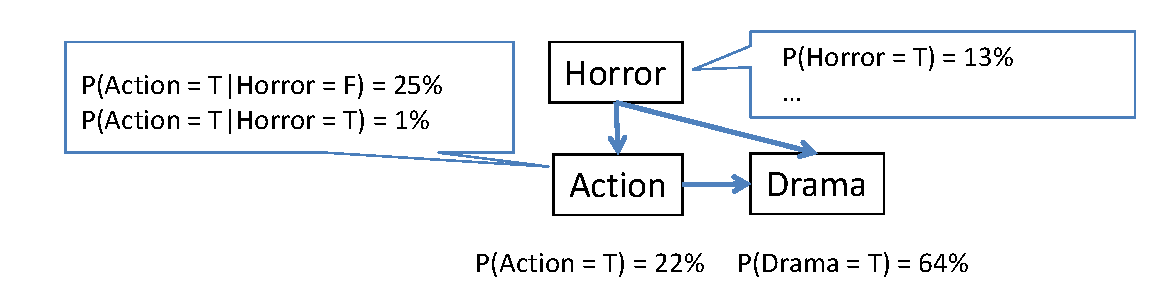
\includegraphics[width=1\textwidth] 
 		{movie-bn.pdf}
 		\caption[Example of conidtional and marginal probabilities computed from a toy Bayesian network structure. ]{Example of joint and marginal probabilities computed from a simple Bayesian network structure that was learned from the $\it{Movies}$ table in the IMDb data set described in Section~\ref{sec:real}. The parameters were estimated from the  IMDb data set. The conditional probability parameters for the $\it{Drama}$ node are not shown. The Bayesian  network shows that movie genres are largely but not completely exclusive. For instance, among horror movies, only 1\% are also classified as action movies. The marginal probabilities are the base rate frequencies of horror, action, and drama movies, which are respectively 13\%, 22\%, 64\%.
 			%We show only the Markov blanket of the Results node to simplify. 
 			\label{fig:bn-imdb}
 		}
 	\end{figure}


%

%				\begin{figure}
%				\centering
%				\resizebox{0.9\textwidth}{!}{
%				
%				\subfigure{
%				  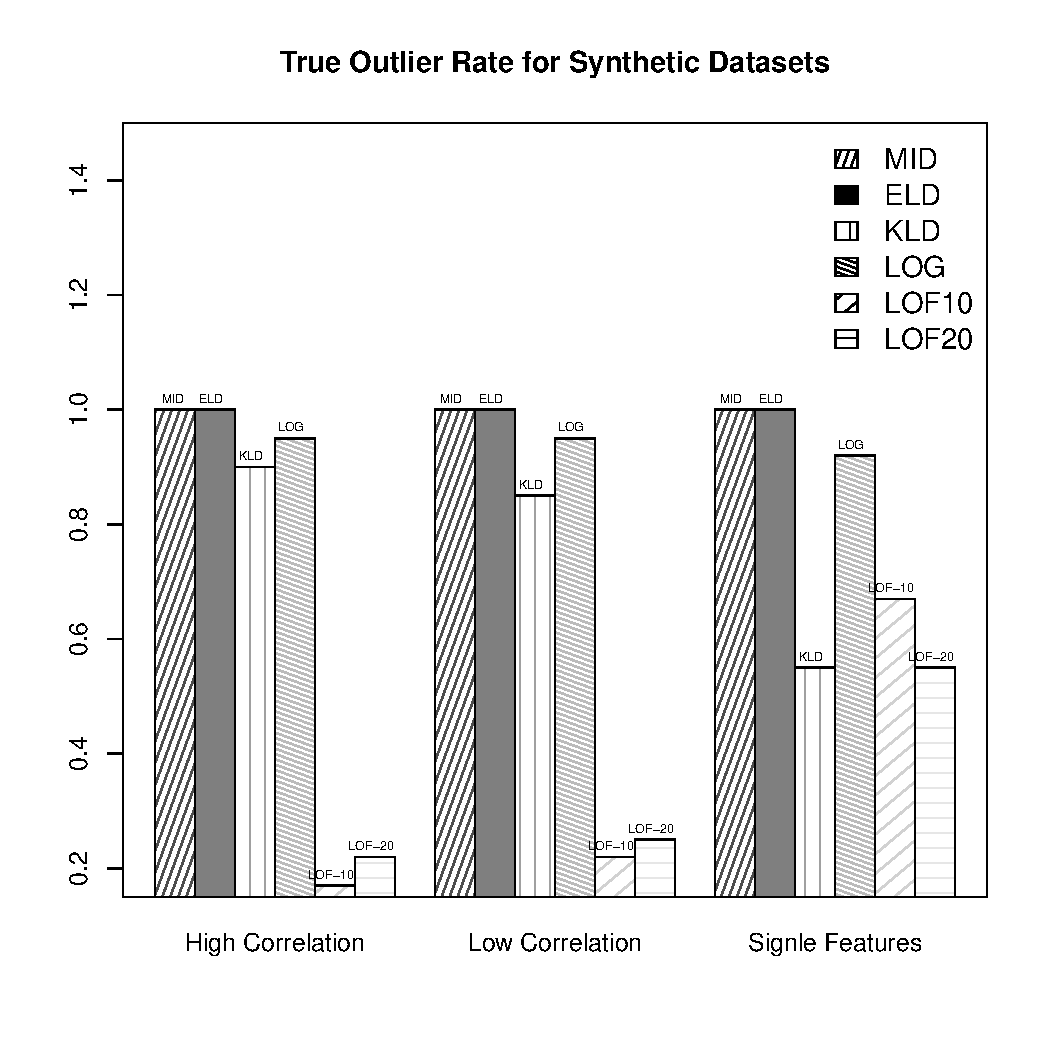
\includegraphics[height=70mm, width=70mm] {figures/TPR-Synthetic.pdf}
%				}
%				\subfigure{
%				  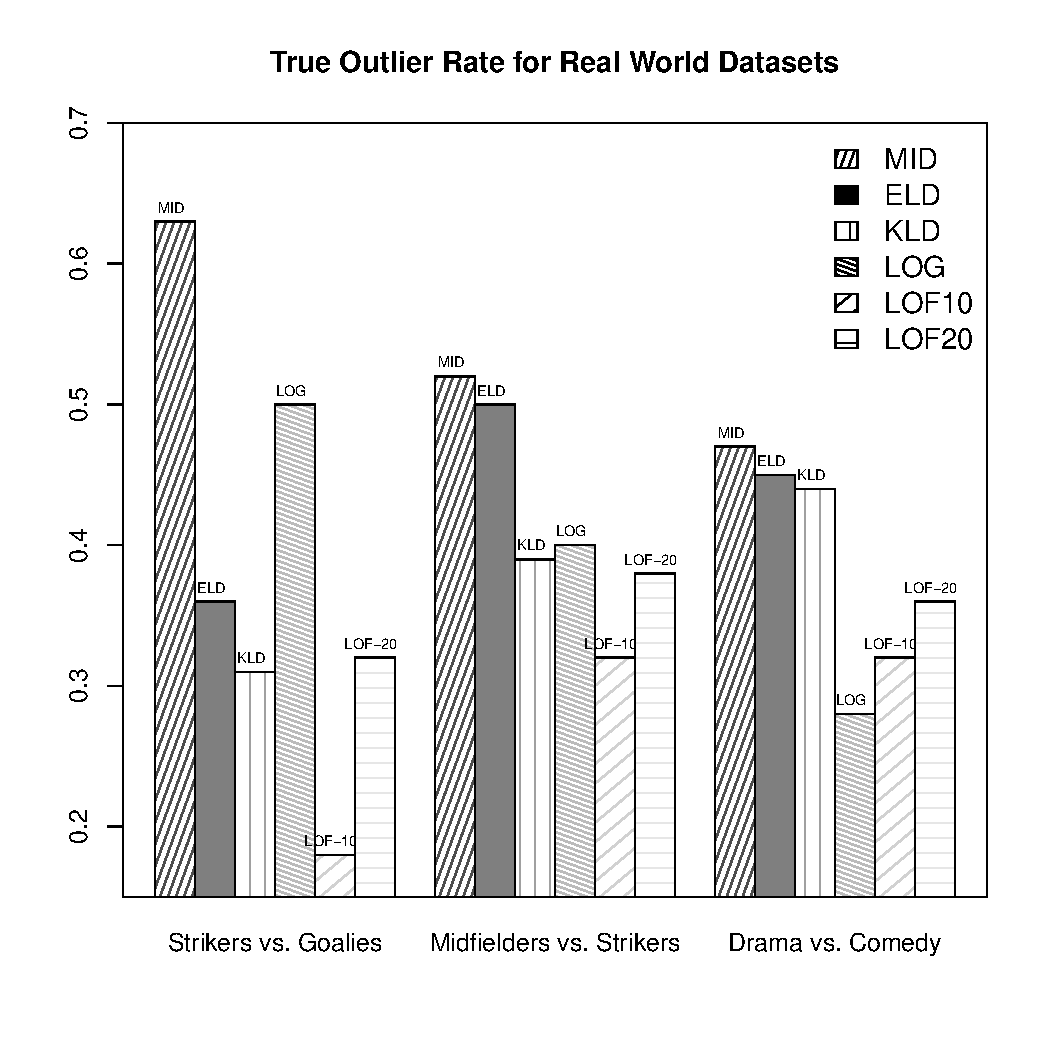
\includegraphics[height=70mm, width=70mm] {figures/TPR-All.pdf}
%				
%				 }
%				 }
%				
%				\caption{Comparison of Object Outlier Metrics}
%				\label{fig:synthetic}
%				\end{figure}
%				

%				\begin{figure}
%					\centering
%					\begin{subfigure}{0.4\textwidth}
%						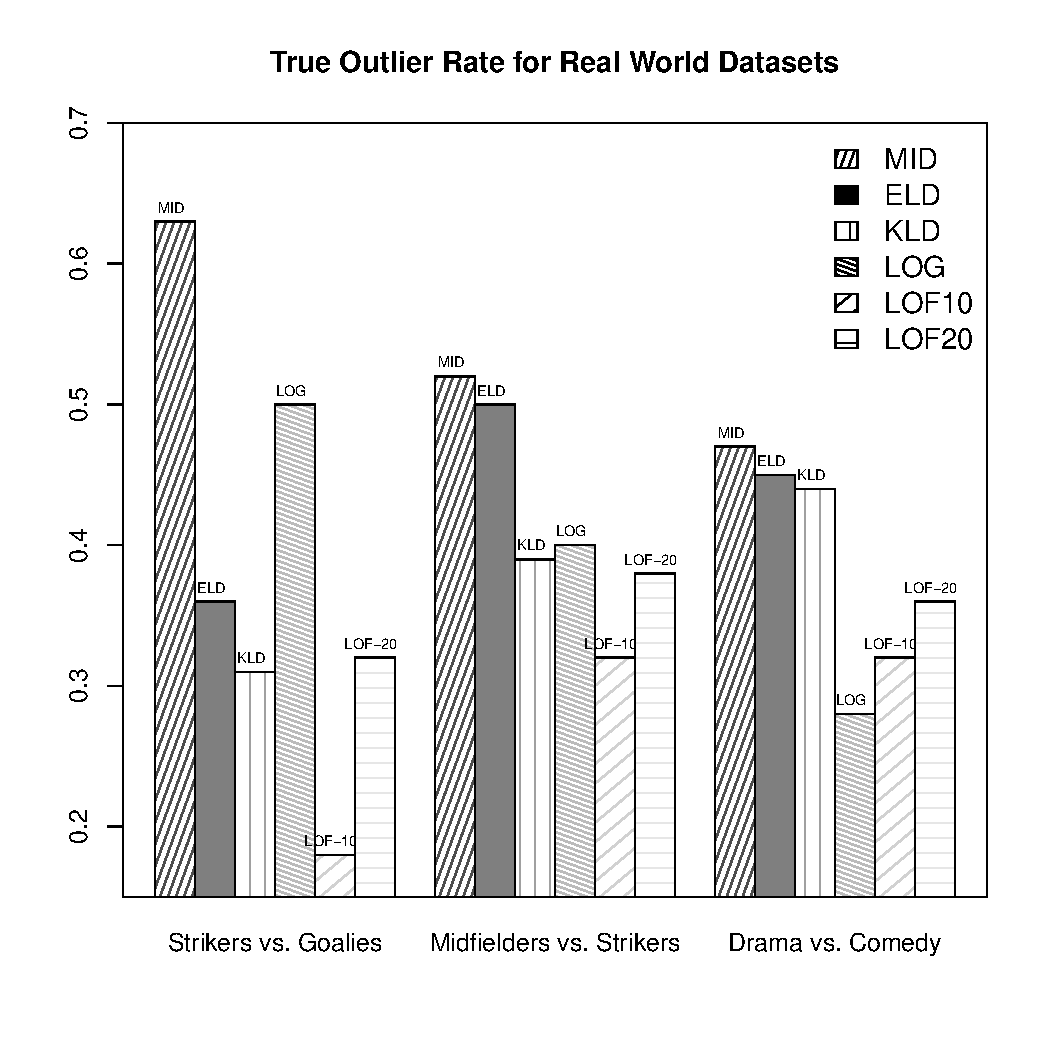
\includegraphics[width=1\linewidth]{figures/TPR-All.pdf}
%						\caption{}
%						\label{fig:Ng1} 
%					\end{subfigure}
%					
%					\begin{subfigure}{0.4\textwidth}
%						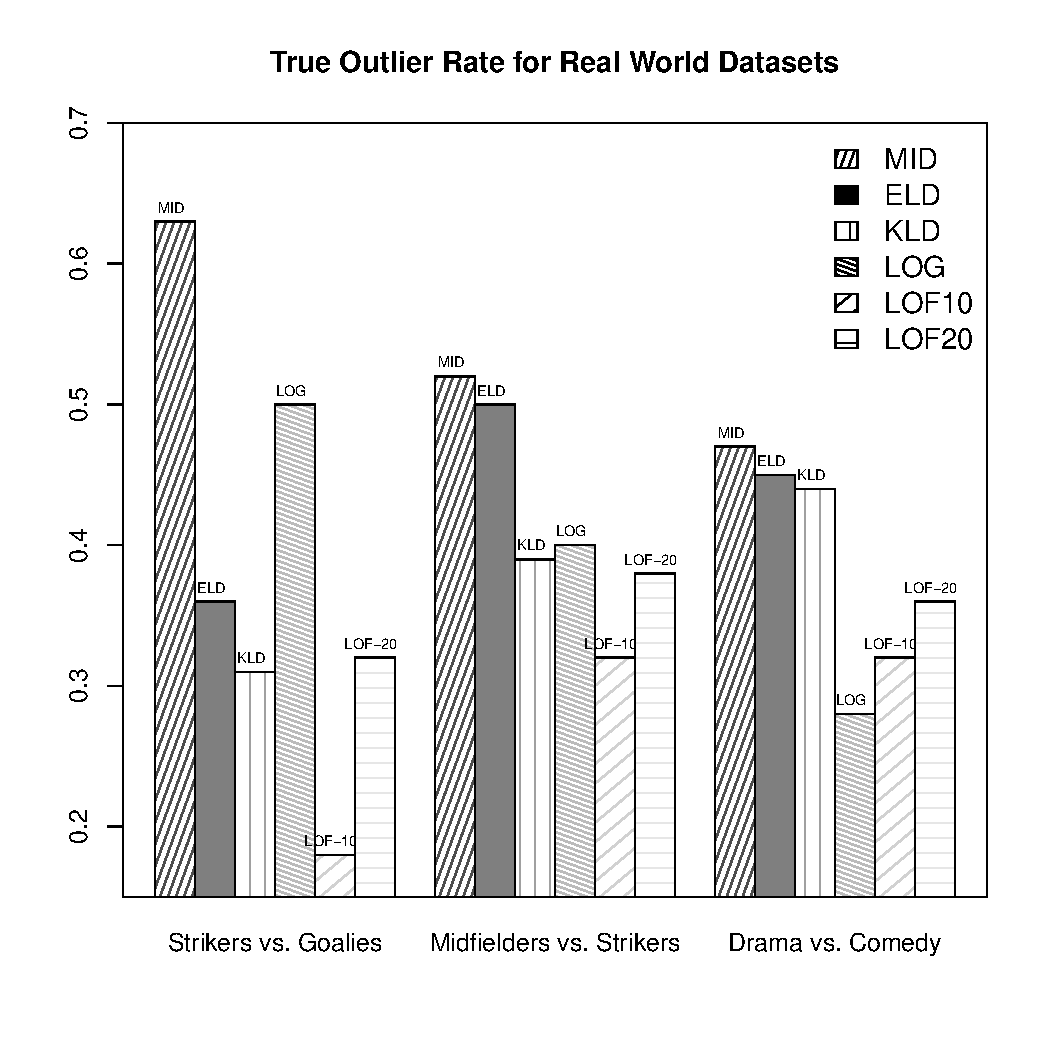
\includegraphics[width=1\linewidth]{figures/TPR-All.pdf}
%						\caption{}
%						\label{fig:Ng2}
%					\end{subfigure}
%					
%					\caption[Two numerical solutions]{(a) Numerical solutions for the small-time system 
%						with a constant-curvature body shape showing the scaled leading-order veritcal 
%						reaction force $N_0$ versus the scaled body mass $M$ for various values of $g$. 
%						Again, $I=M$ for definiteness and $A=0.7$. (b) As for (a) but over a wider range of 
%						values of $M,I$.}
%				\end{figure}

			\subsection{Target Model: Bayesian Networks for Relational Data}
			
			A \textbf{first-order Bayesian Network Structure} (FOBN) 
			%also called a first-order Bayesian network, 
			is a Bayesian network structure  whose nodes are FORVs~\citep{Poole2003,Wang2008,Schulte2017a}. 
			%For most of the paper we refer to FOBNs simply as Bayesian networks, and to FORVs simply as random variables. 
			%The learn-and-join algorithm is the state-of-the-art Bayes net learning method for relational data, based on model search in the lattice of relationship joins \citep{Schulte2012}. The LAJ algorithm takes as input a relational database and outputs a first-order Bayes net structure.
			%We review the algorithm very briefly; for further details please see \citep{Schulte2012}. 
			%The algorithm builds a Bayes net for an entire database by level-wise search through the {\em lattice of relationship chains.} This is the lattice of relationship sets that are connected by shared first-order variables.
			%%; see Figure~\ref{fig:lattice}.  
			%%We describe the fundamental ideas of the algorithm; for further details please see \citep{Schulte2012}. 
			%The user chooses a single-table Bayes net learner. The learner is applied to base population data tables. Then the learner is applied to data tables for relationship chains of size $s,s+1,\ldots$, with the constraint that the models for larger join tables inherit the absence or presence of learned edges from smaller join tables. 
			%
			The relationships and features in an object database define a set of nodes for a first-order Bayesian network. I.i.d. data represented in a single table
can be viewed as a {\em special limiting case of multi-relational data with no relationships}\citep{Nickel2016,Knobbe2006}. Syntactically, this means that columns in an i.i.d. data table represent unary functors, where the relevant population is assumed to be clear from the context rather than explicitly specified as a first-order variable. Figure~\ref{fig:bn-imdb2} illustrates how the usual syntax for i.i.d. Bayesian networks is a special case of the FOBN syntax.

\begin{figure}[t]
 		\centering
 		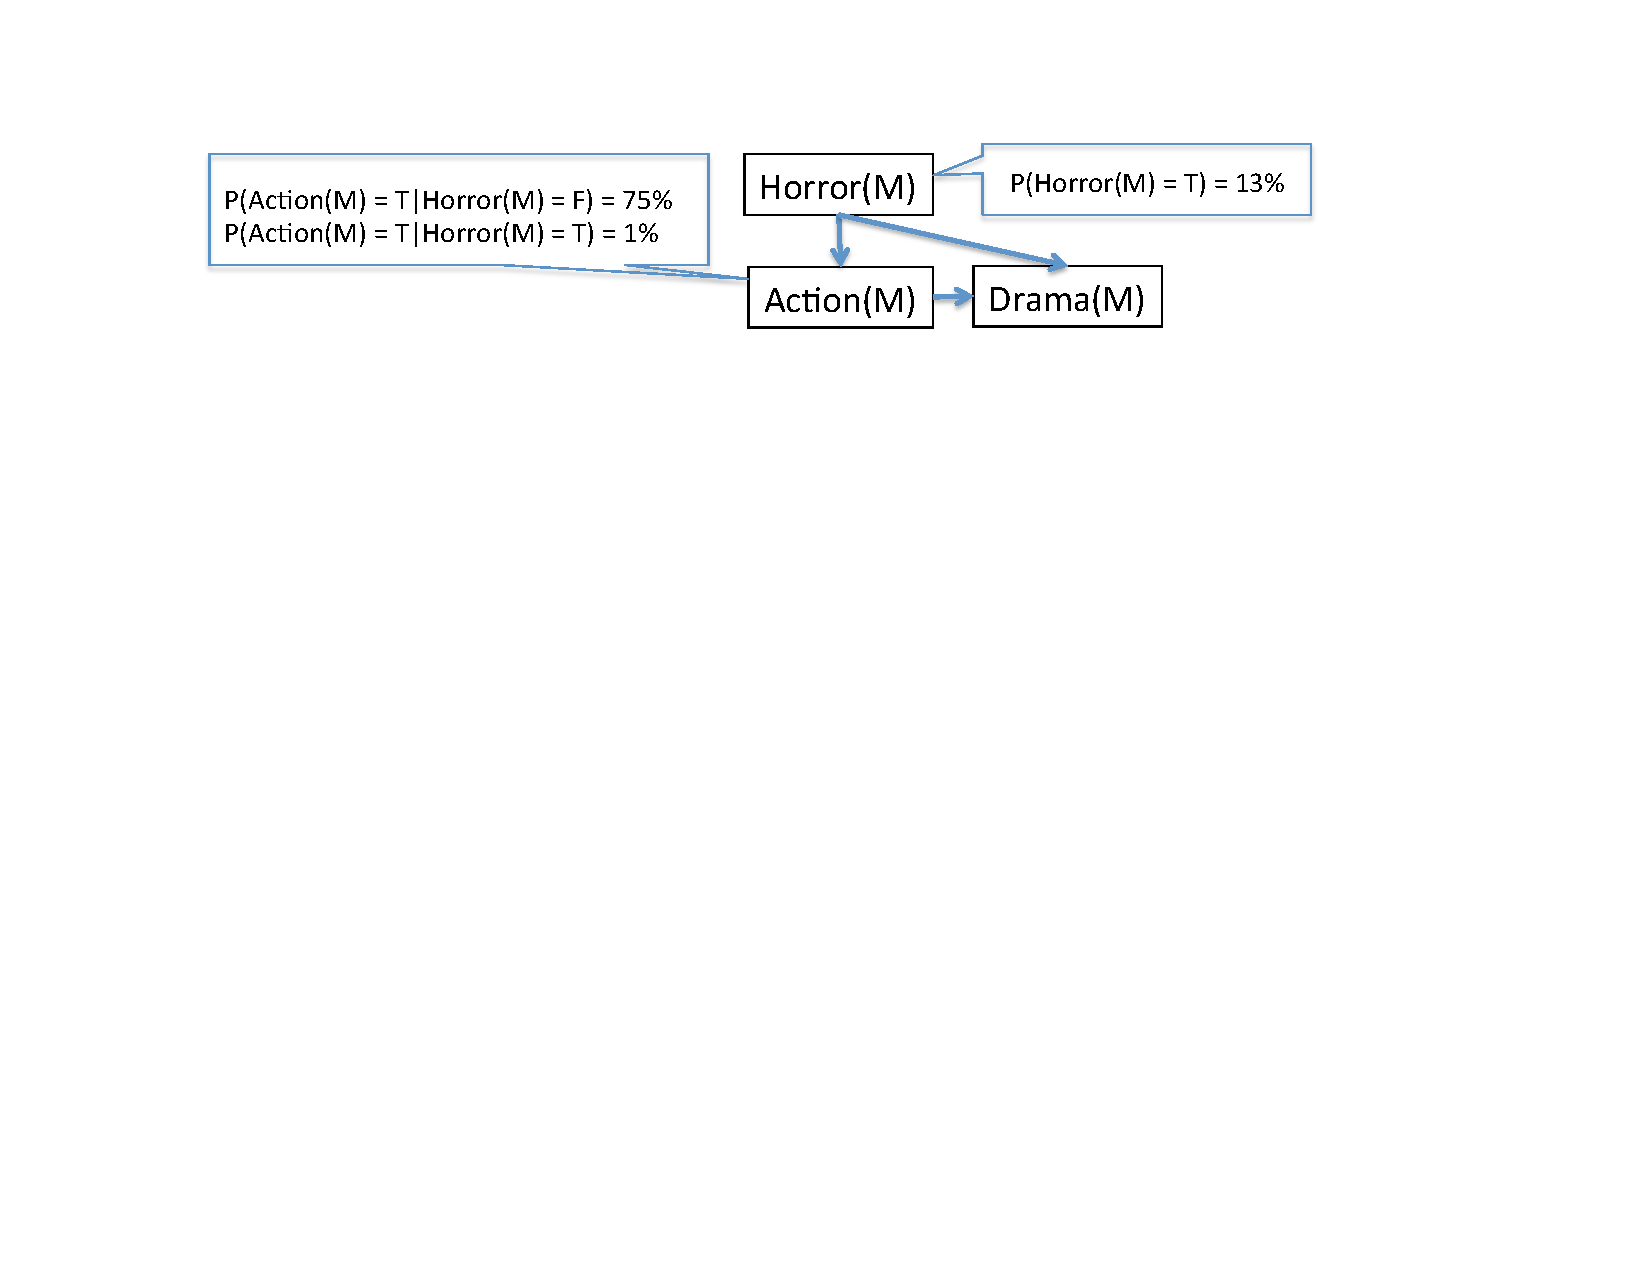
\includegraphics[width=1\textwidth] 
 		{movie-bn2.pdf}
 		\caption[Example of conditional and marginal probabilities computed from a toy Bayesian network structure. ]{The Bayesian network from Figure~\ref{fig:bn-imdb}, where the node names are expanded using the syntax of first-order random variables.
 			\label{fig:bn-imdb2}
 		}
 	\end{figure}


Figure~\ref{fig:bns} shows a first-order Bayesian network for the Premier League domain that is truly relational in that the functors depend on more than one population variable. For example, shot efficiency does not depend on a match only, but also depends on specifying a team. The BN product formula~\eqref{eq:bn} can be applied to any FOBN to compute (estimated) frequencies. In the case of a truly relational FOBN, as in Figure~\ref{fig:bns}, the FOBN can be viewed as representing database frequencies (rather than data table frequencies as in Figure~\ref{fig:bn-imdb2}). Using Getoor's terminology, the FOBN can be viewed as a Statistical-Relational Model (SRM)~\citep{Getoor2001a,Schulte2014,Schulte2017a}.


%\footnote{\textbf{Sarah}: add marginal probability P(res=win) for object parameters}
 	\begin{figure}[t]
 		\centering
 		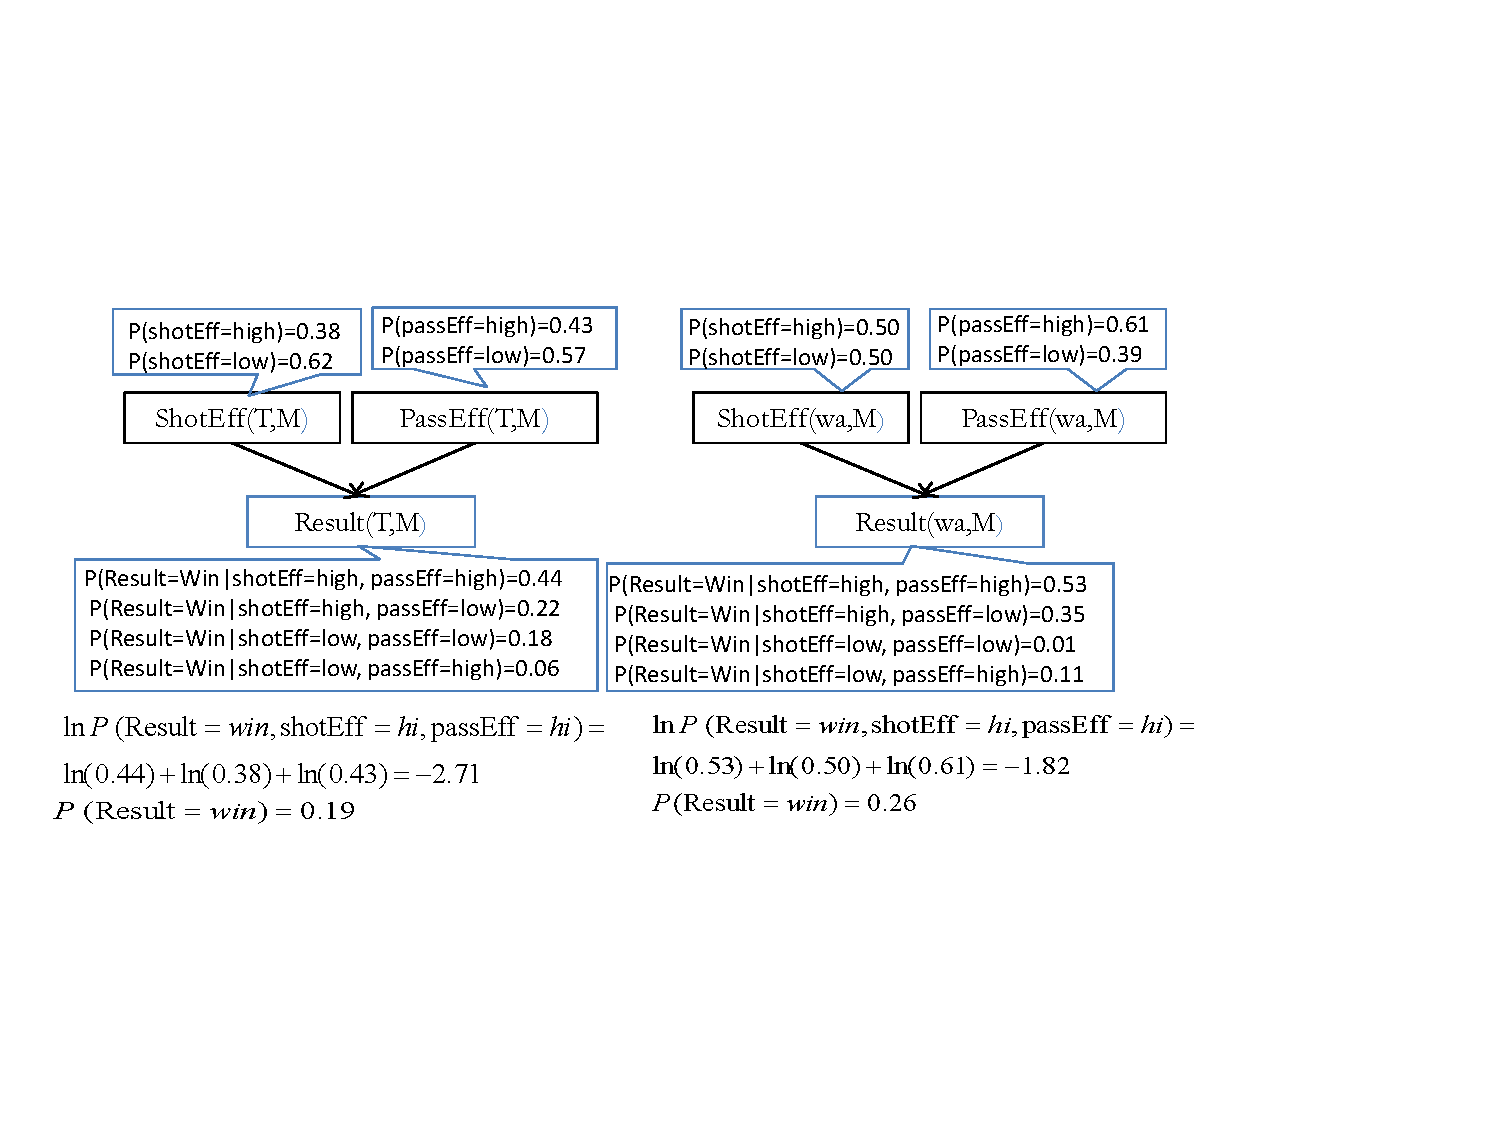
\includegraphics[width=1\textwidth] 
 		{wa.pdf}
 		\caption[Example of joint and marginal probabilities computed from a toy Bayesian network structure. ]{Example of joint and marginal probabilities computed from a toy Bayesian network structure. The parameters were estimated from the  Premier League data set. (left): A class model Bayesian network $\model_{\class}$ for all teams with class parameters $\parameters_{\class}$. The first-order variable $T$ ranges over teams, and the first-order variable $M$ over matches. For compactness, conditional probabilities omit the first-order variables and constants. (right): The same Bayesian network structure with object parameters $\parameters_{\object}$ learned for Wigan Athletic ($T = WA$). 
 			%We show only the Markov blanket of the Results node to simplify. 
 			\label{fig:bns}
 		}
 	\end{figure}
			

	\subsection{Likelihood Score for first-order Bayesian Networks.}\label{sec:log}
	A standard method for applying a generative model assumes that the generative model represents normal behavior since it was learned from the entire population. An object is deemed an outlier if the model assigns sufficiently low likelihood to generating its features \citep{Cansado2008}. This likelihood method is an important baseline for our investigation.
	%so we define the likelihood function formally in this section. 
The other outlierness scores we consider are improved variants of the likelihood approach. 
	Defining a likelihood for relational data is more complicated than for i.i.d. data, because an object is characterized not only by a feature vector, but by an object  database.
	% that lists the object's links and the attributes of linked entities. 
	%For the model likelihood function $\lnlikelihood(\model,\D)$, where $\model$ denotes a Bayesian network, 
	We employ the previously defined normalized relational log-likelihood  score \citep{Schulte2011,Xiang2011}, which can be computed as follows for a given Bayesian network  and database.
	
	%\begin{eqnarray}
	%\lnlikelihood(\model,\D) =   \sum_{i=1}^{n}\sum_{j=1}^{\states_{i}} \sum_{\parents_{i}}\\ P_{\D}(\feature_{i} = \nodevalue_{ij},\parents_{i})\ln \parameter_{\model}(\feature_{i} = \nodevalue_{ij}|\parents_{i})  \nonumber
	%\end{eqnarray}
	
	\begin{equation} \label{eq:likelihood}
		\loglikelihood(\D,\model,\parameters) =   \sum_{i=1}^{n}\sum_{j=1}^{\states_{i}} \sum_{\parents_{i}}\P_{\D}(\nodevalue_{ij},\parents_{i})\ln \parameter(\nodevalue_{ij}|\parents_{i})  
	\end{equation}
	
	
	Equation~\eqref{eq:likelihood} has the same form of the standard BN log-likelihood function for vectorial i.i.d. data~\citep{Campos2006}}, except that parent-child instantiation counts are standardized to be proportions \citep{Schulte2011,Schulte2017a}. For the notation please refer to Table~\ref{table:notation}. The condition under which the score of Equation~\eqref{eq:likelihood} sums to 1 over all relational data sets are discussed in \citep{Schulte2011}.\footnote{Briefly, if the first-order Bayesian Network is viewed as a template for an unrolled ground network, then (1) the ground network cannot contain cycles, and (2) each ground network cannot have multiple parent instantiations; see also \citep{Heckerman+al:SRL07}.}  The equation can be read as follows.
	
	\begin{enumerate}
		\item For each parent-child configuration, 
		use the conditional probability of the child given the parent.
		\item Multiply the logarithm of the conditional probability by the database frequency of the parent-child configuration. 
		%The instantiation proportion is the number of instantiating groundings, divided by the total number of possible instantiations.
		\item Sum this product over all parent-child configurations and all nodes. 
	\end{enumerate}
	
	%\begin{eqnarray}
	%\lnlikelihood&   \sum_{i=1}^{n}\sum_{j=1}^{\states_{i}} \sum_{\parents_{i}} P_{\D}(\feature_{i} = \nodevalue_{ij},\parents_{i})\ln \parameter_{\model}(\feature_{i} = \nodevalue_{ij}|\parents_{i})
	%\end{eqnarray}
	
	The maximum of the relational log-likelihood ~\eqref{eq:likelihood} is given by the empirical database frequencies \cite[Prop.3.1.]{Schulte2011}. In all our experiments we use these maximum likelihood parameter estimates.
	
\paragraph{Example.} Consider the class-level BN of Figure~\ref{fig:bns}(left). The family configuration \begin{displaymath} \it{passEff(T,M)=high}, shotEff(T,M)=high, Result(T,M)=win\end{displaymath} contributes one term to the log-likelihood score For the population database $\D$, this term is 
\begin{eqnarray*}
P_{D}(\it{passEff(T,M)=high}, shotEff(T,M)=high, Result(T,M)=win) &\times&\\ \ln P(Result(T,M)=win|\it{passEff(T,M)=high}, shotEff(T,M)=high)  &=&\\ 0.1 \times \ln(0.44) =-0.08 & &
\end{eqnarray*}
where the database frequency 0.1 is computed as in Table~\ref{table:counts} and the conditional probability 0.44 is the parameter specified by the Bayesian network of Figure~\ref{fig:bns}. 
	
		
	For the  Wigan Athletic data $\D_{WA}$, the corresponding term is 
	\begin{eqnarray*}
P_{\D_{WA}}(\it{passEff(WA,M)=high}, shotEff(WA,M)=high, Result(WA,M)=win) &\times&\\ \ln P(Result(WA,M)=win|\it{passEff(WA,M)=high}, shotEff(WA,M)=high)  &=&\\ 0.18 \times \ln(0.44) =-0.14 & &
\end{eqnarray*}
where the database frequency 0.18 is computed as in Table~\ref{table:counts} and the conditional probability 0.44 is the parameter specified by the Bayesian network of Figure~\ref{fig:bns}(left). 


\section{Exceptional Model Mining for Relational Data} \label{sec:eld}

This section describes our approach to applying the EMM framework to relational data, using the following notation.
%
%In this section, we introduce a novel model-based outlierness score, that extends the relational log-likelihood~\eqref{eq:likelihood}, and outline the steps involved in the score computation.
%\subsection{Computation Flow}  
%We use the following notation to define the computation steps for the relational outlierness scores examined in this paper.
\begin{itemize}
	\item $\D_{\Class}$ is the database for the entire class of objects; cf. Table~\ref{table:data}. This database defines the \textbf{class distribution} $P_{\Class} \equiv P_{\D_{\class}}$.
	\item $\D_{\object}$ is the restriction of the input database to the target object; cf. Table~\ref{table:individual}. This database defines the \textbf{object distribution} $P_{\object} \equiv P_{\D_{\object}}$.
	\item $\model_{\Class}$ is a Bayesian network structure learned with $\D_{\Class}$ as the input database. Note that we use the entire population data to learn the Bayesian network structure. Therefore, the Bayesian network structure is the same across different individuals.
	\item $\parameters_{\Class}$ resp. $\parameters_{\object}$ are parameters learned for $\model_{\Class}$ using $\D_{\class}$ resp. $\D_{\object}$ as the input database.
\end{itemize}

Figure~\ref{fig:flow} illustrates these concepts and the system flow for computing an outlierness score. First, we learn a Bayesian network structure $\model_{\Class}$ for the entire population using a previous learning algorithm (see Section~\ref{sec:methods}). We then compute an {\em outlierness metric} that evaluates how much the object model deviates from the class model. 
%
%\subsection{Definition of Log-Likelihood Distance Outlier Metric} 
%
For a given model type, quantifying the extent to which an object model deviates from the population class model is the main research question in EMM~\citep{Duivesteijn2016}. In this paper we examine several outlierness metrics that are based on the likelihood ratio between the object model and the class model. 
A novel metric that we propose is the \textbf{expected log-likelihood distance} ($\mid$). It is defined as follows for each feature $i$; the total score is the sum of feature-wise scores. Section~\ref{sec:divergence-examples}  provides example computations.


\begin{figure}[htbp]
	\centering
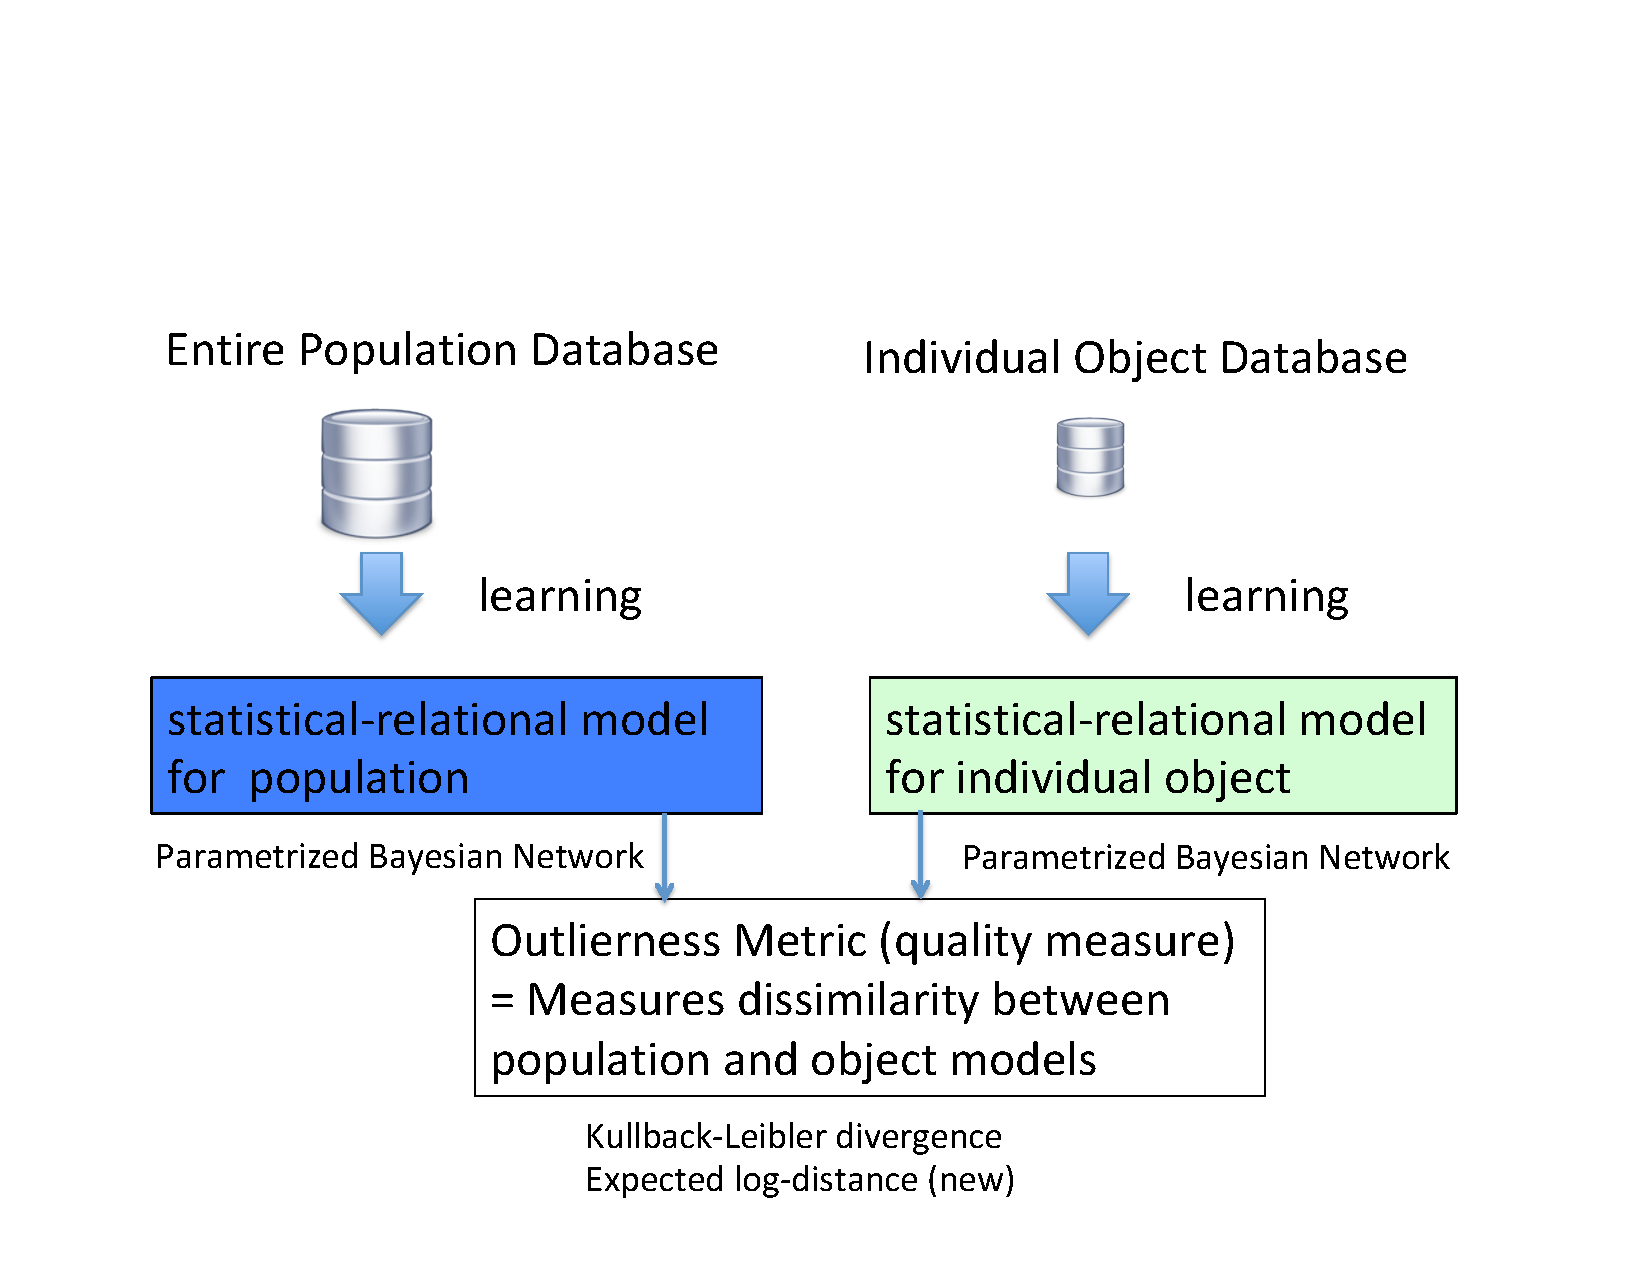
\includegraphics[width=0.8\textwidth]{emm-srl.pdf}
% pdf from SSCI-2015
	\caption{Exceptional model mining for statistical-relational models (cf. Figure~\ref{fig:emm}). The model class we utilize in this paper are first-order Bayesian networks, with a log-linear likelihood function. As outlierness metrics we consider the standard Kullback-Leibler divergence, and the novel divergence $\mid$ described in the text.
		\label{fig:flow}}
\end{figure}


\begin{eqnarray}
\mid_{i} & = & \sum_{j=1}^{\states_{i}} P_{\object}(\nodevalue_{ij}) \left|\ln \frac{\parameter_{\object}( \nodevalue_{ij})}{\parameter_{\Class}( \nodevalue_{ij})}\right|+ \label{eq:fd}\\
& & \sum_{j=1}^{\states_{i}} \sum_{\parents_{i}} 
P_{\object}( \nodevalue_{ij},\parents_{i})
\left|\ln \frac{\parameter_{\object}( \nodevalue_{ij}|\parents_{i})}{\parameter_{\object}(\nodevalue_{ij})} - \ln \frac{\parameter_{\Class}( \nodevalue_{ij}|\parents_{i})}{\parameter_{\Class}(\nodevalue_{ij})}\right|. \label{eq:mi}
\end{eqnarray}

\subsection{Interpretation}

The first sum~\eqref{eq:fd} is the \textbf{single-feature} component, where each feature is considered independently of all others. It computes the expected log-distance with respect to  the single feature value probabilities between the object and the class models. 
%For example, the single-feature sum for the feature ``Goal" of Van Persie is 5/8. 
%
The second $\mid$ sum~\eqref{eq:mi} is the \textbf{mutual information component}, based on the mutual information among all features. It computes the expected log-distance with respect to the mutual information of feature value assignments between the object and the class models.
%measures the expected distance in 
%%{\em multi-variate mutual information} 
%{\em association component} between the object and the class distributions. 
Intuitively, the first sum measures how the models differ if we treat each feature in isolation. The second sum measures how the models differ in terms of how strongly parent and child features are associated with each other. 


\subsection{Motivation} 

The motivation for the mutual information decomposition is two-fold. 
(1) {\em Interpretability.} This is very important for outlier detection. The single-feature components are easy to interpret since they involve no feature interactions. Each parent-child local factor is based on the average relevance of parent values for predicting the value of the child node, where relevance is measured by $$\ln \frac{\parameter(\nodevalue_{ij}|\parents_{i})}{\parameter(\nodevalue_{ij})}.$$ This relevance term  is basically the same as the widely used lift measure \citep{Tuffery2011}, hence is an intuitively meaningful quantity. The $\mid$ score compares how relevant a given parent condition is in the object data with how relevant it is in the general class. 


(2) {\em Avoiding cancellations.} 
For different child-parent configurations, the different components of the $\mid$ sum may have different signs. This leads to a partial cancelling of differences between the class and object distributions. Since our goal is to assess the distinctness of an object, {\em we do not want differences to cancel out.} Taking distances as in Equations~\eqref{eq:fd} and ~\eqref{eq:mi} avoids the undesirable loss of information. 
%The general point is that averaging differences is appropriate when considering costs, or utilities, but not appropriate for assessing the distinctness of an object. In contrast, the absolute values add differences regardless of their sign. 
The next section provides comparison scores and example computations that illustrate the cancelling phenomenon that occurs without adding absolute values. The subsequent section~\ref{sec:theory} provides a Taylor series analysis for a theoretical understanding of the cancelling phenomenon: We show that without the absolute values (as with $\lr$), the first-order term in the Taylor series approximation vanishes, whereas with the absolute values (as with $\eld$), the first-order term is equivalent to the total variation distance (L1 norm). 

\section{Comparison Scores} \label{sec:metrics}

We introduce several alternative likelihood-ratio based outlierness scores, following a lesion design where different scores omit different components of our main $\mid$ proposal. %We introduce the scores. 
To illustrate their essential difference with $\mid$, we give toy examples before we evaluate them on full data sets.

\subsection{Definition of Comparison outlierness scores}

\paragraph{Log-likelihood Ratio Score.} Our first comparison score omits the absolute values from the $\mid$ score: 

\begin{eqnarray*}
\lr_{i} & = & \sum_{j=1}^{\states_{i}} P_{\object}(\nodevalue_{ij}) \ln \frac{\parameter_{\object}( \nodevalue_{ij})}{\parameter_{\Class}( \nodevalue_{ij})}+ \sum_{j=1}^{\states_{i}} \sum_{\parents_{i}} 
P_{\object}( \nodevalue_{ij},\parents_{i})
(\ln \frac{\parameter_{\object}( \nodevalue_{ij}|\parents_{i})}{\parameter_{\object}(\nodevalue_{ij})} - \ln \frac{\parameter_{\Class}( \nodevalue_{ij}|\parents_{i})}{\parameter_{\Class}(\nodevalue_{ij})}).
\end{eqnarray*}

By using the \textbf{mutual information decomposition:}


\begin{equation} \label{eq:decompose}
\ln \frac{\parameter_{\object}( \nodevalue_{ij}|\parents_{i})}{\parameter_{\Class}( \nodevalue_{ij}|\parents_{i})} = \ln \frac{\parameter_{\object}(\nodevalue_{ij}|\parents_{i})}{\parameter_{\object}(\nodevalue_{ij})} - \ln \frac{\parameter_{\Class}( \nodevalue_{ij}|\parents_{i})}{\parameter_{\Class}(\nodevalue_{ij})} + \ln \frac{\parameter_{\object}( \nodevalue_{ij})}{\parameter_{\Class}( \nodevalue_{ij})},
\end{equation}

\noindent it can be shown that the $\mid$ score without the absolute values is equivalent to 
the likelihood ratio, or {\bf log-likelihood difference}:
%. The log-likelihood difference is defined by

\begin{equation} \label{eq:log-diff}
\lr(\D_{\object},\model_{\Class},\parameters_{\object}) \equiv \loglikelihood(\D_{\object},\model_{\Class},\parameters_{\object}) - \loglikelihood(\D_{\object},\model_{\Class},\parameters_{\Class}).
\end{equation}

Assuming maximum likelihood parameter estimation, $\lr$ is equivalent to the Kullback-Leibler divergence between the class-level and object-level parameters~\citep{Campos2006}. The log-likelihood difference compares  how well the class-level parameters fit the object data with respect to a particular object, vs. how well the object parameters fit the object data. It measures how much the log-conditional probabilities in the class distribution differ from those in the object distribution. 
%Note that this definition applies only for relational data where an individual is characterized by a substructure rather than a ``flat'' feature vector. 
%
\paragraph{The Feature Divergence Score.}
The feature divergence outlierness score $\fd$ uses only part~\eqref{eq:fd} of the $\mid$ score. That is, it considers each feature independent of all others.  $\fd$ computes the expected log-distance with respect to  the single feature value probabilities between the object and the class models:
% This can be computed using the following formula:
\begin{equation}
\fd_{i}	=\sum_{i=1}^{n}\sum_{j=1}^{\states_{i}} P_{\object}( \nodevalue_{ij}) \left|\ln \frac{\parameter_{\object}( \nodevalue_{ij})}{\parameter_{\Class}( \nodevalue_{ij})}\right|
\end{equation}


\paragraph{Log-Likelihood Score.} 

In previous work on applying Bayesian networks to outlier detection for i.i.d. non-relational data, the outlier metric used was the log-likelihood of a data point \citep{Cansado2008}. This means that an object was deemed an outlier if the model assigns sufficiently low likelihood to generating its features. For relational data, we use the relational log-likelihood \eqref{eq:likelihood} of the target {\em database}:

\begin{equation} \label{eq:loglikelihood-score}
\loglikelihood(\D_{\object},\model_{\Class},\parameters_{\Class}) =   \sum_{i=1}^{n}\sum_{j=1}^{\states_{i}} \sum_{\parents_{i}}\P_{\D}(\nodevalue_{ij},\parents_{i})\ln \parameter(\nodevalue_{ij}|\parents_{i}).
\end{equation}




\subsection{Score Computation Examples} \label{sec:divergence-examples} 
			
			
			We provide three simple examples with only two variables/features that illustrate the computation of the outlierness scores. They are designed so that outliers and normal objects are easy to distinguish, and so that it is easy to trace the behavior of an outlierness score.
			%The examples also illustrate the concepts of attribute and correlation outlier. 
			The examples therefore serve as thought experiments that bring out some key strengths and weaknesses of the model-based outlierness scores we evaluate. 
			Figure~\ref{fig:synthetic-bns} describes the BN representation of the examples. For intuition, we can think of a soccer setting, where each match assigns a value to each attribute $F_{1}$ and $F_{2}$ for each player. 
			
			\begin{figure*}[htbp]
				\centering
				\resizebox{1\textwidth}{!}{
					\includegraphics%[width=0.3\textwidth] 
					{DistributionBN-bk-aug17.pdf}
				}
				\caption{Illustrative Bayesian networks with two nodes. The networks are not learned from data, but hand-constructed to be plausible for the soccer domain. (a) {\em High Correlation:} Normal individuals exhibit a strong association between their features, outliers no association. Both normals and outliers have a close to uniform distribution over single features.
					% The outlier distribution misses a correlation that is present in the normal population. The single feature distributions are uniform in both distributions. 
				(b) {\em Low Correlation:} Normal individuals exhibit no association between their features, outliers have a strong association. Both normals and outliers have a close to uniform distribution over single features.
					% The outlier object exhibits a correlation that is not present in the normal population. The single attribute distributions are uniform in both distributions.
				(c) {\em Single Attributes:} Both normal and outlier individuals exhibit a strong association between their features. In normals, 90\% of the time, feature 1 has value 1. For outliers, feature 1 has value 1 only 10\% of the time. 
					%Correlations are the same, but the single feature distributions are not.
					\label{fig:synthetic-bns}}
			\end{figure*}
			
			

%\paragraph{Example Computations.} 
%\footnote{\textbf{Sarah}:caption sizes are funny}


\begin{table}[hbpt]
	\caption{Example computation of different outlierness scores for outliers given the distributions of Figure~\ref{fig:synthetic-bns}(a),(b). Our new $\eld$ metric contains no negative terms due to the use of absolute values.
	\label{table:example}}
	
	%\captionsetup[table]{skip=10pt}
	
	\centering
	\resizebox{1\textwidth}{!}{
		\begin{tabular}{lp{3cm}p{6cm}l}
			\hline
			Score&$F1=1$ Computation&$F2|F1=1$ Computation&Result\\ \hline
			$\lr$&\begin{tabular}{p{5cm}} $1/2 \ln(0.5/0.5)=0 $\end{tabular}&$1/4\ln(0.5/0.9)+ 1/4\ln(0.5/0.1)$&0.36\\ \hline
			%$ELD$&$1/2|\ln(0.5/0.5)|=0$&$1/4|\ln(0.5/0.9)|+1/4|\ln(0.5/0.1)|$&0.79\\ \hline
		%	$|\lr|$&$0$ (no parents)&\begin{tabular}{p{5cm}}$1/4 |\ln(0.5/0.9)|+1/4|\ln(0.5/0.1)|$\end{tabular}&0.79\\ \hline
			$\fd$&$|\ln(0.5/0.5)|=0$&\begin{tabular}{p{5.5cm}}$1/2|\ln(0.5/0.5)| + 1/2|\ln(0.5/0.5)|$\end{tabular}&0\\ \hline
			%$$\mid$$&$0+0$&$0.79+0$&0.79
			$\mid$&$0$ (no parents)&\begin{tabular}{p{5cm}}$1/2|\ln(0.5/0.5)| + 1/2|\ln(0.5/0.5)| + 
1/4 |\ln(0.5/0.5)-\ln(0.9/0.5)|+1/4 |\ln(0.5/0.5)-\ln(0.1/0.5)|$\end{tabular}&0.79
			
			%$1/4(|\ln(0.9/0.5)-\ln(0.5/0.5)|+|\ln(0.1/0.5)-\ln(0.5/0.5)|+2|\ln(0.5/0.5)|)=0.54$
			\\ \hline
		\end{tabular}}
		%\centering
		\resizebox{1\textwidth}{!}{
			\begin{tabular}{p{11cm}}
				Table 5(a): High Correlation Case, following Figure~\ref{fig:synthetic-bns}(a).
				%: The scores for the object and class BNs of Figure~\ref{fig:synthetic-bns}(a).
				
			\end{tabular}}
			
			%
			\centering
			\resizebox{1\textwidth}{!}{
				\begin{tabular}{lp{3cm}p{6cm}l}
					\hline
					Score&$F1=1$ Computation&$F2|F1=1$ Computation&Result\\ \hline
					$\lr$&$1/2\ln(0.5/0.5)=0$&$0.5 \cdot 0.9 \ln(0.9/0.5)+ 0.5 \cdot 0.1 \ln(0.1/0.5)$&0.26\\ \hline
					%$ELD$&$1/2|\ln(0.5/0.5)=0|$&$0.5 \cdot 0.9|\ln(0.9/0.5)|+0.5 \cdot 0.1|\ln(0.1/0.5)|$&0.50\\ \hline
					%$|\lr|$&$0$ (no parents) &$0.5 \cdot 0.9 |\ln(0.9/0.5)|+ 0.5 \cdot 0.1 |\ln(0.1/0.5)| $&0.50\\ \hline
					$\fd$&$|\ln(0.5/0.5)|=0$&$1/2|\ln(0.5/0.5)| + 1/2|\ln(0.5/0.5)|$&0\\ \hline
					%$\mid$&$0+0$&$0.5+0$&0.5\\ \hline
						$\mid$&$0$ (no parents) &\begin{tabular}{p{5.5cm}}$1/2|\ln(0.5/0.5)| +1/2|\ln(0.5/0.5)| + 0.5 \cdot 0.9 |\ln(0.9/0.5)-\ln(0.5/0.5)|+ 0.5 \cdot 0.1 |\ln(0.1/0.5)-\ln(0.5/0.5)|
						$\end{tabular}&0.50\\ \hline
				\end{tabular}}
				\resizebox{1\textwidth}{!}{
					\begin{tabular}{p{11cm}}
						Table 5(b): Low Correlation Case, following Figure~\ref{fig:synthetic-bns}(b).
						%The scores for the object and class BNs of Figure~\ref{fig:synthetic-bns}(b). 
						
					\end{tabular}}
				\end{table}
				
			

%\subsection{Comparison on Examples}


%
%The single feature distributions are uniform, so the feature component~\eqref{eq:fd} 
%is 0 for each node in both examples.
% 
Table~\ref{table:example} illustrates the computation of the scores. Scores for the $F_{2}$ feature are computed conditional on $F_{1} = 1$. Expectation terms are computed first for $F_{2} = 1$, then $F_{2} = 0$.
The table shows the %undesirable 
cancelling effects in $\lr$. In the high correlation scenario~\ref{fig:synthetic-bns}(a), the outlier object has a lower probability than the normal class distribution of $\it{Match\_Result} = 0$ given that $\it{Shot\_Efficiency} = 1$. Specifically, 0.5 vs. 0.9. The outlier object exhibits a higher probability $\it{Match\_Result} = 1$ than the normal class distribution, conditional on $\it{Shot\_Efficiency} = 1$; specifically, 0.5 vs. 0.1. In line 1, column 2 of Table~\ref{table:example}  the log-ratios $\ln(0.5/0.9)$ and $\ln(0.5/0.1)$ therefore have different signs. In the low correlation scenario~\ref{fig:synthetic-bns}(b), the cancelling occurs in the same way, but with the normal and outlier probabilities reversed. 
The cancelling effect is even stronger for attributes with more than two possible values.

While log-likelihood $\loglikelihood$ is a good baseline score for detecting outliers, it fails to detect some clear outliers, as shown in Figure~\ref{fig:logfails}. In that example the strength of the correlation among the attributes is the same in both normal and outlier examples and the only difference is in their feature distributions.

		\begin{figure*}[htbp]
			\centering
			\resizebox{0.9\textwidth}{!}{
				\includegraphics%[width=0.3\textwidth] 
				{logfails.pdf}
			}
			\caption{An example of normal and outlier individuals and their conditional probability tables created using the Bayesian network shown in Figure~\ref{fig:synthetic-bns}(c). Log-likelihood assigns the same score to the normal and individuals in this example, while $\it{FD}$ is able to differentiate between these two individuals.
				%Correlations are the same, but the single feature distributions are not.
				\label{fig:logfails}}
		\end{figure*}
		



%\subsection{Visualization}\label{sec:visual}
%	
%We generated three synthetic data sets with normal and outlier players using the distributions represented in the three Bayesian networks of Figure~\ref{fig:synthetic-bns}. The main goal of designing synthetic experiments is to test the methods on  easy to detect outliers. We provide a 1D scatter plot for each outlier method to visualize the scores assigned to each player. We used the $\it{mlbench}$ package in $\it{R}$ to generate synthetic features in matches, following these distributions for 240 normal players and 40 outliers. (There were 280 players in our Premier League data set.) Each player participates in 38 matches, similar to the real-world data. Each match assigns a value to each feature $F_i, i =  1,2$ for each player. This design yields the following three synthetic data sets. 
%				\begin{description}
%					\item\textbf{High Correlation} See Figure~\ref{fig:synthetic-bns}(a).
%					\item\textbf{Low Correlation} See Figure~\ref{fig:synthetic-bns}(b).
%					\item\textbf{Single features} See Figure~\ref{fig:synthetic-bns}(c).
%				\end{description}
%				
%Figure~\ref{fig:1DPlots} provides scatter plots for each synthetic data set and each comparison outlier metric. The figure is best viewed on screen. As entailed by Proposition~\ref{prop:divergence}(Part \ref{clause:inequalities}), the $\mid$ metric maps players to the largest range of outlierness scores. It also provides the best separation of normal from abnormal players: The normal players receive low anomaly scores and hence are clustered to the left of the $\mid$ scatter plot, whereas the abnormal players receive high scores and hence are clustered on the right. The $|\lr|$ metric  also shows a larger range of scores and a better discrimination compared to the $\lr$ metric. This illustrates the value of using distances rather than differences. In Section~\ref{sec:detection} we provide an aggregate detection accuracy score that quantifies this values.
%

%
%	\begin{figure}
%		\centering     %%% not \center
%		\subfigure[Distribution of different outlierness scores in Synthetic Dataset- Single Feature. ]{\label{fig:Feature}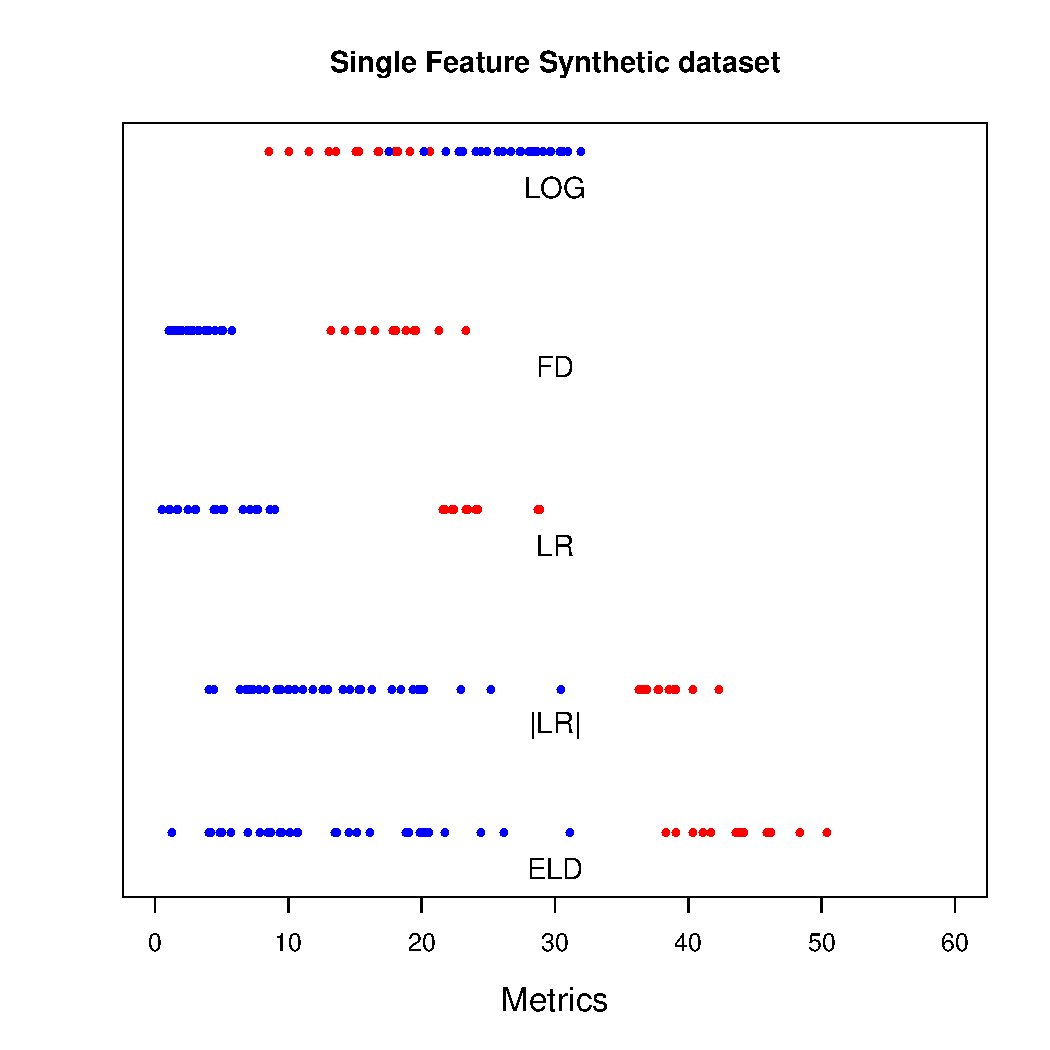
\includegraphics[width=0.48\textwidth]{DistributionPlots/sumFeature-bk-feb2016.pdf}}
%		\subfigure[Distribution of different outlierness scores in Synthetic Dataset- Low correlation]{\label{fig:LowCor}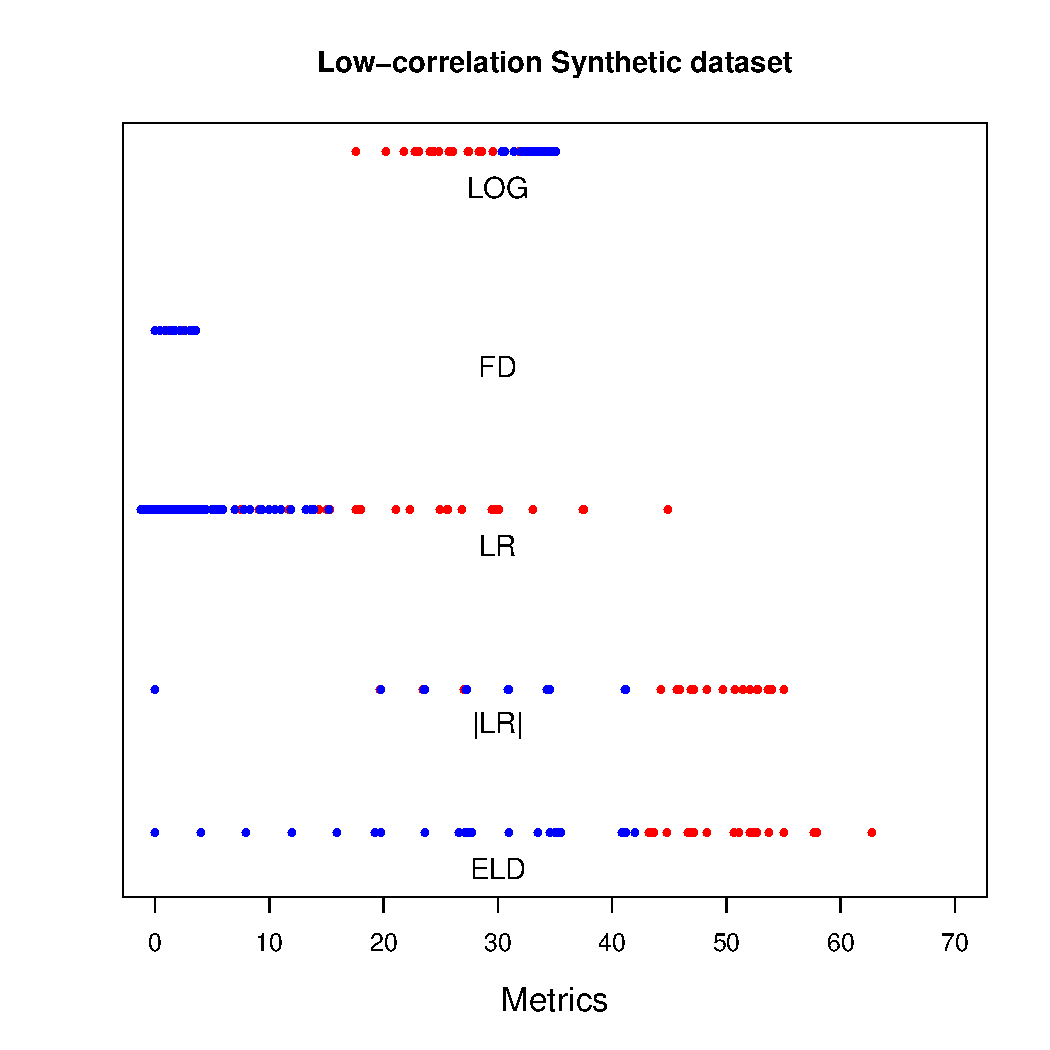
\includegraphics[width=0.5\textwidth]{DistributionPlots/sumSep-bk-feb2016.pdf}}
%		\subfigure[Distribution of different outlierness scores in Synthetic Dataset- High correlation]{\label{fig:HighCor}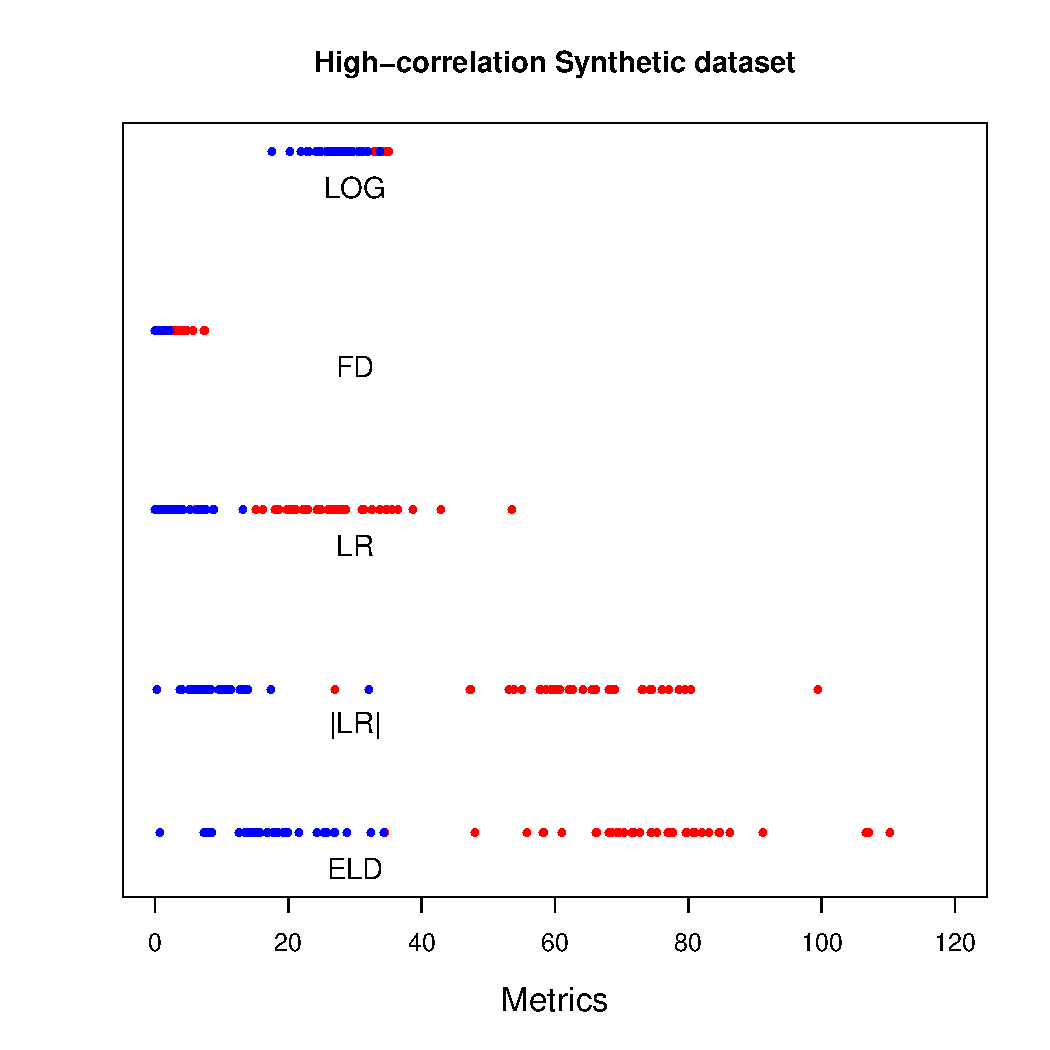
\includegraphics[width=0.5\textwidth]{DistributionPlots/sumSV-bk-feb2016.pdf}}
%		\caption{Visualizing likelihood-based outlier metrics on our three synthetic data sets. The figure is best viewed on the screen. Score values are shown on the $x$-axis; higher values should indicate more anomalous players. For each data set and each metric, we provide a 1D scatterplot of the 280 synthetic player scores. In the scatterplot, blue dots represent normal players, and red dots represent anomalous players.}\label{fig:1DPlots}
%	\end{figure}
%\section{Feature Divergence Object outlierness score}\label{sec:fd}

\begin{figure*}[htbp]
	\centering
	\resizebox{0.9\textwidth}{!}{
		\includegraphics%[width=0.3\textwidth] 
		{fdfails.pdf}
	}
	\caption{An example of normal and outlier individuals and  their conditional probability tables  created using Bayesian network shown in Figure~\ref{fig:synthetic-bns}(a). FD assigns the same score to the normal and individuals in this example, while $\it{LR}$ is able to differentiate between these two individuals.
		%Correlations are the same, but the single feature distributions are not.
		\label{fig:fdfails}}
\end{figure*}
Conversely, if there is a correlation among the attributes of individuals, the feature divergence score $\fd$ fails to take it into account and therefore fails to differentiate between normal and outlier individuals. Figure~\ref{fig:fdfails} shows an example where the normal individual has a correlation among its attributes while the outlier object does not have a correlation. The $\textit{FD}$ metric cannot separate  those two individuals.

\section{Theoretical Analysis and Comparison} \label{sec:theory}

The mathematical analysis of this section relates the $KLD$ and $\mid$ divergences defined in the above sections to other well-known scores. Readers who wish to proceed to the empirical evaluation can omit this section without loss of continuity. 

A well-known Taylor series argument shows that KLD can be approximated by Pearson's $\chi^{2}$ statistic \citep{Nielsen2014}. We use a similar Taylor series approximation to compare our ELD divergence with other divergences such as KLD. The analysis shows that the dominant component of ELD is the total variation distance (TVD), also known as the L1-norm, whose statistical properties are well understood~\citep{Beirlant2001,Beirlant1994}. 
%The Taylor series approximation provides a clear explanation of the cancellation phenomenon: For KLD and $\chi^{2}$, the first-order term in the Taylor series vanishes, whereas for ELD and TVD it does not. 

Our analysis uses the $f$-divergence framework, which unifies all the standard divergence definitions for probability distributions. The $f$-divergence analysis shows the generality of the cancellation phenomenon: the first-order Taylor series term vanishes for all $f$-divergences whose generator $f$ is differentiable at $\lambda = 1$, which includes all standard $f$-divergences (including KLD), except for those that use absolute values. 

\paragraph{The $\chi^2$ approximation for $f$-divergences.}
To focus the mathematics on the essential insights, we discuss the case of divergences defined over a single discrete random variable $\feature$ with possible values $\nodevalue_{1},\ldots,\nodevalue_{m}$. The results carry over to the joint BN distributions over discrete variables considered in this paper, by applying the approximation to each parent state. Given two probability distributions $P_{1}$ and $P_{2}$ over the values of $\feature$, an $f$-divergence is of the form 

\begin{equation}
\label{eq:f-divergence}
I_{f}(P_{1}||P_{2}) \equiv \sum_{i=1}^{m} P_{1}(\nodevalue_{i}) f\left(\frac{P_{2}(\nodevalue_{i})}{P_{1}(\nodevalue_{i})}\right)
\end{equation}
%
where the \textbf{generator} $f:R \rightarrow R$ is a convex function such that $f(1)=0$. 
The generator transforms the ratio of the two compared probabilities for each possible value; the $f$-divergence is the weighted average of the transformed ratios. Common divergences can be represented by choosing a suitable generator. For example, KLD is generated by $f(u) = -\ln(u)$, the $\chi^{2}$ statistic by $f(u) = (1-u)^{2}/u$, and the TVD by $f(u) = |u-1|$ \citep{Nielsen2014}. 

An $f$-divergence $I_{f}$ can be approximated by  replacing $f$ with its Taylor series expansion around the point $u=1$. Assuming that the derivatives $f^{(i)}(1)$ of any order exist, the Taylor series for $f$ takes the form 

 $$f(u) = \sum_{l=0}^{\infty} \frac{f^{(l)}(1)}{l!} [u-1]^{l},$$ where the $l=0$ term is 0 because $f(1) = 0$. Substituting the Taylor series expansion into the $f$-divergence expression~\eqref{eq:f-divergence}  yields an $f$-divergence expansion, {\em assuming that all derivatives of $f$ exist}:
 
\begin{equation*} \label{eq:f-taylor-series}
I_{f}(P_{1}||P_{2}) = \sum_{l=0}^{\infty} \frac{f^{l}(1)}{l!} \sum_{i=1}^{m} 
\frac{[P_{2}(\nodevalue_{i}) - P_{1}(\nodevalue_{i})]^{l}}
{P_{1}(\nodevalue_{i})^{l-1}}.
\end{equation*}

A detailed derivation is in the appendix. Equation~\eqref{eq:f-taylor-series} shows that if the generator $f$ is infinitely differentiable, the $f$-divergence is a series of $l$-metrics, scaled by the derivates and by the $P_1$ probabilities. For statistical applications, usually a second-order expansion up to $l=2$ provides a sufficiently close approximation. If the generator $f$ is twice differentiable, the first-order term with $i=1$ vanishes, and the remaining second-order term with $i=2$ is a scaled $\chi^{2}$ statistic \citep{Nielsen2014}:

\begin{proposition}[Nielsen and Nock 2014] \label{prop:xi-square}
Assume that the generator $f$ for $I_{f}$ is twice differentiable.   

\begin{enumerate}
\item The $i=1$ Taylor series term for  $I_{f}$ around $u=1$ is 0.
\item The $i=2$ Taylor series term for  $I_{f}$ around $u=1$ is a scaled $\chi^{2}$ divergence.
\end{enumerate}

Therefore the second-order Taylor series approximation to $I_{f}$ is scaled $\chi^{2}$-divergence:

$$I_{f}(P_{1}||P_{2}) \approx \frac{f''(1)}{2} \chi^{2}(P_{1}||P_{2}) = \frac{f''(1)}{2} 
\sum_{i=1}^{m}  \frac{(P_{2}(\nodevalue_{i})-P_{1}(\nodevalue_{i}))^{2}}
 {P_{1}(\nodevalue_{i})}.$$ 
\end{proposition} 

{\em Proof Outline.} 
The first-order term reduces to $f'(1) [\sum_{i=1}^{m} P_{2}(\nodevalue_{i}) - \sum_{i=1}^{m} P_{1}(\nodevalue_{i})]$, which vanishes because both probability measures sum to 1. The second-order term reduces to $ \frac{f''(1)}{2} \chi^{2}(P_{1}||P_{2})$. The details are given in the Appendix. 

The first clause provides a clear formulation of the cancelling phenomenon discussed in Section~\ref{sec:divergence-examples}: the first-order terms cancel out exactly.


\paragraph{The Taylor series approximation for $\eld$.}

Our ELD metric is an example of transforming an $f$-divergence with absolute values by replacing the generator $f$ with $|f|$; in our case, replacing $-\ln(u)$ by $|-ln(u)|$ (cf. Equation~\eqref{eq:log-diff}). Because $|x|$ is not differentiable at 0,  the absolute value generator $|f|$ is generally not differentiable at $u=1$, so Proposition~\ref{prop:xi-square} does not apply. To utilize Taylor series analysis, we can rewrite the absolute value divergence as a positive sum where $f(u)>0$ and a negative sum where $f(u) < 0$. 

\begin{equation*} \label{eq:f-absolute}
I_{|f|}(P_{1}||P_{2}) \equiv \sum_{i:f(\frac{P_{2}(\nodevalue_{i})}{P_{1}(\nodevalue_{i})})>0} P_{1}(\nodevalue_{1}) f\left(\frac{P_{2}(\nodevalue_{i})}{P_{1}(\nodevalue_{i})}\right) - \sum_{i:f(\frac{P_{2}(\nodevalue_{i})}{P_{1}(\nodevalue_{i})})<0} P_{1}(\nodevalue_{1}) f\left(\frac{P_{2}(\nodevalue_{i})}{P_{1}(\nodevalue_{i})}\right)
\end{equation*}

In the Taylor series approximation for $\mid$ (using $f=-\ln(u)$ in Equation~\eqref{eq:f-absolute}), cancellation is avoided, so the first-order term does {\em not} vanish, and is in fact equivalent to the Total Variation Distance. The second-order term is equivalent to the \textbf{cancelled $\chi^2$ metric}, which we define as 

\begin{equation*}
\overline{\chi}^2(P_{1}||P_{2}) \equiv 1/2 
\sum_{i:P_{2}(\nodevalue_{i}) < P_{1}(\nodevalue_{i})} [P_{2}(\nodevalue_{i}-P_{1}(\nodevalue_{i}]^2/P_{1}(\nodevalue_{i}) - 
1/2 \sum_{i:P_{2}(\nodevalue_{i}) > P_{1}(\nodevalue_{i})} [P_{2}(\nodevalue_{i}-P_{1}(\nodevalue_{i}]^2/P_{1}(\nodevalue_{i})
\end{equation*}


\begin{proposition} Consider the Taylor series approximation for  $\mid$ around $u=1$ with generator $|f|=|-ln(u)|$. 
\begin{enumerate}
\item The $i=1$ Taylor series term is is total variation distance:
$$\mid(P_{1}||P_{2}) \approx  \TVD =  \sum_{i} |P_{2}(\nodevalue_{i})-P_{1}(\nodevalue_{i})|$$
\item The $i=2$ Taylor series term for  $I_{f}$ around $u=1$ is the cancelled $\overline{\chi}^2(P_{1}||P_{2})$ divergence.
\end{enumerate}
\end{proposition}

In summary, a second-order Taylor series expansion shows that, up to constant factors, divergences can be approximated as first-order term corresponding to total variation distance (TVD), also known as the L1-norm, plus a second-order term corresponding to a $\chi^{2}$ divergence. Cancellation occurs depending on the sign of the probability differences $P_1(v_i) - P_2(v_i)$: differences with opposing signs can cancel out. In KLD, complete cancellation occurs with the first-order term, so the L1-component vanishes. In our absolute value metric ELD, no first-order term is cancelled, but some second-order terms cancel, so the magnitude of the $\chi^{2}$ is diminished. 


%
%
%Therefore 
%the first-order Taylor series approximation for $\mid$ is total variation distance:
%$$\mid(P_{1}||P_{2}) \approx  \TVD =  \sum_{i} |P_{2}(\nodevalue_{i})-P_{1}(\nodevalue_{i})|$$
%




%
%				\begin{figure}
%				\caption{Visualizing likelihood-based outlier metrics on our three synthetic data sets. Score values are shown on the $x$-axis; higher values should indicate more anomalous players. For each data set and each metric, we provide a 1D scatterplot of the 280 synthetic player scores. In the scatterplot, empty circles represent normal players, and stars represent anomalous players.}
%				\label{fig:1d}
%									\centering
%									\begin{minipage}{0.45\linewidth}
%										\centering
%										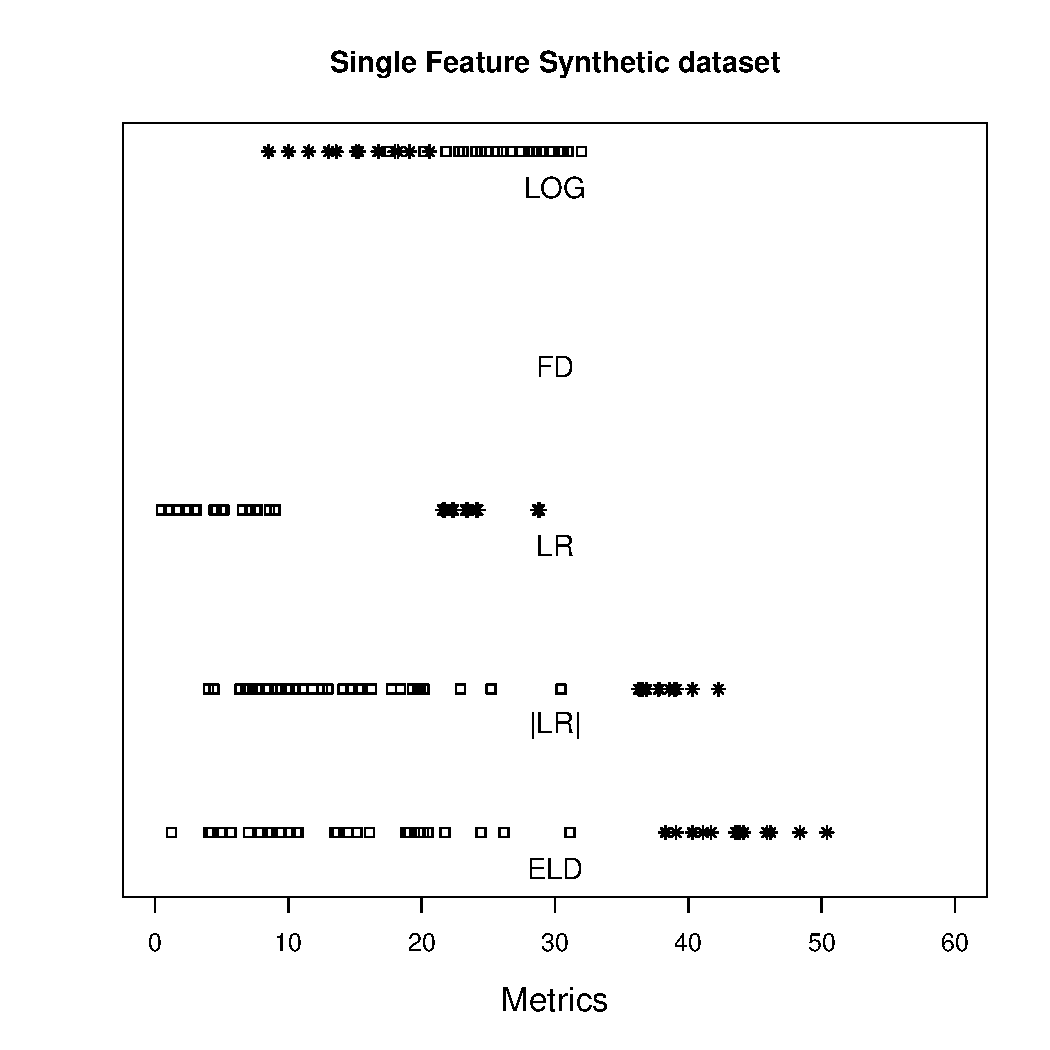
\includegraphics[width=2.5in]{DistributionPlots/sumFeature-bk.pdf}
%										\caption{Distribution of different outlierness scores in Synthetic Dataset- Single Feature. \textbf{what happened to FD?}}
%										\label{fig:StrikerSalary}
%									\end{minipage}
%									\hspace{0.05\linewidth}
%									\begin{minipage}{0.45\linewidth}
%										\centering
%										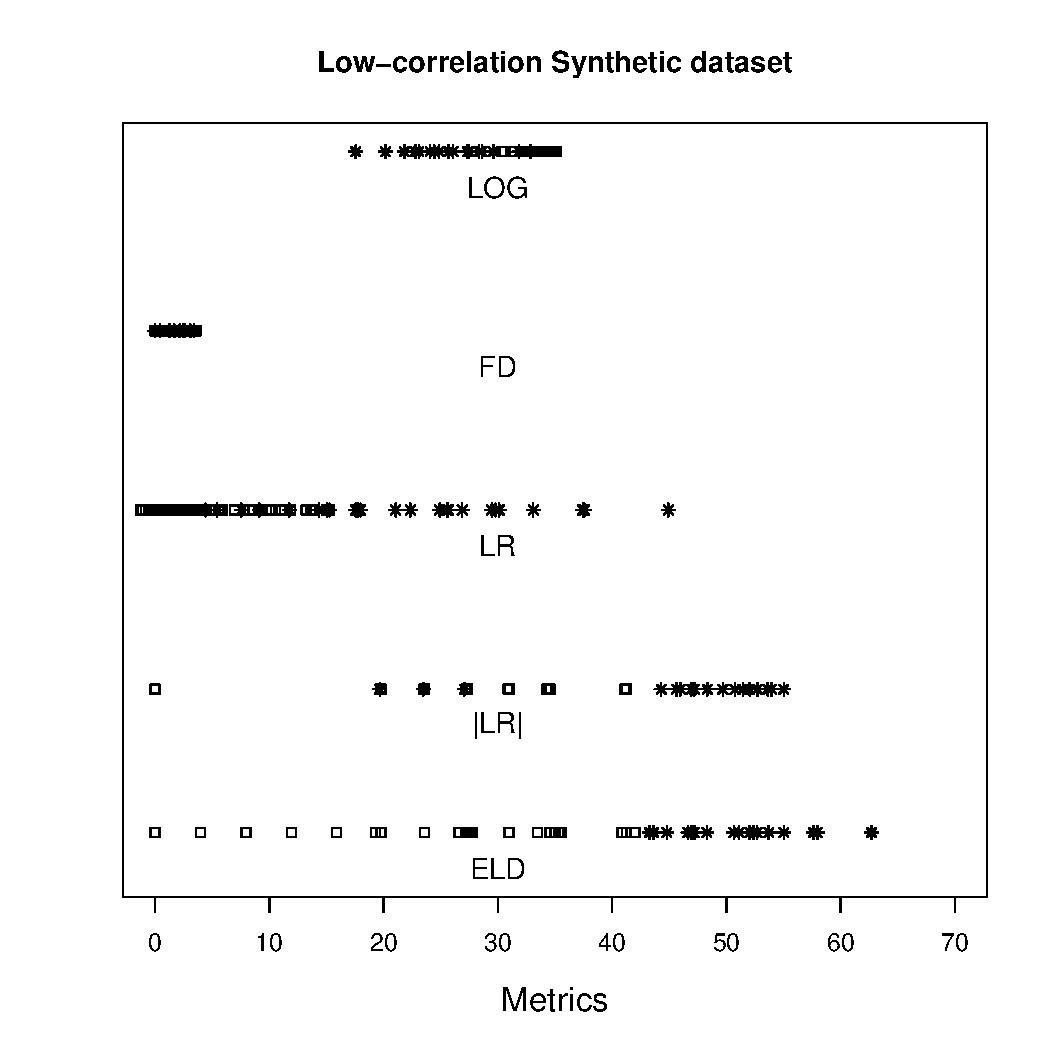
\includegraphics[width=2.5in]{DistributionPlots/sumSep-bk.pdf}
%										\caption{Distribution of different outlierness scores in Synthetic Dataset- Low correlation}
%										\label{fig:StrikerShot}
%									\end{minipage}
%									\hspace{0.05\linewidth}
%									\begin{minipage}{0.45\linewidth}
%										\centering
%										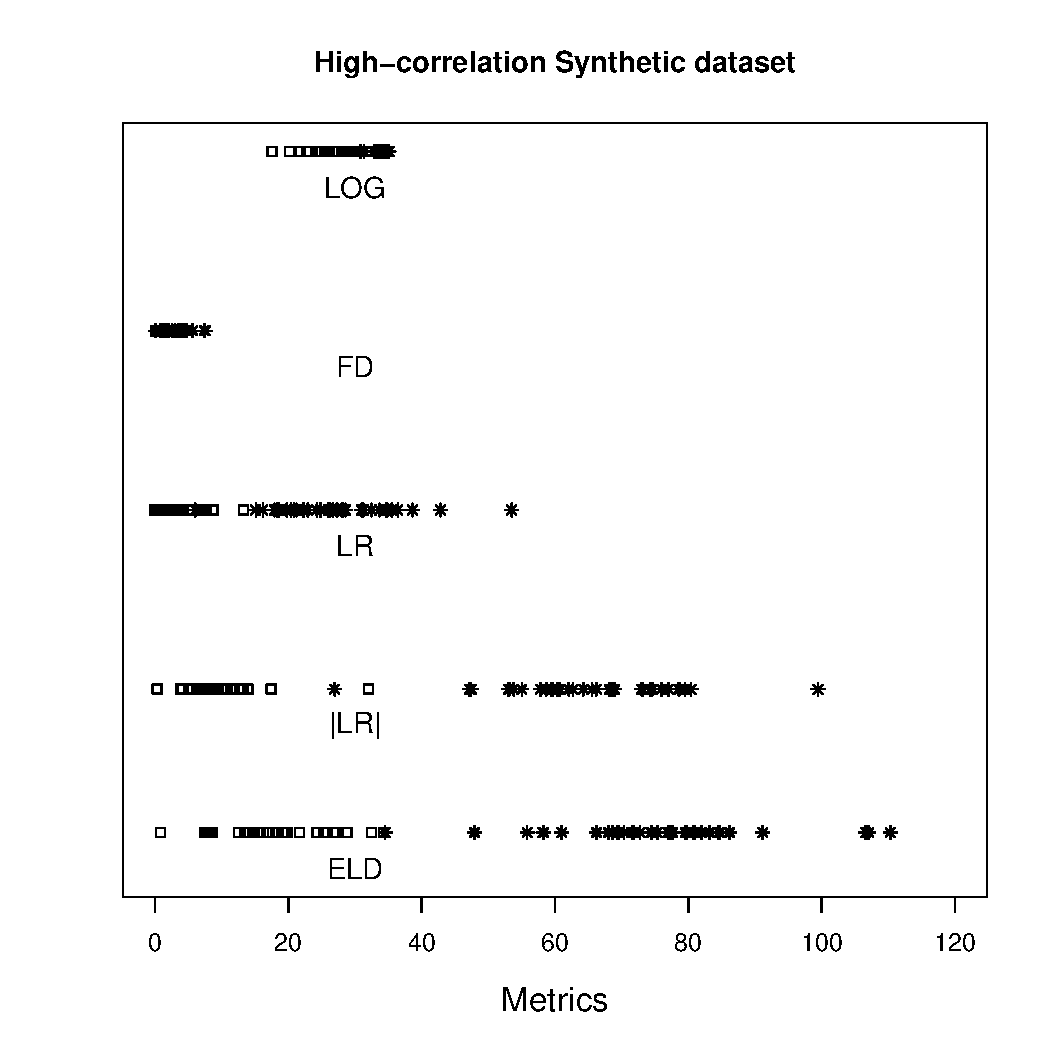
\includegraphics[width=2.5in]{DistributionPlots/sumSV-bk.pdf}
%										\caption{Distribution of different outlierness scores in Synthetic Dataset- High correlation}
%										\label{fig:StrikerTime}
%									\end{minipage}
%								\end{figure}
%				
%				
%				
				
				

				
				
				%The advantages of succinctness and interpretability obtain also for computing scores. We write $B_{\object}$ for a BN that represents the object distribution, and $B_{\Class}$ for a BN that represents the class distribution. Then $\lr$ can be decomposed as $\lr = \sum_{i =1} ^{n} \lr_{i}$, where $$\lr_{i} = \sum_{j=1}^{\states_{i}} \sum_{\parents_{i}} \ln \frac{P_{B_{\object}}(\feature_{i} = \nodevalue_{ij}|\parents_{i})}{P_{B_{\Class}}(\feature_{i} = \nodevalue_{ij}|\parents_{i})}$$ where $\parents_{i}$ indexes all possible parent value combinations for node $\feature_{i}$, and the $P_{B}$ terms denote the conditional probability parameters of the applicable Bayesian network. In words, we sum over all possible child-parent states, and compute the log-probability ratio of the object and class conditional probabilities. The Bayesian network decompositions for the other scores are as follows. We compute feature score as before directly from the class and object distributions, rather than the Bayesian networks, since it concerns only marginal single-feature probabilities. 
				
				%\begin{eqnarray*} 
				%%\tag{$\lr(P_{\object}||P_{\Class})$} 
				%\eld_{i} & = & \sum_{j=1}^{\states_{i}} \sum_{\parents_{i}} |\ln \frac{P_{B_{\object}}(\feature_{i} = \nodevalue_{ij}|\parents_{i})}{P_{B_{\Class}}(\feature_{i} = \nodevalue_{ij}|\parents_{i})}|\\
				%\jid_{i} & = & \sum_{j=1}^{\states_{i}} \sum_{\parents_{i}} |\ln \frac{P_{B_{\object}}(\feature_{i} = \nodevalue_{ij}|\parents_{i})}{P_{\object}(\feature_{i})=\nodevalue_{ij}} - \ln \frac{P_{B_{\Class}}(\feature_{i} = \nodevalue_{ij}|\parents_{i})}{P_{\Class}(\feature_{i})=\nodevalue_{ij}}|\\
				%\mid_{i} & = &
				%\label{eq:eld}
				%\end{eqnarray*}
				
				
				
				
				
				%The learning algorithms were executed with 64-bit Centos with 4GB RAM and an Intel Core i5-480 M processor. 
				
				
				
				%\subsection{Outlier Metrics Compared}
				
				%\begin{description} 
				%We evaluate the outlierness scores $\mid,\eld,\lr$ described in Section~\ref{sec:divergences}. 
				%
				%We use two existing baseline methods. 
				
				%\paragraph{Likelihood Method.} 
				%The metric $\lnlikelihood$ is defined by the equation:
				
				%\begin{equation*} \label{eq:ll}
				%\lnlikelihood_{i} = \sum_{j=1}^{\states_{i}} \sum_{\parents_{i}} P_{\object}(\feature_{i} = \nodevalue_{ij},%\parents_{i})\ln P_{\Class}(\feature_{i} = \nodevalue_{ij}|\parents_{i})
				%\end{equation*}
				
				%The intuition behind this metric is that the class distribution Bayesian network represents normal behavior\cite%{riahi2013}. An object is deemed an outlier if  the class BN assigns sufficiently low likelihood to generating %its features. Using low model likelihood to identify outliers is a common application of Bayesian networks \cite%{Cansado2008a}.  The equation above represents the standard BN log-likelihood function for the object data, %except that parent-child instantiation counts are standardized to be proportions. 
				%This avoids giving exponentially more influence to features with more groundings \citep{Schulte2011}. 
				
				
				%\item[\mid] The outlier metric is the Mutual Information Distance defined in Equation \eqref{eq:mid}. 
				%
				%\item[\eld] The outlier metric is the Mutual Information Distance defined in Equation \eqref{eq:eld}. 
				%
				%\item[\lr] The outlier metric is the KL divergence between the generic and the individual feature distribution. 
				%
				%\item[\lnlikelihood]  The outlier metric is the standardized log-likelihood $\lnlikelihood$ of the generic Bayesian network applied to the individual feature distribution. 
				%\marginpar{define, ranks everything the same on BN example (b).}
				%\item[\lr] The outlier metric is the likelihood ratio metric $\lr$. The Bayesian network learning method for the target individual's network uses the LAJ algorithm.
				
				%\item[
				
				%\paragraph{Local Outlier Factor.}
				
				%The local outlier factor is a popular density-based outlier metric that has been used as a baseline in previous %studies \citep{Breunig2000}. The metric requires specifying the number of nearest neighbors $k$. The authors of %the $\lof$ method recommend choosing a value between 10 and 20; we use 10 and 20.
				%\end{description}
				
				%$\lof$ requires as input a flat data matrix where each individual is represented by a single feature vector. To %aggregate features of individuals across complex objects such as matches or ratings, we use the total feature %count. This is the approach of the inventors of $\lof$ for sports data \citep{Breunig2000}. For example, they %counted the total number of goals scored by a player in a season as a feature for outlier analysis. We used the %implementation of $\lof$ in $\it{Data mining with R(DMwR)}$ package in R.
				
				%\subsection{Performance Metric} To score each outlier metric against ground truth instances, we follow the %%%approach of \citep{Gao2010,Cansado2008a}: Given the ground truth that $r\%$ of instances are outliers, we sort the outlierness scores in descending order, and take the top $r\%$ as the outliers indicated by the method. We then report the true positive rate (recall), or \textbf{true outlier rate} (TOR), and the true negative rate, or \textbf{true normal rate} (TNR). The TNR is thus the percentage of normal individuals with rank below the top $r\%$. In anomaly detection the true outlier rate is the most important metric \citep{Gao2010,Cansado2008a}.
				

				\section{Experimental Evaluation and Comparison}~\label{sec:Experiments}
				%Details about our systems and algorithms that we use from previous work may be found in Section~\ref{sec:details}.  
				All the experiments were performed on a 64-bit Centos machine with 4GB RAM and an Intel Core i5-480 M processor. The likelihood-based outlierness scores were computed with SQL queries using JDBC, JRE 1.7.0. and MySQL Server version 5.5.34.
				We utilized the synthetic data sets and real-world data sets from the soccer, hockey, movie and biology domains.
				
								
				%\begin{description}
				%\item[High Correlation]  See Figure~\ref{fig:synthetic-bns}(a).
				%\item[Low Correlation]  See Figure~\ref{fig:synthetic-bns}(b).
				%\item[Single attributes] See Figure~\ref{fig:synthetic-bns}(c).
				%\end{description}
				%
				
				

	\subsection{Synthetic Datasets}\label{sec:visual}
	We generated three synthetic data sets with normal and outlier players using the distributions represented in the three Bayesian networks of Figure~\ref{fig:synthetic-bns}. The main goal of designing synthetic experiments is to test the methods on  easy to detect outliers. 
	%We provide a 1D scatter plot for each outlier method to visualize the scores assigned to each player.
	 We used the $\it{mlbench}$ package in $\it{R}$ to generate synthetic features in matches, following these distributions for 240 normal players and 40 outliers. (There were 280 players in our Premier League data set.) Each player participates in 38 matches, similar to the Premier League's real-world data. Each match assigns a value to each feature $F_1$ and $F_{2}$ for each player. This design yields the following three synthetic data sets. 
	\begin{description}
		\item\textbf{High Correlation}  Normal individuals exhibit a strong association between their features, outliers no association. Both normals and outliers have a close to uniform distribution over single features. See Figure~\ref{fig:synthetic-bns}(a).
		\item\textbf{Low Correlation}  Normal individuals exhibit no association between their features, outliers have a strong association. Both normals and outliers have a close to uniform distribution over single features. See Figure~\ref{fig:synthetic-bns}(b).
		\item\textbf{Single Features} Both normal and outlier individuals exhibit a strong association between their features. In normals, 90\% of the time, feature 1 has value 1. For outliers, feature 1 has value 1 only 10\% of the time. See Figure~\ref{fig:synthetic-bns}(c).
	\end{description}
	
%	Figure~\ref{fig:1DPlots} provides scatter plots for each synthetic data set and each comparison outlier metric. The figure is best viewed on screen. As entailed by Proposition~\ref{prop:divergence}(Part \ref{clause:inequalities}), the $\mid$ metric maps players to the largest range of outlierness scores. It also provides the best separation of normal from abnormal players: The normal players receive low anomaly scores and hence are clustered to the left of the $\mid$ scatter plot, whereas the abnormal players receive high scores and hence are clustered on the right. The $|\lr|$ metric  also shows a larger range of scores and a better discrimination compared to the $\lr$ metric. This illustrates the value of using distances rather than differences. In Section~\ref{sec:detection} we provide an aggregate detection accuracy score that quantifies this values.
	
	%	\textcolor{red}{maybe this example is too early}
		

\subsection{Real-world Datasets}\label{sec:real}  Our data sets and code are available on-line~\citep{url}. The three real-world data sets we utilize are from the soccer, movie, and ice hockey domains.
Table~\ref{table:Stats} shows summary statistics for the data sets. Table~\ref{table:Features} lists their populations and features. 

\begin{table}
	\centering
	\resizebox{1\textwidth}{!}{
		\begin{tabular}{llllll} \hline
			\multicolumn{2}{c}{Premier League Statistics}& \multicolumn{2}{c}{IMDB Statistics}& \multicolumn{2}{c}{NHL Statistics}\\
			\hline
			Number of Teams&20&Number of Movies&3060&Number of Teams&30 \\ \hline
			Number of Players&484&Number of Directors&220&Number of Players& 921 \\ \hline
			Number of Matches&380&Number of Actors&98690&Number of Matches&720  \\ \hline
			avg player per match&26.01& avg actor per movie&36.42&avg player per match&29  \\ \hline
		\end{tabular} 
	}
	\caption{Summary Statistics for the IMDB and PL and NHL data sets}
	\label{table:Stats}
\end{table}


\begin{table}[htbp]
	\centering
	\resizebox{0.8\textwidth}{!}{
		\begin{tabular}{cp{5cm}}
			\hline
			Individuals & Features\\ \hline
			\begin{tabular}{c}PL-Player\\per Match \end{tabular} & $\it{TimePlayed}$,$\it{Goals}$,$\it{SavesMade}$,
			$\it{ShotEff}$,$\it{PassEff}$,$\it{WinningGoal}$,
			$\it{FirstGoal}$,$\it{PositionID}$, $\it{TackleEff}$,$\it{DribbleEff}$,
			$\it{ShotsOnTarget}$ \\ \hline
			\begin{tabular}{c}PL-Team\\per Match \end{tabular} & $\it{Result}$,$\it{TeamFormation}$,
			$\sum\it{Goals}$,$\mu\it{ShotEff}$,$\mu\it{PassEff}$,
			$\mu\it{TackleEff}$,$\mu\it{DribbleEff}$. \\ \hline
			IMDB-Actor & $\it{Quality}$, $\it{Gender}$ \\ \hline
			IMDB-Director & $\it{Quality}$,$\it{avgRevenue}$\\ \hline
			IMDB-Movie&$\it{year}$,$\it{isEnglish}$,$\it{Genre}$,$\it{Country}$, $\it{RunningTime}$, $\it{Rating}$ by User\\ \hline
			IMDB-User& %$\it{Rating}$,
			$\it{Gender}$, $\it{Occupation}$.\\ \hline
				\begin{tabular}{c}NHL-Player\\per Match \end{tabular}&$\it{Goals}$,$\it{Assists}$,$\it{Points}$,$\it{PowerPlayTime}$,
				$\it{PlusMinus}$,$\it{Penalties}$,$\it{Shots}$,$\it{Hits}$,
				$\it{BlockedShots}$,$\it{Giveaways}$,
				$\it{ShotHandedTime}$,$\it{TimeOnIce}$\\ \hline
			\begin{tabular}{c}NHL-Team\\per Match \end{tabular} & $\it{Goals}$, $\it{GoalDifference}$\\\hline
		\end{tabular}}
		\caption{Attribute Features.% $\mu$ = average, $\\sum$ = sum. For relationships please see text.
			\label{table:Features}}
		
	\end{table}

				\paragraph{Premier League.} 
				The Opta data were released by Manchester City. 
				It lists {\em box scores}: counts of all the ball actions within each game by each player, for the 2011-2012 season. 
				%The data consists of information about the actions of a single player in a given match 
				%from 2011 to 2012. 
				%Number of goals, passes, fouls, tackles, saves and blocks and also position 
				%assigned to a player in a match are examples of the information associated with each player. [list]
				%Information about the teams in a season, such as number of home wins, draws or away wins can be extracted by massaging the data. 
				%[The information can be visualized as a heterogeneous network that links players to teams, and teams to matches. ]
				For each player in a match, our data set contains eleven player features.
				% like $\it{TimePlayed}(\P,\M)$.
				For each team in a match, there are five features computed as player feature aggregates, as well as the team formation and the result (win, tie, loss). 
				There are two relationships, $\it{Appears\_Player}(\P,\M)$, $\it{Appears\_Team}(\T,\M)$. 

				
				\paragraph{IMDb.} 
				The Internet Movie Database (IMDb) is an on-line database of information related to films, television programs, and video games.
				The IMDb website offers a data set containing information on cast, crew, titles, technical details and biographies into a set of compressed text files. 
				We preprocessed the data like \citet{Peralta2007} to obtain a database with seven tables: one for each population and one for the three relationships $\it{Rated}(\user,\movie)$, $\it{Directs}(\director,\movie)$, and $\it{ActsIn}(\actor,\movie)$.
				
				%				Table~\ref{table:Features} lists relationships and the number of features. 
				%				\begin{table}[htbp]
				%							\caption{Relationships and Example Features in Real-World Datasets.
				%								%For relationships please see text.
				%								\label{table:Features}}
				%					\centering
				%					\resizebox{0.3\textwidth}{!}{
				%						\begin{tabular}{|l|c|l|}
				%							\hline
				%							Path/Object Type & \#Attributes&Example\\ \hline
				%							\begin{tabular}{c}Player-Team-Match \end{tabular} & 11&ShotEff \\ \hline
				%							\begin{tabular}{c}Team-Match \end{tabular} & 7&TeamFormation \\ \hline\hline
				%							Actor & 2&Quality \\ \hline
				%							Director & 2&AvgRevenue\\ \hline
				%							Movie&5&Genre\\ \hline
				%							User& 2&Occupation\\ \hline
				%							User-Movie & 1&Rating \\\hline
				%							Actor-Movie & 1&Cast\_Position\\\hline
				%						\end{tabular}}
				%				
				%					\end{table}
				%\footnote{Commented table of relationships and features}
				%					\begin{LaTeXdescription}
				%						\item[Soccer Data]
				%						The Opta data were released by Manchester City. 
				%						It lists all the ball actions within each game by each player, for the 2011-2012 season.
				%						\item[IMDb Data]
				%						The Internet Movie Database (IMDb) is an online database of information related to films, television programs, and video games.
				%						The IMDb website offers a data set containing information on cast, crew, titles, technical details and biographies in a set of compressed text files \citep{Peralta2007}.
				%					\end{LaTeXdescription}
				
				%\subsection{Outlier and Contrast Classes.}
				\paragraph{National Hockey League.} 
				The NHL provides information about the sequences of play-by-play events. We used the data crawled by~\citet{schulte2014aggregating} comprising player game statistics for the seasons 2009-2013. The box scores summarize player statistics for each match, a total of 13 features. Following ~\citeauthor{schulte2014aggregating} we use the total box scores over the player's most recent season as the player's feature vector.
				
				\paragraph{Mutagenesis Data}
				This data set contains mutagenic activity of 188 compounds. 125 of these compounds have positive levels of log mutagenicity that are labelled ``active''.  The remaining compounds are labelled ``inactive'' and constitute the source of negative examples. In this data set we considered examples of active compounds as the normal population and the inactive ones as the outlier. 
				
				\subsection{Evaluation Techniques for Outlier Detection}
				
				Measuring the effectiveness of outlier detection methods is easy. Most of the time ground truth information, that shows which data points are outliers, is unavailable. 
				%In this section, we first discuss how outlier detection methods in the literature have tackled this problem, then we describe how we deal with it in our research.\\ 
				Several approaches have been taken in the literature to evaluate the performance of outlier detection methods:
				\begin{enumerate}
					\item Intuitive evaluation: case studies have been extensively used in the literature to evaluate outliers~\citet{aggarwal2013}. In Section~\ref{sec:CaseStudy} we use perform a case study on the top-$n$ ranked outliers,  by trying to explain and make sense of the detected outliers. 	
					\item Synthetic data generation: another approach is generating synthetic data and injecting synthetic outliers into the data~\citet{aggarwal2013}. We have designed and developed three synthetic data sets as discussed in section~\ref{sec:visual}.
					\item Anomaly injection: anomalies are injected into real-world data sets. Outlier detection methods are expected to detect the injected data points as outliers~\citep{Akoglu2015}. We employ this approach in our real-world data sets.
					\end{enumerate}
					
For anomaly injection in real-world data, we employ a one-class design: we learn a model for the class distribution, with data from that class only. 
Then we rank all individuals from the normal class together with all objects from a contrast class injected as outliers, and examine whether an outlierness score recognizes objects from the contrast class as outliers. {\em In-class outliers} are possible, meaning an object that is highly anomalous even within its class. For example, unusual strikers are still members of the striker class. In our unsupervised setting without class labels, we do not expect an outlierness score to distinguish such an in-class outlier from outliers outside the class. Our case studies describe a few in-class outliers.
						%		distinguishes objects from the normal class from objects in the contrast class. 
				
Table~\ref{MetricComputation} shows the normal and contrast classes for three different data sets.   In the soccer data, we considered only individuals who played more than 5 matches out of a maximum 38. For the three synthetic data sets, the scores are used to rank all 280 synthetic  players, 240 of which are normal and 40 are outliers.
%					The disadvantage of this evaluation metric is that the real-world data may also contain anomalies, known as in-class outliers. However, this metric treats only the injected data points as true positives and will score anything other than those as false positives.
					%\item Internal Evaluation: in this type of evaluation outlierness score has been used to quantify the extremity of data points~\citep{Pickands1975}.% We do not use this method of evaluation in our work.
				
			
	%			
				

				%The maximum number of matches played is 38.
				%
				%					In this design, we are only looking for the objects that are clearly deviating from the majority of the data. We are aware of the 
				
				%
				%\begin{description}
				%\item[Strikers vs. Goalies] The generic model is learned with match data from all 150 strikers. The outlier test cases are match data for all 22 goalies.
				%\item[Midfielder vs. Striker]  The generic model is learned with match data from all 172 midfielders. The outlier test cases are match data for 70 randomly selected strikers.
				%\item[Drama vs. Comedy] The generic model is learned with data for all 400 drama movies and 80 randomly selected comedy movies.
				%\end{description}
				%Figure~\ref{fig:synthetic} shows the true outlier rates for the different outlier metrics.  {\em On all data sets, the Mutual Information Score $\mid$ separates the normal class from the contrast class better than the other methods.} The same is true for the true negative rate; see supplementary file.
				%This rate reflects only the number of contrast objects that are ranked highly. Therefore we cannot expect a true outlier rate of 100\% because the normal class may also contain genuine outliers. If a metric correctly ranks these in-class outliers more highly than contrast class members, its TOR decreases. 
				% that are not in the contrast some strikers, may be genuine outliers within the striker class.
				
				\begin{table}
				
					\centering
					\resizebox{0.8\textwidth}{!}{
						\begin{tabular}{lclc}
							\hline
							Normal class&\#Normal&Outlier&\#Outlier class\\\hline
							Striker & 153 & Goalie&22\\ \hline
							Midfielder & 155 & Striker&74\\ \hline
							Drama & 197 & Comedy&47\\ \hline
							Defender & 186 & Forward&38\\ \hline
							Positive Compound&125&Negative Compound&63\\\hline
							%Synthetic&40&280\\ \hline
						\end{tabular}}	\caption{Outlier/normal Objects in Real-World Datasets. \label{MetricComputation}}
						
					\end{table}
					
					%						\subsection{Performance Score}
					%					 Our experiments provide empirical evidence that $\mid$ works better than other scores for object outlier detection.
					%						Our performance score for outlier rankings is the area under curve ($\auc$) of the well-established receiver operating characteristic $\roc$ curve.
					%						~\citep{Fawcett2006}. 
					%						This has been widely used to measure the performance of outlier ranking methods~\citep{Cansado2008, Muller2012}. The relationship between false positive rate (1- Specificity) and true positive rate (Sensitivity) is captured by the $\roc$ curve. Ideally, the best performance is achieved when we have the highest sensitivity and the highest specificity. 
					%					
					%						The maximum values for $\auc$ is 1.0 indicating a perfect ranking with 100\% sensitivity and 100\% specificity. In order to compute the $\auc$ value, we used the \textit{R} package \textit{ROCR}~\citep{RROCR2012}. Given a set of outlierness scores, one for each object, this package returns an $\auc$ value. 
					%					
					
					\subsection{Methods Compared}
					\label{sec:methods}
					We compare three types of approaches, based on relational model likelihood, aggregation, and distance. 
					
\paragraph{Likelihood-based Outlierness Scores.} The first approach evaluates the likelihood-based outlierness scores described in Section~\ref{sec:metrics}. For relational Bayesian network structure learning we utilize the previous learn-and-join algorithm (LAJ), which is
a state-of-the-art BN structure learning method for relational data \citep{Schulte2012}. The LAJ algorithm employs an iterative deepening strategy, which can be described as as search through a lattice of table joins. For each table join, different BNs are learned and the learned edges are propagated from smaller to larger table joins. 	For a full description, complexity analysis, and learning time measurements, please see \citep{Schulte2012}. 	We used the implementation of the LAJ algorithm due to its creators \citep{bib:jbnsite}. 
%
%Of the likelihood-based scores, the likelihood ratio $\lr$ and our $\mid$ score fit in the EMM framework as they compare an object model with a population model. 
					
					%						probabilistic scores applied directly to the  data structured as an object tree. 
					\paragraph{Aggregation-based Methods.}
					The second approach first ``flattens" the structured data into a matrix of feature vectors, then applies standard matrix-based outlier detection methods. We refer to such methods as \textbf{aggregation-based}
					%Flattening the object data allows applying the rich set of matrix-based outlier detection methods ``as is" 
					(cf. Figure~\ref{fig:novelty}). For example, this was the approach taken by \citet{Breunig2000} for identifying anomalous players in sports data. Following their paper, for each continuous feature in the object data, we use the average over its values, and for each discrete feature, we use the occurrence count of each feature value in the object data. Aggregation 
					tends to lose information about correlations.
					%\citep{DavidJensen2002}. 
					Our experiments address the question of {\em whether the loss of information through aggregation affects outlier detection.}
					%The advantage to the aggregation approach is that after aggregating to preprocess the data, any matrix-based outlier detection method can be applied; see Figure~\ref{fig:flow}. 
					
We applied three standard feature-based outlier detection methods: Density-based $\lof$~\citep{Breunig2000}, distance-based $\knn$~\citep{Ramaswamy2000} and subspace analysis $\outrank$~\citep{Muller2012}.
					%\footnote{commented descriptions of these methods }. 
					These represent common representatives of fundamental  approaches for vectorial data outlier detection. 
					%	Subspace analysis is especially relevant to our study because 
					Like $\mid$, subspace analysis is sensitive to correlations among features. 
					% Our experiments applied $\outrank$ with two subspace clustering models, \textit{PRO-CLUS} \citep{Muller2012} and \textit{DISH} \citep{Kriegel2007}.  
					We used the available implementation of all three data matrix methods from the state of the art data mining software \textit{ELKI} \citep{Elke2013}. The clustering function for $\outrank$ was \textit{PRO-CLUS}, as recommended by~\citep{Muller2012}.
					
						\paragraph{Relational Distance-based Method.}
						Our distance-based approach utilizes a first-order distance measure that was developed and for the instance-based learning system RIBL2~\citep{Horvath2001}. This measure has proven  successful in several applications~\citep{Kirsten2001,Horvath1999}. We compute RIBL2 distance between any two individuals in our population domain. Then, we rank the individuals based on their mean distance to the normal population.
					%	\subsubsection{Structured Data Methods}
					
					%						These include the $\mid$ and $\lr$ scores 
					%						that we introduced in Section~\ref{sec:metrics}. In addition, we apply the following two scores.
					%						
					%						
					%						
					%						 Including it as a baseline provides a lesion study for how important it is to consider the mutual information among attributes.
					%						Low model likelihood is a common score for using Bayesian networks to identify outliers \citep{Cansado2008}. The intuition behind the $\lnlikelihood$ score is that the class distribution Bayesian network represents normal behavior~\citep{riahi2013}. Low model likelihood therefore indicates anomalous objects. This is a common score for using Bayesian networks to identify outliers \citep{Cansado2008}.
					%An object is deemed an outlier if  the class BN assigns sufficiently low likelihood to generating its attributes.  
					%						The equation above represents the standard BN log-likelihood function for the object profile data, except that parent-child instantiation counts are standardized to be proportions \citep{Schulte2012}. 						
					%\subsubsection{Aggregation-based Matrix Methods}
					
					%%Standard outlier detection methods  require as input a flat data matrix where each individual is represented by a single attributes vector. To aggregate attributes of individuals across complex objects such as matches and ratings, we use the total attribute count. This is the approach that the inventors of $\lof$ \citep{Breunig2000} applied to sports data. For example they counted the total number of goals scored by a player in a season as a attribute for outlier analysis. 
					%						
					%For example, in the soccer data set there is a correlation between ``shot efficiency" and ``dribble efficiency" of a striker and that correlation is a key feature to identify strikers from other class. However when we use the averages of these attributes,
					%%, by averaging over all the values of continuous attributes and counting the number of occurrences of different states of discrete attributes in all the player's matches, 
					%the correlation no longer exists. 
					% for comparison with $\mid$.
					%assume that the observations comprise independent data points that can be represented in a matrix. Since 
					%
					%Then, we study performance of \textit{MID} metric in comparison with:
					%\begin{description}
					%\item[$\lof$] is a density-based method originally presented in~\citep{Breunig2000} as a measure to quantify the outlier-ness of the data points relative to regions of different densities. Therefore, the score is defined based on local density instead of the nearest neighbor distance. In the simple words, $\lof$ compares the density of area around an object to the densities of the areas of the surrounding objects. However, $\lof$ defines density as the inverse of the average of the smoothed reachability distances in a neighborhood and this definition is not the precise definition of density in terms of number of data points within a specific region. $\lof$ is only sensitive to the density of the area and  ignore the orientation and the shape of the area.
					%\item[$\outrank$] is a subspace outlier ranking technique that employs the subspace analysis to identify the degree of outlierness. It compares clustered regions in different subspace and derive the outlierness score for each object. In this work we used $\outrank$ with two subspace clustering models \textit{PRO-CLUS} \citep{Muller2009} and \textit{DISH} \citep{Kriegel2007} (as suggested in~\citep{Muller2012} \textit{PRO-CLUS} is the best clustering function for their approach).
					%\item[$\knn$] is a well-known distanced-based outlier ranking method that is based on the distance of a point from its $k^{th}$ nearest neighbor and rank each object on the basis of its $k^{th}$ nearest neighbor. \citep{Ramaswamy2000}.
					%\end{description}
					
					%						\begin{LaTeXdescription}
					%							\item[$\lof$] is a standard density-based method~\citep{Breunig2000}.
					%							%It quantify the outlier-ness of the data points relative to regions of different densities. Therefore, the score is defined based on local density instead of the nearest neighbor distance. In the simple words, 
					%							$\lof$ compares the density of area around an object to the densities of the areas of the surrounding objects. 
					%							%However, $\lof$ defines density as the inverse of the average of the smoothed reachability distances in a neighborhood and this definition is not the precise definition of density in terms of number of data points within a specific region. $\lof$ is only sensitive to the density of the area and  ignore the orientation and the shape of the area.
					%							\item[$\knn$] is a well-known distanced-based outlier ranking method that assigns a score to each data point on the basis of distance of the point from its $k^{th}$ nearest neighbor ($D^k$) and  declare the top $n$ points as outliers~\citep{Ramaswamy2000}. 
					%							%They introduce a {\em partition-based} algorithm to set a upper bound and lower bound on $D^k$ to identify the partitions that cannot contain the top $n$ outliers and prune them in order to limit the search space. % \textbf{Sarah:more precise please}
					%							\item[$\outrank$] employs subspace analysis to measure the degree of outlierness. It compares clusters in different subspace to derive an outlierness score for each object \citep{Muller2012}. \end{LaTeXdescription}
					
					%						Density and distance based methods are two fundamental approaches to outlier detection represented in our study by $\lof$ and $\knn$. Subspace analysis is a popular approach too, and relevant to our study because $\mid$ is sensitive to correlations among features as well. 
					
					
					\section{Empirical Results}
					
					We present results regarding computational feasibility, 
					%$\auc$ 
					predictive performance, and case studies.
					
					\subsection{Computational Cost of the $\mid$ Score.}
					%						
					%						Table~\ref{table:Number of Parameters} shows that the Bayesian network representation provides a highly compact summary of the target class distribution: the number of probabilities that need to be evaluated for computing the probabilistic scores decreases by a factor of 
					%						%\textbf{Sarah:fix dash}
					%						$10^{4}$\--$10^{5}$ depending on the data set. 
					%						
					Table~\ref{table:LearningTime} shows that the computation of the $\mid$ value for a given target object is feasible. On average, it takes a quarter of a minute for each soccer player, and one minute for each movie. This includes the time for parameter learning from the object database.
					Learning the class model BN takes longer, but needs to be done only once for the entire object class. 
					This shows that {\em the BN model 
						%						is crucial for computational feasibility because it 
						provides a compact 
						low-dimensional representation of the joint distribution information in the data.}
					% Table~\ref{table:Number of Parameters} compares the number of terms required to compute the $\mid$ score in the BN representation to the number of terms in an unfactored representation with one parameter for each joint probability $P(\Features = \set{\nodevalue})$ over all nodes.
					
					\begin{table}[htbp]
						\centering
						\begin{subtable}
							%\caption{Time for computing the $\mid$ metric. This includes the time for Bayes Net structure learning.\label{table:LearningTime}}
							\centering
			
							\resizebox{1\textwidth}{!}{
								\begin{tabular}{lll} \hline
									Dataset& Class Model
									%    \begin{tabular}{c} Class \\Terms (min)\end{tabular}   & 
									%    \begin{tabular}{c} Object \\Terms (min)\end{tabular}   
									& Average per Object  \\ \hline
									PL: Strikers vs. Goalies&4.14&0.25\\ \hline
									PL: Midfielder vs. Goalies &4.02&0.25 \\ \hline
									IMDb: Drama vs. Comedy &8.30&1.00\\ \hline
									PL: Forward vs. Defender &5.30&0.35\\ \hline
									Mutagenesis: Positive Compound vs. Negative Compound &1.40&0.1\\ \hline
																		
								\end{tabular} 
							}
											\caption{Time (min) for computing the $\mid$ score. 
												%This includes the time for Bayes Net structure learning.
												\label{table:LearningTime}}
						\end{subtable}
						
%						\begin{subtable}
%							%\caption{The Bayesian network representation helps to decrease the number of terms that represent the class and object distributions. 
%							%For relationships please see text.
%							%\label{table:Number of Parameters}}
%							\centering
%							\caption{The Bayesian network representation decreases the number of terms required for computing the $\mid$ score.
%								%that represent the class and object distributions.
%								\label{table:Number of Parameters}}
%							\resizebox{0.8\textwidth}{!}{
%								\begin{tabular}{|l|l|l|}
%									\hline
%									Dataset & \begin{tabular}{c} \#Terms \\Using BN\end{tabular}  & \begin{tabular}{c} \#Terms \\ without Using BN
%									\end{tabular}\\ \hline
%									Strikers vs. Goalies & 1,430&114,633,792\\ \hline
%									Midfielders vs. Goalies & 1,376&43,670,016\\ \hline
%									Drama vs. Comedy & 50,802&215,040,000\\ \hline
%									Forward vs. Defender &1,756&180,657,332\\ \hline
%									Positive Compound vs. Negative Compound &NA&NA\\ \hline
%										
%								\end{tabular}
%							}
%							
%						\end{subtable}
						
					\end{table}


\subsection{Detection Accuracy} \label{sec:detection} Several accuracy scores have been developed to measure the performance of outlier ranking methods~\citet{aggarwal2013}. Arguably the most widely used score is the {\em area under curve} ($\auc$) of the receiver operating characteristic $\roc$ curve~\citep{Fawcett2006,Cansado2008,Muller2012}. 
%		This has been widely used to measure the performance of outlier ranking methods~\citep{Cansado2008,Muller2012}. 
		The relationship between false positive rate (1- Specificity) and true positive rate (Sensitivity) is captured by the $\roc$ curve. Ideally, the best performance is achieved when we have the highest sensitivity and the highest specificity. 
		%The area under the \textit{ROC} curve shows the overall performance and it is a measure to compare the curves numerically. 
		The maximum value for $\auc$ is 1.0 indicating a perfect ranking with 100\% sensitivity and 100\% specificity. In order to compute the $\auc$ value, we used the \textit{R} package \textit{ROCR}~\citep{RROCR2012}. Given a set of outlierness scores, one for each object, this package returns an $\auc$ value. 
%	Our experiments provide empirical evidence that in practice $\mid$ generally works better than other methods in all the Synthetic data sets and three out five real-world data sets.



	\paragraph{AUC Accuracy in Synthetic Datasets.}
	Table~\ref{table:Metric Comparison} shows the $\auc$ values for probabilistic methods and the outlier detection methods. On the synthetic data, it is easy to distinguish the outliers and most methods do this well. However, the EMM methods $\lr$ and $\mid$ are the only scores that achieve perfect or near perfect detection across all three synthetic data sets. 
	
	$\it{RIBL}$ is the only method that fails in detecting outliers. The reason is the following. $\it{RIBL}$ computes the distance between two individuals as the minimum distance between two instances associated with the individuals (in their data profiles). For binary features, the distance between feature values is 0-1 depending on whether the features match. So in our experiment with two binary features, individuals whose profiles contain the same feature combinations receive distance 0. Since in our experiment, the distribution over feature combinations is different, but their support is the same. So almost all individuals are at distance 0 to each other and cannot be distinguished as outliers. 
	
		\paragraph{AUC Accuracy in Real-world Datasets.}
Table~\ref{table:proposMethod Comparison} shows the $\auc$ values
 %and table~\ref{table:Percision Comparison} shows precision 
 for aggregation-based methods compared to $\mid$ and $\it{RIBL}$ in the real-world data sets.  $\it{RIBL}$'s recursion depth bound is set to 2. The top performance of $\it{RIBL}$ and the model-based methods is substantially better than aggregation-based methods on all data sets,  confirming that it is important to develop outlier detection methods based on relational statistics for the relational data. The  EMM score $\mid$ works better than $\it{RIBL}$ or equally well in all the data sets except Midfielder vs. Strikers. In that data set $\mid$ finds many in-class exceptional midfielders. 
 %However, $\it{RIBL}$ seems to perform better in distinguishing these two classes from each other. 
 Overall, our observations suggest that with a small number of discrete features in our data set, $\it{RIBL}$ does compute a very informative distance and hence does not support outlier detection well. But for numeric features it seems to be a good alternative.

Comparing the two EMM methods,  $\mid$ achieves a substantially higher AUC than $\lr$ on all data sets except for the NHL. On the NHL data set, the $\lr$ metric outperforms both $\it{RIBL}$ and $\mid$, which is an example of how taking absolute values does not alway result in better detection performance.   

On the synthetic data, we compare the two EMM methods further  with precision@r\%, another metric used in a previous study on relational outlier detection~\citep{Gao2010}, which is computed as follows: 1) Sort the outlierness scores obtained by an outlier ranking method in descending order. 2) Return the fraction of the top $r$ percent that are in fact outliers. Precision@r\% focuses on the ability to detect clear outliers. As Table~\ref{table:Percision Comparison} shows, the $\mid$ score is the best for this metric.
	%We evaluate the performance of $\mid$ compared to other outlier different metrics.

	\begin{table}
		\begin{subtable}
			
			\centering
			\resizebox{1\textwidth}{!}{
			%	\begin{tabular}{|l|l|l|l|l|l|l|l|l|l|}
			\begin{tabular}{lllllllll}
					\hline
					Dataset & \underline{\mid}&\loglikelihood&\underline{\lr}&$FD$&\it{RIBL}&$\lof$&\it{OutRank}&\begin{tabular}{c}\it{KNN}\\\it{Outlier}\end{tabular}\\ \hline
					
					High Correlation & \textbf{1.00}&0.99&0.97&0.89&0.50&0.68&0.99&0.97 \\ \hline
					Low Correlation & \textbf{1.00}&0.97&0.99&0.42&0.50&0.58&0.83&0.97 \\ \hline
					Single Feature & \textbf{1.00}&0.79&\textbf{1.00}&\textbf{1.00}&0.50&0.63&0.88&0.86 \\ \hline
					%Strikers vs. Goalies & \textbf{0.89} &0.77&0.65&0.71& 0.61\\ \hline
					%Midfielders vs. Strikers &\textbf{0.66}&{0.62} &0.55 &0.59&0.45 \\ \hline
					%Drama vs. Comedy & \textbf{0.70} &0.68&0.66&0.64&0.66 \\ \hline
				\end{tabular}}
				\caption{AUC of the $\mid$ Outlier detection methods in Synthetic data sets. The EMM methods are underlined. %ND stands for ``no detection''.
					%For relationships please see text.
					\label{table:Metric Comparison}}
			\end{subtable}
			
			
			
			\begin{subtable}
				
				\centering
				\resizebox{1\textwidth}{!}{								 							 			\begin{tabular}{lcccccccc}
						\hline
    						Dataset & \underline{\mid}&\loglikelihood&\underline{\lr}&$FD$&\it{RIBL}&$\lof$&\it{OutRank}&\begin{tabular}{c}\it{KNN}\\\it{Outlier}\end{tabular}\\ \hline
PL: Strikers vs. Goalies & \textbf{0.89} &0.61&0.65&0.61&0.71&0.61&0.60&0.61 \\ \hline 
PL: Midfielders vs. Strikers  &0.66 &0.45&0.55&0.59&\textbf{0.78}&0.76 &0.71&0.58 \\ \hline
IMDb: Drama vs. Comedy & 	\textbf{0.70} &0.66&0.66&0.64&\textbf{0.70}&0.51&0.68&0.68 \\\hline
  NHL: Defender vs. Forward & 0.78&0.58& \textbf{0.87}&0.79&0.71&0.73&0.73&0.66 \\ \hline
   Mutagenesis: Positive vs Negative & \textbf{0.86} &0.64&0.81&0.70&0.70&0.51&0.57&0.53 \\\hline
					\end{tabular}}
					\caption[AUC of the $\mid$ vs. other outlier detection methods.]{AUC  outlier detection methods in real-world data sets.						%For relationships please see text.
						\label{table:proposMethod Comparison}}
				\end{subtable}
			\end{table}
			
%OS switched RIBL and Log column to be consistent with table 10 for synthetic data
															
		\begin{table}
		\caption{Precision@r\% of Outlier detection methods in Synthetic data sets.
			\label{table:Percision Comparison}}
		    \resizebox{1\textwidth}{!}{	
				\begin{tabular}{lccccccccc}\hline
					Dataset & Percentage & \underline{\mid}&\loglikelihood&\underline{\lr}&$FD$&$\lof$&\it{OutRank}&\begin{tabular}{c}\it{KNN}\\\it{Outlier}\end{tabular}\\ \hline																																				\multirow{2}{*}{High-Correlation}& 1\%& \textbf{1.00}& 0.91& 0.73& 0.47& 0.11& 0.53& 0.48\\
					&5\%&\textbf{1.00}&0.95&0.85&0.65&0.22&0.50&0.65\\	\hline																				    	 \multirow{2}{*}{Low-Correlation}& 1\%& \textbf{1.00}& 0.93& 0.87& 0.14& 0.10& 0.00& 0.06\\
					&5\%&\textbf{1.00}&0.95&0.90&0.25&0.25&0.10&0.57\\\hline
			   	\multirow{2}{*}{Single-Feature}& 1\%& \textbf{1.00}& 0.81& \textbf{1.00}& \textbf{1.00}& 0.46& \textbf{1.00}& 0.51\\
				&5\%&\textbf{1.00}&0.89&\textbf{1.00}&\textbf{1.00}&0.55&\textbf{1.00}&0.54\\	\hline    
%																		\multirow{2}{*}{Striker-Goalie}& 5\%& \textbf{0.57}& 0.27& 0.22& 0.51& 0.36& 0.19& 0.47& 0.42\\
%																		&15\%&\textbf{0.63}&0.36&0.31&0.58&0.40&0.32&0.50&0.52\\
%																		\hline    
%																		\multirow{2}{*}{Midfielder-Striker}& 1\%&\textbf{ 0.49}& 0.42& 0.25& 0.41& 0.46& 0.29& 0.44& 0.16\\
%																		&5\%&\textbf{0.52}&0.48&0.39&0.44&0.50&0.38&0.48&0.35\\
%																		\hline  																				\multirow{2}{*}{Drama-Comedy}&1\%& \textbf{0.44}& 0.38& 0.39& 0.15& 0.22& 0.29& 0.07& 0.014\\
%																		&5\%&\textbf{0.47}&0.45&0.44&0.40&0.28&0.36&0.17&0.20\\
%																		\hline     
																			\end{tabular}	}		
																	
																\end{table}
																
																{\em Conclusion.} The outlier detection methods with the best over all performance are the two based on the exceptional model mining framework, using the traditional log-likelihood ratio (Kulback-Leibler divergence), and our novel expected log-likelihood distance metric $\mid$. While the $\mid$ score does not uniformly outperform $\lr$, the improvement is frequent and substantial enough to recommend it as a default method for practical applications. 
%\paragraph{Probabilistic Structured methods:}

%\paragraph{Propositionalization-Based Methods vs. \mid} 
%Table~\ref{table:proposMethod Comparison} shows the precision values for propositional-based methods compared to $\mid$. {\em Our $\mid$ score outperforms all Propositional-based methods on all data sets}, except for one real-world data set that $\lof$ outperform $\mid$ and that is with the help of conjunctive features generated by the  propositionalization method introduced in chapter~\ref{chap:four}. If we use aggregated features the performance of $\lof$ drops to 0.53. In general, if we use aggregated features, as used in the literature to generate features for the baseline methods,
%%								Comparing tables~\ref{table:Metric Comparison} and~\ref{table:Method Comparison} shows that t
%the performance of propositional-based methods are most like that of the probabilistic score $\fd$, which does not consider the
%correlation among the features.
%					


%					\subsection{Detection Accuracy} \label{sec:detection} We follow the evaluation design of~\citep{Gao2010} and 
%					make each baseline methods detect the same percentage of  objects as outliers:
%					% as that of the ground-truths. To achieve this, we 
%					Sort the outlierness scores obtained by the three baseline methods in descending order, and take the top $r$ percent as outliers. Then we use \textbf{precision}, a.k.a. \textbf{true positive rate} as the evaluation metric which is the percentage of correct ones in the set of outliers identified by the algorithm. As in~\citep{Gao2010}, we set the percentages of outlier to be 1\% and 5\%. In the one-class design, precision measures how many members of the outlier class were correctly recognized. We also report some AUC measurements \citet{aggarwal2013}, which aggregate precision values at different percentage cutoffs.\footnote{Our $\mid$ score performs the best also with other metrics such as recall, to a similar degree.} %\textbf{Sarah: I'd love to have the plots of all points here.}
%					
%					
%					\paragraph{Likelihood-Based Methods} 
%					
%					
%					Table~\ref{table:Method Comparison} shows the $\auc$ values for each probabilistic ranking. {\em Our $\mid$ score achieves the top score on each data set.} On the synthetic data, $\mid$ and $|\lr|$ are the only scores with 100\% precision at 1\% and 5\%. This confirms the value of using distances rather than differences. 
%					%						However, the AUC score shows that $\mid$ retains perfect detection with different percentage cutoffs, but $|\lr|$ ranks some normal objects higher than actual outliers. 
%					While it ought to be easy to distinguish the outliers, Table~\ref{table:Metric Comparison} shows that {\em $\mid$  is the only score that achieves perfect detection}, that is AUC = 1.0.
%					
%					%\footnote{\textbf{Sarah}: in the table LR is perfect as well. That's because we only look at precision, right?} 
%					%For this reason, in Table~\ref{table:Method Comparison} we compare only the performance of $\mid$ to the previous data matrix methods.
%					%						\begin{table}
%					%							\begin{subtable}
%					%								
%					%								\centering
%					%									\caption{$\auc$ of $\mid$ vs. other probabilistic scores. 
%					%										%For relationships please see text.
%					%										\label{table:Metric Comparison}}
%					%								\resizebox{1\textwidth}{!}{
%					%									
%					%									\begin{tabular}{|l|l|l|l|l|}
%					%										\hline
%					%										Dataset & \mid &\lr &\fd&\lnlikelihood\\ \hline
%					%										
%					%										Synthetic Data-High Correlation & \textbf{1.00}&0.95&0.88&0.98 \\ \hline
%					%										Synthetic Data-Low Correlation & \textbf{1.00}&0.95&0.35&0.95 \\ \hline
%					%										Synthetic Data-Single Feature & \textbf{1.00}&0.89&0.79&0.98 \\ \hline
%					%										Real Data-Strikers vs. Goalies & \textbf{0.89} &0.61&0.83& 0.65\\ \hline
%					%										Real Data-Midfielders vs. Strikers &\textbf{0.66} &0.64 &0.52&0.64 \\ \hline
%					%										Real Data-Drama vs. Comedy & \textbf{0.70} &0.65&0.61&0.63 \\ \hline
%					%									\end{tabular}}
%					%								
%					%								\end{subtable}
%					%								
%					%								\begin{subtable}
%					%									
%					%									\centering
%					%										\caption{$\auc$ of $\mid$ vs. aggregation-based Outlier Ranking Methods. 
%					%											%For relationships please see text.
%					%											\label{table:Method Comparison} 
%					%										}
%					%									\resizebox{1\textwidth}{!}{
%					%										\begin{tabular}{|l|c|c|c|c|c|}
%					%											\hline
%					%											Dataset & $\mid$ &$\lof$&\begin{tabular}{c}$\outrank$\\(ProClus)\end{tabular}&\begin{tabular}{c}$\outrank$\\(DISH)\end{tabular}&\begin{tabular}{c}\it{KNN}\\\it{Outlier}\end{tabular}\\ \hline
%					%											
%					%											High Correlation & \textbf{1.00}&0.87&0.73&0.95&0.92 \\ \hline
%					%											Low  Correlation & \textbf{1.00}&0.53&0.33&0.32&0.45 \\ \hline
%					%											Single Feature & \textbf{1.00}&0.58&1.00&0.96&0.95\\ \hline
%					%											Strikers vs. Goalies & \textbf{0.89} &0.68&0.89&0.53&0.75 \\ \hline
%					%											Midfielders vs. Strikers &\textbf{0.66} &0.53 &0.54&0.49&0.55 \\ \hline
%					%											Drama vs. Comedy & \textbf{0.70} &0.53&0.56&0.42&0.61 \\ \hline
%					%										\end{tabular}}
%					%									
%					%									\end{subtable}
%					%								\end{table}
%					%											\begin{table}
%					%									
%					%															\caption{Precision of $\mid$ compare to other baseline scores in different data sets
%					%																\label{table:CaseStudy}}
%					%															\resizebox{1\textwidth}{!}{	
%					%															\begin{tabular}{|l|c|c|c|c|c|c|c|c|}\hline
%					%																	Dataset&\multicolumn{5}{|c|}{Structured-based models }&\multicolumn{3}{|c|}{Aggregation-based models}\\
%					%																	\hline
%					%																 &\mid&$|KLD|$&\lr&\fd&\lnlikelihood&\lof&$\outrank$	&\knn\\
%					%																	\hline
%					%																	High-Correlation &\textbf{1.00}&\textbf{1.00}&0.85&0.65&0.95&0.22&0.50&0.65\\
%					%																	\hline	
%					%																	Low-Correlation&\textbf{1.00}&\textbf{1.00}&0.90&0.25&0.95&0.25&0.10&0.10\\
%					%																	\hline
%					%																	Single-Feature&\textbf{1.00}&\textbf{1.00}&0.55&0.62&0.92&0.55&1.00&0.67\\\hline
%					%																	Striker-Goali&\textbf{0.63}&0.36&0.31&0.58&0.40&0.32&0.50&0.52\\\hline
%					%																	Midfielder-Striker&\textbf{0.52}&0.50&0.39&0.44&0.50&0.38&0.48&0.35\\\hline
%					%																	Drama-Comedy&\textbf{0.47}&0.45&0.44&0.40&0.28&0.36&0.17&0.20\\\hline
%					%																\end{tabular}	}		
%					%																	
%					%												\end{table}
%					
%					\begin{table}
%						\caption{Precision of outlierness scores in different data sets.
%							\label{table:Method Comparison}}
%						\resizebox{1\textwidth}{!}{	
%							\begin{tabular}{|l|c|c|c|c|c|c|c|c|c|}\hline
%								Dataset& percentage&\multicolumn{5}{|c|}{Model-based models }&\multicolumn{3}{|c|}{Aggregation-based models}\\
%								\hline
%								& &\mid&$|\lr|$&\lr&\fd&\loglikelihood&\lof&$\outrank$	&\knn\\
%								\hline
%								\multirow{2}{*}{High-Correlation}& 1\%& \textbf{1.00}& \textbf{1.00}& 0.73& 0.47& 0.91& 0.11& 0.53& 0.48\\
%								&5\%&\textbf{1.00}&\textbf{1.00}&0.85&0.65&0.95&0.22&0.50&0.65\\\hline			
%																										    	 \multirow{2}{*}{Low-Correlation}& 1\%& \textbf{1.00}& \textbf{1.00}& 0.87& 0.14& 0.93& 0.10& 0.00& 0.06\\
%								&5\%&\textbf{1.00}&\textbf{1.00}&0.90&0.25&0.95&0.25&0.10&0.14\\
%								\hline
%								\multirow{2}{*}{Single-Feature}& 1\%& \textbf{1.00}& \textbf{1.00}& 0.39& 0.53& 0.81& 0.46& \textbf{1.00}& 0.51\\
%								&5\%&\textbf{1.00}&\textbf{1.00}&0.55&0.62&0.92&0.55&\textbf{1.00}&0.54\\
%								\hline    
%								\multirow{2}{*}{Striker-Goalie}& 5\%& \textbf{0.57}& 0.27& 0.22& 0.51& 0.36& 0.19& 0.47& 0.42\\
%								&15\%&\textbf{0.63}&0.36&0.31&0.58&0.40&0.32&0.50&0.52\\
%								\hline    
%								\multirow{2}{*}{Midfielder-Striker}& 1\%&\textbf{ 0.49}& 0.42& 0.25& 0.41& 0.46& 0.29& 0.44& 0.16\\
%								&5\%&\textbf{0.52}&0.48&0.39&0.44&0.50&0.38&0.48&0.35\\
%								\hline  													\multirow{2}{*}{Drama-Comedy}&1\%& \textbf{0.44}& 0.38& 0.39& 0.15& 0.22& 0.29& 0.07& 0.014\\
%								&5\%&\textbf{0.47}&0.45&0.44&0.40&0.28&0.36&0.17&0.20\\
%								\hline     
%							\end{tabular}}		
%							
%						\end{table}
						
						%						\begin{table}
						%							\centering
						%								\caption{\textit{AUC} of $\mid$ vs. $|LR|$. 
						%									%For relationships please see text.
						%									\label{table:Metric Comparison}}
						%							\resizebox{0.3\textwidth}{!}{
						%								\begin{tabular}{|l|l|l|}\hline
						%									Dataset & \mid &$|\lr|$\\ \hline
						%									Synthetic Data-High Correlation & \textbf{1.00}&0.95 \\ \hline
						%									Synthetic Data-Low Correlation & \textbf{1.00}&0.95 \\ \hline
						%									Synthetic Data-Single Feature & \textbf{1.00}&0.89 \\ \hline
						%%									Real Data-Strikers vs. Goalies & \textbf{0.89} &0.61\\ \hline
						%%									Real Data-Midfielders vs. Strikers &\textbf{0.66} &0.64 \\ \hline
						%%									Real Data-Drama vs. Comedy & \textbf{0.70} &0.65 \\ \hline
						%								\end{tabular}}
						%							
						%							\end{table}
						%					\begin{table}
						%						\centering
						%						\caption{\textit{AUC} of $\mid$ vs. $|LR|$. 
						%							%For relationships please see text.
						%							\label{table:Metric Comparison}}
						%						\resizebox{1\textwidth}{!}{
						%							\begin{tabular}{|l|l|l|l|l|l|l|}\hline
						%								Score & high-Cor. &Low-Cor.&Single-Fe.&Striker&Midfielder&Drama\\ \hline
						%								 \mid&1.00&1.00&1.00&0.89&0.66&0.70\\\hline
						%								$|\lr|$&0.95&0.95&0.89&0.61&0.64&0.65\\\hline
						%							%	Synthetic Data-High Correlation & \textbf{1.00}&0.95 \\ \hline
						%							%	Synthetic Data-Low Correlation & \textbf{1.00}&0.95 \\ \hline
						%							%	Synthetic Data-Single Feature & \textbf{1.00}&0.89 \\ \hline
						%								%									Real Data-Strikers vs. Goalies & \textbf{0.89} &0.61\\ \hline
						%								%									Real Data-Midfielders vs. Strikers &\textbf{0.66} &0.64 \\ \hline
						%								%									Real Data-Drama vs. Comedy & \textbf{0.70} &0.65 \\ \hline
						%							\end{tabular}}
						%							
						%						\end{table}
						
						

							
%								
%							\paragraph{Aggregation-Based Methods vs. \mid} 
%							Table~\ref{table:Method Comparison} shows the precision values for aggregation-based methods compared to $\mid$. {\em Our $\mid$ score outperforms all aggregation-based methods on all data sets}, except for a tie with $\outrank$(ProClus) on the relatively easy problem of distinguishing strikers from goalies.
%							%								Comparing tables~\ref{table:Metric Comparison} and~\ref{table:Method Comparison} shows that t
%							The performances of aggregation-based methods are most like that of the probabilistic score $\fd$, which does not consider the
%							correlation among the features. This finding reflects the fact that aggregation tends to lose information about correlations.
%							% \citep{DavidJensen2002}. 
%							The aggregation-based methods achieve their highest performance on the Strikers vs. Goalies data set. In this data set action count features such as ShotsOnTarget, ShotEfficiency point to strikers and the feature SavesMade points to goalies. Therefore, outliers in this data set are easy to find by considering features in isolation.
							%\\
							%\\
							%Based on the results shown in table ~\ref{table:Method Comparison}, the easiest data set is Single Features, as most of the methods are successful in detecting outliers in that data set. The low correlation data set seems to be the most challenging one. 
							%The results of $\knn$ seem to be closest to $\mid$ in most data sets. 
							
							%The $\roc$ curve in Figure~\ref{fig:ROC} shows the performance of $\mid$ and $\knn$ which indicates that $\mid$ always reaches a higher true positive rate earlier that $\knn$.
							%\textbf{Sarah: both graph and table?}
							%Show the running time in a table. Explain that thats one of the weakness of $\mid$ compare to the others. But since the its performance is much higher than the compatitors it is worth the waiting!
							
							%
							%
							%
							%Strikers vs. goalies data set is very similar to synthetic data set, single feature in a sense that outlier and normal classes in both data sets contain single features that have distinct and very different distributions independent of the other attributes. In Strikers vs. Goalies attributes such as ShotsOnTarget or ShotEfficiency are valid only if the object is a member of Striker class and SavesMade only belongs to Goalie Class. Therefore, outliers in this data set are also very easy to find even by applying the aggregation-based methods.  
							
							
							
							%\begin{figure*}
							%\centering
							%\resizebox{0.9\textwidth}{!}{
							
							%\subfigure{
							%  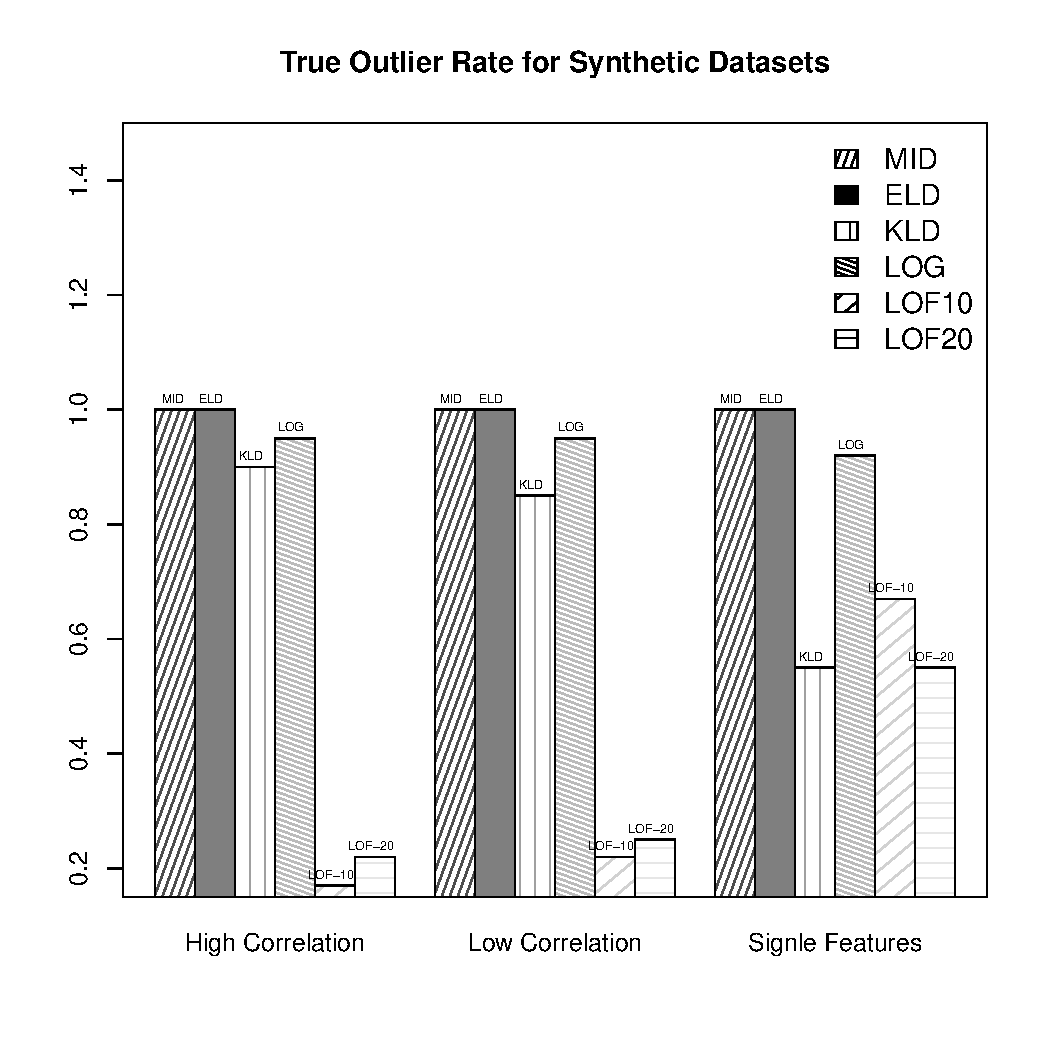
\includegraphics[height=70mm, width=70mm] {figures/TPR-Synthetic.pdf}
							%}
							%\subfigure{
							%  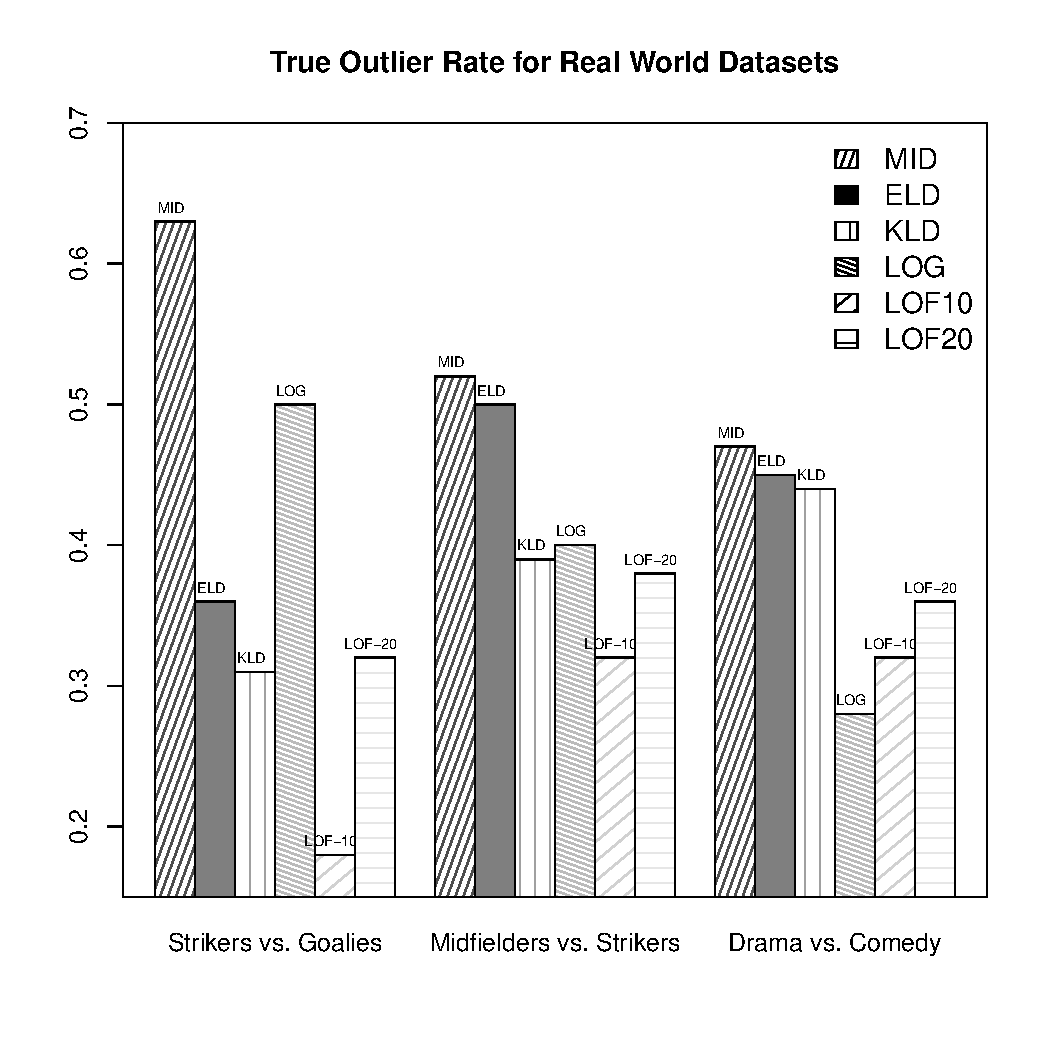
\includegraphics[height=70mm, width=70mm] {figures/TPR-All.pdf}
							
							% }
							% }
							
							%\caption{Comparison of Object Outlier Metrics}
							%\label{fig:synthetic}
							%\end{figure*}
							
							\subsection{Case Studies} \label{sec:CaseStudy} For a case study, we examine the three top outliers as ranked by $\mid$, shown in Table~\ref{table:CaseStudy}. 
							The aim of the case study is to provide a qualitative sense of the outliers indicated by the scores. Also, we illustrate how the BN representation leads to an interpretable ranking. 
							Specifically, we employ a {\em feature-wise decomposition} of the score combined with a {\em drill down} analysis: 
							
							\begin{enumerate}
								\item Find the node $\feature_{i}$ that has the highest $\mid_{i}$ divergence score for the outlier object. 
								\item Find the parent-child combination that contributes the most to the $\mid_{i}$ score for that node.
								\item Decompose the $\mid_{i}$ score for the parent-child combination into feature and mutual information component. 
							\end{enumerate}
							
							We present strong associations---indicated by the $\mid$'s mutual information component---in the intuitive format of association rules. Association analysis can also be applied to $\lr$ using the form~\eqref{eq:decompose}; we focus on $\mid$ for brevity.
							
							%\begin{figure}
							%\centering
							%   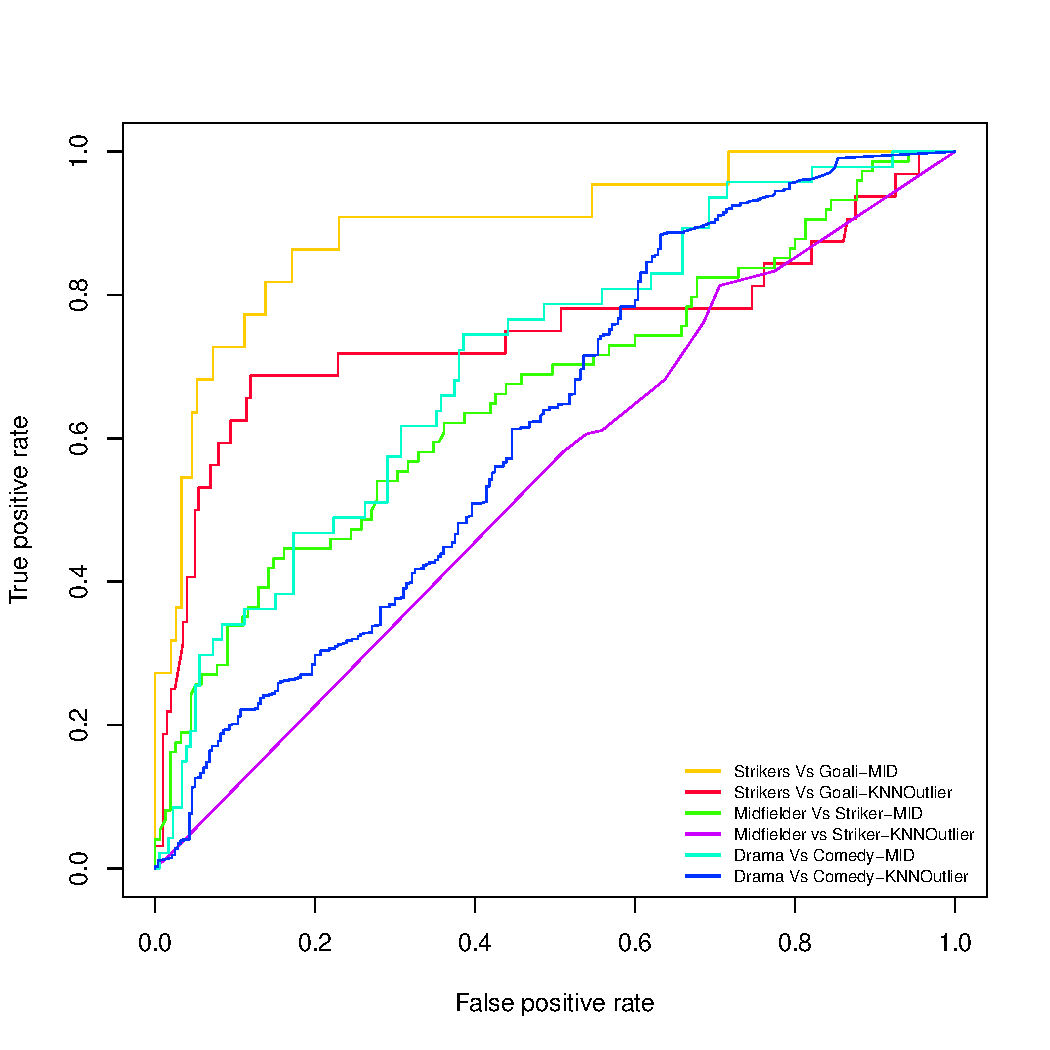
\includegraphics[width=1\textwidth] {figures/ROCKNN.pdf}
							% \caption{Detection Accuracy of $\mid$ vs. $\knn$
							% \label{fig:ROC}}
							%\end{figure}
							%\vspace{-5mm}
							\paragraph{Strikers vs. Goalies.} 
							%The Mutual Information Score $\mid$ separates goalies from Strikers better compared to the other methods.  
							%
%							In real-world data, a rare object may be a {\em in-class outlier}, i.e., highly anomalous even within its class. In an unsupervised setting without class labels, we do not expect an outlierness score to distinguish such an in-class outlier from outliers outside the class. 
							%								This is the reason why in real-world data, we do not expect an outlier detection score to distinguish the normal class objects perfectly from objects outside the class. 
							Edin Dzeko is  highly anomalous striker who obtains 
							the top $\mid$ outlierness score among both strikers and goalies. His $\mid$ score is highest for the Dribble Efficiency feature. The highest $\mid$ score for that feature occurs when Dribble Efficiency is low, and its parents have the following values: Shot Efficiency = high, Tackle Efficiency = medium. Looking at the single feature divergence, 
							%Decomposing this $\mid$ score into feature divergence and joint information divergence, 
							we see that Edin Dzeko is indeed an outlier in the Dribble Efficiency subspace: His dribble efficiency is low in 16\% of his matches, whereas a randomly selected striker has low dribble efficiency in 50\% of their matches. Thus, Edin Dzeko is an unusually good dribbler. Fans have recognized his skill by posting many examples of Dzeko dribbling on Youtube. Looking at the mutual information component of $\mid$, for Edin Dzeko the confidence of the rule 
							$$\it{ShotEff} = \it{high}, \it{TackleEff} = \it{medium}\rightarrow \it{DribbleEff} = \it{low}$$ is 50\%, whereas in the general striker class it is $38\%$. Therefore his Shot Efficiency and Tackle Efficiency have an unusually high association with his Dribble Efficiency.
							%The $\eld$ divergence also ranks Edin Dzeko as unusual. But because it allows feature and joint information divergence to cancel, his rank is somewhat lower. The likelihood metric does not recognize him as unusual at all. 
							
							%								The next two outliers according to $\mid$ are goalies Paul Robinson and Michel Vorm. Their rank is based only on feature divergence, with zero mutual information distinction. The maximum feature divergence is obtained by the $\it{SavesMade}$ feature. This makes intuitive sense since strikers basically never make saves. 
							%In other words, feature divergence with respect to $\it{SavesMade}$ is a good way to distinguish goalies from strikers. 
							%
							%The $\eld$ divergence also ranks Paul Robinson and Michel Vorm as clear goalies.  The likelihood metric does not recognize Paul Robinson as unusual at all. 
							%\vspace{-5mm}
							\paragraph{Soccer Midfielders vs. Strikers.} 
							%The  $\mid$ metric separates midfielders from strikers better compared than the other methods.  
							%The single feature divergence does not discriminate these two classes of objects. Intuitively, this is because strikers and midfielders are generally similar with respect to single features.  
							%The distance metrics have a better TOR rate than the averaging metrics. 
							
							%	The decomposition analysis for the top three $\mid$ outliers proceeds as follows. 
							For the single feature score, Robin van Persie is recognized as a clear striker because of the $\it{ShotsOnTarget}$ feature. It makes sense that strikers shoot on target more often than midfielders. Robin van Persie  achieves a high number of shots on targets in $34\%$ of his matches, compared to $3\%$ for a random midfielder. The mutual information component shows that he also exhibits  unusual correlations. For example, 
							the confidence of the rule
							$$\it{ShotEff} = \it{high}, \it{TimePlayed} = \it{high} \rightarrow \it{ShotsOnTarget} = \it{high}$$
							is 70\% for van Persie, whereas for strikers overall it is 52\%.
							%Both the $\eld$ metric and the $\lnlikelihood$ metric recognize Van Persie as a striker. 		
							%								Wayne Rooney is recognized as a striker for similar reasons, but less clearly because he achieves a high number of shots on target less frequently. 
							The most anomalous midfielder is Scott Sinclair. His most unusual feature is $\it{DribbleEfficiency}$: For feature divergence, he achieves a high dribble efficiency $50\%$ of the time, compared to a random midfielder with $30\%$. 
							%The $\jid$ divergence shows that he also exhibits unusual correlations for DribbleEfficiency.
							%The $\eld$ divergence too ranks Scott Sinclair as an unusual midfielder, whereas the likelihood method places him in the middle of his class. 
							%\vspace{-5mm}
							\paragraph{Drama vs. Comedy.} 
							%As with the other data sets, the  $\mid$ metric separates normal objects  from the contrast class better than the other methods.   
							The top $\mid$ rank is assigned to the in-class outlier $\it{Brave Heart}$. Its most  unusual feature is  $\it{ActorQuality}$: In a random drama movie,  $42\%$ of actors have the highest quality level 4, whereas for $\it{Brave Heart}$ $93\%$ of actors achieve the highest quality level. 
							%The $\eld$ divergence also ranks $\it{Brave Heart}$ as an unusual drama, whereas the likelihood method places it in the middle of its class. 		
							%based on user assigned ranking. 
							The  $\mid$ score identifies the comedies  $\it{Blues Brothers}$ and $\it{Austin Powers}$ as the top out-of-class outliers. 
							%	The main contributor to these rankings is the $\it{Cast\_Position}$ feature. 
							In a random drama movie,  $49\%$ of actors have casting position 3, whereas for $\it{Austin Powers}$ $78\%$ of actors have this casting position, and for $\it{Blues Brothers}$ $88\%$ of actors do. 
     						\paragraph{Hockey Defenders vs. Forwards.}
     						The first two players in the ranking are Forwards; the high outlierness ranking is mainly due to their unusually high value for points. Eric Staal has $\it{points=2}$ in 30\% of his matches, while a random player has that value for points only on 6\% of his matches. Dustin Byfuglien is an in-class outlier. His most unusual feature is $\it{Power Play Time}$. While an average player shows  $\it{Power Play Time=2}$ for only 33\% of his matches, Byfuglien's percentage is 79\%. 
%						

						
							%								These three movies also show unusual correlations for this feature with high divergence in the mutual information component (not shown in Table~\ref{table:CaseStudy}).
%							\begin{table*}
%								\centering
%								\caption{Case study for the top outliers returned by the log-likelihood distance score \mid
%									\label{table:CaseStudy}}
%								\resizebox{1\textwidth}{!}{
%									\begin{tabular}{|l|l|l|l|l|l|} \hline
%										\multicolumn{8}{|c|}{Strikers (Normal) vs. Goalies (Outlier)}\\
%										\hline
%										PlayerName&Position&$\mid$ Rank&$\mid$ Max Node&$\mid$ Node Score&$\fd$ Max feature Value \\ \hline
%										Edin Dzeko&Striker&1&DribbleEfficiency&83.84\\ \hline
%										Paul Robinson&Goalie&2&SavesMade&49.4&SM=Medium\\ \hline
%										Michel Vorm&Goalie&3&SavesMade&85.9&SM=Medium\\ \hline
%										\multicolumn{8}{|c|}{Midfielders (Normal) vs. Strikers (Outlier)}\\
%										\hline
%										PlayerName&Position&$\mid$ Rank&$\mid$ Max Node&$\mid$ Node Score&$\fd$ Max feature Value \\ \hline
%										Robin Van Persie& Striker&1&ShotsOnTarget&153.18&ST=high \\ \hline
%										Wayne Rooney& Striker&2&ShotsOnTarget&113.14&ST=high\\ \hline
%										Scott Sinclair&Midfielder&6&DribbleEfficiency&71.9&DE=high\\ \hline
%										\multicolumn{8}{|c|}{Drama (Normal) vs. Comedy (Outlier)}\\
%										\hline
%										MovieTitle&Genre&$\mid$ Rank&$\mid$ Max Node&$\mid$ Node Score& $\fd$ Max feature Value\\ \hline
%										Brave Heart&Drama&1&ActorQuality&89995.4&a\_quality=42\\ \hline
%										Austin Powers&Comedy&2&Cast\_Position&61021.28&Cast\_Num=3\\ \hline
%										Blue Brothers&Comedy&3&Cast\_Position&24432.21&Cast\_num=3\\ \hline
%									\end{tabular} 
%								}
%							\end{table*}

				\begin{table}
					\centering
				
					\resizebox{1\textwidth}{!}{
						\begin{tabular}{llllll} \hline
							\multicolumn{6}{|c|}{Strikers (Normal) vs. Goalies (Outlier)}\\
							\hline
							PlayerName&Position&$\mid$ Rank&$\mid$ Max Node&$\mid$ Node Score&$\fd$ Max feature Value \\ \hline
							Edin Dzeko&Striker&1&DribbleEfficiency&83.84&DE=low \\ \hline
							Paul Robinson&Goalie&2&SavesMade&49.4&SM=Medium4\\ \hline
							Michel Vorm&Goalie&3&SavesMade&85.9&SM=Medium\\ \hline
							\multicolumn{6}{|c|}{Midfielders (Normal) vs. Strikers (Outlier)}\\
							\hline
							PlayerName&Position&$\mid$ Rank&$\mid$ Max Node&$\mid$ Node Score&$\fd$ Max feature Value \\ \hline
							Robin Van Persie& Striker&1&ShotsOnTarget&153.18&ST=high \\ \hline
							Wayne Rooney& Striker&2&ShotsOnTarget&113.14&ST=high\\ \hline
							Scott Sinclair&Midfielder&6&DribbleEfficiency&71.9&DE=high\\ \hline
							\multicolumn{6}{|c|}{Drama (Normal) vs. Comedy (Outlier)}\\
							\hline
							MovieTitle&Genre&$\mid$ Rank&$\mid$ Max Node&$\mid$ Node Score& $\fd$ Max feature Value \\ \hline
							Brave Heart&Drama&1&ActorQuality&89995.4&a\_quality=4\\ \hline
							Austin Powers&Comedy&2&Cast\_Position&61021.28&Cast\_Num=3\\ \hline
							Blue Brothers&Comedy&3&Cast\_Position&24432.21&Cast\_num=3\\ \hline
								\multicolumn{6}{|c|}{Defender (Normal) vs. Forward (Outlier)}\\
								\hline
								PlayerName&Position&$\mid$ Rank&$\mid$ Max Node&$\mid$ Node Score& $\fd$ Max feature Value \\ \hline
								Eric Staal&Forward&1&Points&49.57&Points=2\\ \hline
								Phil Kessel&Forward&2&Points&43.34&Points=2\\ \hline
								Dustin Byfuglien&Defender&3&Power\_PlayTime&25.65&PP\_time=2\\ \hline
						\end{tabular} 
					}
						\caption{Case study for the top outliers returned by the  \mid score
							\label{table:CaseStudy}}
				\end{table}

\section{Correlation with Success}
\label{sec:success}

%OS: I put previous writing after \end{document}
%\subsection{Experiments}
%\subsubsection{Datasets}

The aim of this section is to compare the $\mid$ metric with other meaningful metrics for comparing individuals. Our reference metrics are {\em success rankings} of individuals selected for a specific domain, shown in Table~\ref{table:metrics}. We use the same data as in our other experiments, described in Section~\ref{sec:Experiments}. (We left out Mutagenesis as there is no meaningful success metrics for that data set.)

Success rankings are one of the most interesting features to users. Strong correlations between the $\mid$ metric and meaningful success metrics provide evidence that the $\mid$ metric is meaningful as well. We measure correlation strength by the standard Pearson correlation coefficient $\rho$. The coefficient ranges from -1 to 1, where 0 means no correlation and 1 or -1 indicates maximum strength~\citep{Fisher1921}.

The observed correlations are remarkable in at least two respects. 
\begin{enumerate}
\item The strength of the correlations are high. For example, between $\mid$ and salary, coefficients range from 0.45 to 0.82 (see Table~\ref{table:ELDwithPlayer}).
\item We observe high correlations across different domains, different types of individuals, and different success metrics. 
\end{enumerate}



\begin{table}[htbp]
	
	\centering
	\resizebox{1\textwidth}{!}{
		\begin{tabular}{llllll}
			\hline
			Dataset&Success Metric&Min&Max&Standard Dev.&Mean\\ \hline
			IMDb & Sum of Rating & 1.0 & 14795 & 1600.22 & 1057.58\\ \hline
			PL-Player &TimePlayed& 5.0 & 3420 & 1015.69 & 1484.00\\ \hline
			PL-Player&Normalized Salary&0.007&0.28&0.62&0.10\\\hline
			PL-Player&Sum of Shot Efficiency&0&82&9.87&6.53\\\hline
			PL-Team &Standing& 1.0 & 20 & 5.91 & 10.50\\ \hline

			NHL-Player&Power Play Time& 0 & 669 & 106.78 & 84.38\\ \hline			
			NHL-Player&Time on Ice& 4 & 2099 & 278.03 & 1187.31\\ \hline								NHL-Player&Assists& 0 & 4 & 0.49 & 0.20\\ \hline			
		\end{tabular}}
		\caption{Success metrics and their distributions.\label{table:metrics}}	
	\end{table}



For a population with a diverse set of skills and resources,
%apart from a serious decline in quality of generalization, 
being different from the generic class can be interpreted as both exceptionally better or worse than the normal population. In the domains we study in this data, we found that higher $\mid$ scores point to exceptionally good individuals but not to exceptionally bad individuals. Our interpretation of the correlation between $\mid$ and success, rather than failure, is that our domains featured skilled individuals, so a normal individual is quite successful already. 
For example, in the Premier League we expect most players to be in the range of good players. Therefore, deviating from the rest of the population is a signal for detecting exceptionally good players. Our $\mid$-success scatterplots below (Figure~\ref{fig:strikersELD}) provide empirical evidence for this interpretation: we typically see a large cluster of individuals around the origin, meaning that their success level is normal and their $\mid$ score is low. %\textcolor{red}{maybe refer to the specific plots}. 

\paragraph{Discussion of Success Metrics.}
Sum of ratings for movies and league standing for teams are immediate measures of success. Measures like time played and shot efficiency are proxies for success that are widely used in sports analytics. 
%While we believe these proxies suffice to validate our outlierness metrics, r
Recent work in sports analytics has introduced sophisticated new performance metrics with several advantages. For example, time played is sensitive to factors beyond a player's control, such as injuries and coaching tactics.  By contrast, the goal impact metric, which is based on reinforcement learning, focuses on the value of the individual actions a player performs \citep{Routley2015a,Liu2018}. 

Our outlierness metrics are computed from instantiation counts (e.g. total passes in a match). However, their definition does not entail that they are proportional to such counts, for two reasons: 
i) The metrics are normalized to frequencies (e.g. passes per match, not total passes over all matches). ii) The metrics measure not directly the frequencies, but the {\em difference in frequencies} between a random and a specific individual.  The correlation between our outlierness metrics and count-based success measures can therefore not be explained as a matter of definition only.




\subsection{Methodology}

We report the correlations between the $\mid$ metric and metrics of success for a specific domain. We also focus on some unusually successful individuals as case studies. 
In considering the correlation between $\mid$ and success, it is useful to investigate subgroups of individuals to ensure an apples-to-apples comparison~\citep{Sun2009}. For instance, the attributes that lead to success are different for strikers and goalies.  Accordingly, we report correlations for subgroups as well as entire classes of individuals. We found that compared to other model-based outlierness metrics, $\mid$ shows the strongest correlation with success for all metrics and subgroups, except for the log-likelihood metric; detailed comparisons follow in Section~\ref{sec:corr-others}. 
	
%	Another point to consider is that, in BN generalization, similar to statistical generalization, population size and the structure of the  individuals is important. For example, in the Premier League, when the goal is to predict the success of  teams, there is no strong correlation between the ELD metric and standing of the teams as we expected it to be similar to the other domain/individuals ($\rho(Standing, ELD)=-0.21$). This could be due to the diverse and yet very small population (20 teams in total). But when we decrease diversity by evaluation only top 10 teams in the Premier League standing, correlation becomes a lot more stronger ($\rho(Standing, ELD)=-0.71$).


\subsection{Correlations between the $\mid$ outlier metric and success}

The next three tables summarize the observed correlations between success and $\mid$ metrics: Teams in Table~\ref{table:teamELD}, Players in Table~\ref{table:ELDwithPlayer},  Movies in Table~\ref{table:ELDmovie}.
		
							\begin{table}
						
									\centering
									\resizebox{0.4\textwidth}{!}{
										\begin{tabular}{lc}
											\hline
											Team&Standing\\\hline
											Top Teams&-0.71\\\hline
											Bottom Teams&-0.33\\\hline
											All Teams&-0.13\\\hline
										\end{tabular}
									}			\caption{Correlation between $\mid$ metric and standing of Teams. The best standing is place 1. \label{table:teamELD}}
								\end{table}

				
				\begin{table}
		
					\centering
					\resizebox{1\textwidth}{!}{
						\begin{tabular}{lcccccc}
							\hline
					Class&Time Played&Salary&Saves Made&Shots On target&Pass Efficiency\\\hline
					Strikers&0.86&0.82&NA&0.79&NA\\\hline
					Midfielders&0.80&0.45&NA&NA&0.77\\\hline
					Goalies&0.77&NA&0.74&NA&NA\\\hline
					All players&0.18&0.56&NA&NA&NA\\\hline
							%Synthetic&40&280\\ \hline
						\end{tabular}}
									\caption{Correlation between $\mid$ metric and success metrics of Soccer Players.}
									\label{table:ELDwithPlayer}
					\end{table}

								
								

%\begin{table}[htbp]
%	\caption{Correlation between $\mid$ metric and success metric of Goalies . \textbf{make single table. Probably make the rows the metrics, the columns the classes, including the whole population. Or add a row for all players. See our aaa2014.tex paper. } \label{table:players}}
%	\centering
%	\resizebox{0.7\textwidth}{!}{
%		\begin{tabular}{|c|c|c|c|}
%			\hline
%			Metric&Sum of SavesMade&TimePlayed&Salary\\\hline
%			$\mid$&0.71&0.73&0.6\\\hline
%		\end{tabular}}
%		\caption{Correlation between $\mid$ metric and success metric of Midfielders. \label{table:Midfielders}}
%		\resizebox{1\textwidth}{!}{
%			\begin{tabular}{|c|c|c|c|c|}
%				\hline
%		Metric&Sum of Pass Efficiency&Sum of dribble Efficiency&TimePlayed&Salary\\\hline
%		$\mid$&0.89&0.76&0.80&0.45\\\hline
%			\end{tabular}
%			
%			}
%				\caption{Correlation between $\mid$ metric and success metric of Strikers .\label{table:strikers}}
%					\resizebox{0.7\textwidth}{!}{
%						\begin{tabular}{|c|c|c|c|}
%							\hline
%							Metric&Shots On Target&TimePlayed& Salary\\\hline
%							$\mid$&0.72&0.82&0.79\\\hline
%						\end{tabular}
%						
%					}
%\caption{Correlation between $\mid$ metric and success metric of Movies .\label{table:movie}}
%\resizebox{0.8\textwidth}{!}{
%	\begin{tabular}{|c|c|c|c|}
%		\hline
%	Genre&Sum of Rating&Average of Rating&Number of Rating\\\hline
%	Action&0.68&0.30&0.72\\\hline
%	Drama&0.78&0.29&0.81\\\hline
%	Comedy&0.85&0.41&0.84\\\hline
%	All Movies&0.56&0.17&0.60\\\hline
%		\end{tabular}
%}
%		\end{table}
%		
%
		
		\begin{table}

			\centering
		\resizebox{0.8\textwidth}{!}{
			\begin{tabular}{lccc}
				\hline
				Genre&Sum of Rating&Average of Rating&Number of Rating\\\hline
				Action&0.67&0.30&0.72\\\hline
				Drama&0.76&0.29&0.81\\\hline
				Comedy&0.85&0.41&0.84\\\hline
				All Movies&0.56&0.17&0.60\\\hline
			\end{tabular}
		}		\caption{Correlation between $\mid$ metric and success metric of Movies.\label{table:ELDmovie}}
	\end{table}
	
	
	

			
\subsubsection{Soccer Teams} 
\paragraph{Team Standing.}
	The most successful team has Standing=1 and the least successful team has Standing=20 in the 2011-2012 Season. Figure~\ref{fig:TeamStandingELD} shows the correlation of $\mid$ with team success metrics in a scatter plot. For the top teams, a very strong negative correlation emerges between $\mid$ and standing: teams with higher $\mid$ achieve a better (lower) standing. 
	 The top two teams Manchester City and Manchester United stand out very strongly in terms of the $\mid$ metric (bottom right corner).

\begin{figure}[t]
	\centering
	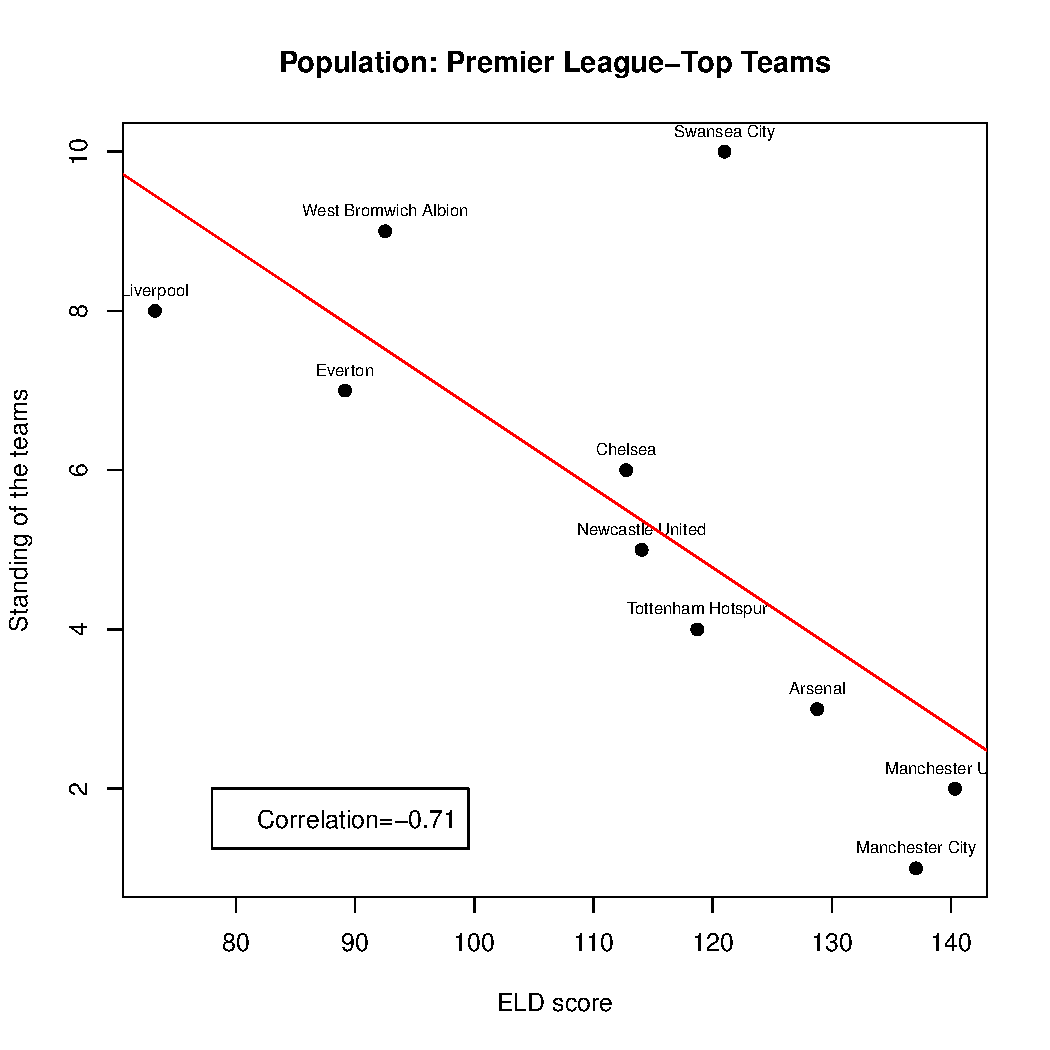
\includegraphics[width=0.8\textwidth]{topTeamStats-Sep.pdf}
	
	\caption{Teams: Team Standing vs. $\mid$ for the top teams in Premier League. 
		\label{fig:TeamStandingELD}}
\end{figure}

\subsubsection{Soccer Players}

	\paragraph{Players Time Played} is the total time that a player played over all matches in the season. This metric was shown to correlate strongly with other success metrics, such as salary, in soccer data~\citep{schwartz}. 
%	Tables ~\ref{table:goalie} and \ref{table:players} 
%	
%	and Figures \ref{fig:GoalieTime} and \ref{fig:StrikerTime} 
%	
%	show the correlation between the ELD metric and time played. 
	For each subgroup, there is a strong positive correlation with $\mid$, meaning that atypical players with higher $\mid$ tend to play more minutes.
	
	%The results are mixed; they show that pay cannot be adequately explained by past performance
%	alone, nor are pay levels justified by future performance. The bids for players in the initial
%	auction appear to have been based on intangibles that are hard to quantify%
	\paragraph{Salary} is probably the most obvious, and at the same time often the most misleading way to measure success of the players. Previous studies suggest that salary of the players does not  always follow their performance in many sports such as Baseball and Soccer~\citep{Hall2002,Barrio2004}. They show that pay cannot be explained only by past performance but also depends on other factors that are hard to quantify. 
	
	 We manually collected salaries of 120 players from internet sources. Table \ref{table:ELDwithPlayer}  and Figures~\ref{fig:strikersELD} and \ref{fig:goaliesELD} show the correlation between $\mid$ and this success metric. The correlation is high, especially for Strikers. We found salary data for only 5 goalies. We discuss the relatively weaker salary correlation for midfielders in more detail below.
	 
	 \paragraph{Shots on Target} applies to strikers only. This is defined as any shot attempt that would or does enter the goal if left unblocked. We record the total number of these shots over all matches of the strikers only. This metric was shown to correlate strongly with $\mid$ (see Table \ref{table:ELDwithPlayer}, Figure~\ref{fig:StrikerShot}).
	 %
	 Figure~\ref{fig:strikersELD} plots $\mid$ against striker success metrics summed over the entire 2011-2012 season. We observe a large cluster around the origin, which represents a large base of normal strikers with average salaries and low $\mid$ scores. The striker with the greatest $\mid$ score is Robin van Persie. He stands out in terms of Shots on Target, Time Played, and Salary. 
	 
	 %should probably label the points with individual names


	\begin{figure}
		\centering     %%% not \center
		\subfigure[Strikers: Salary vs $\mid$. ]{\label{fig:StrikerSalary}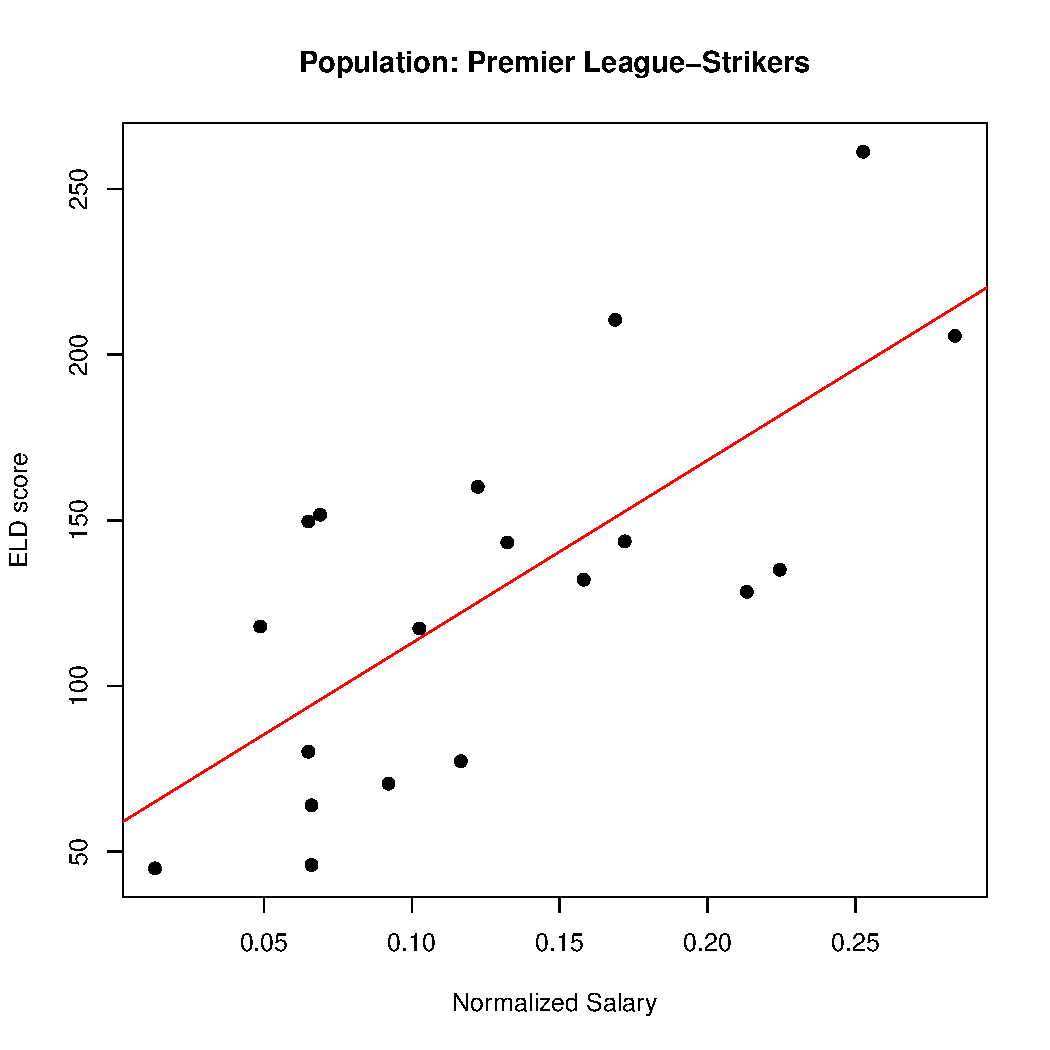
\includegraphics[width=0.65\textwidth]{1d-sumStrikerSalary.pdf}}
		\subfigure[Strikers: Shots On Target vs $\mid$]{\label{fig:StrikerShot}\includegraphics[width=0.65\textwidth]{1d-ShotsonTarget-sumStrikerStatistics.pdf}}
		\subfigure[Strikers: Time played vs $\mid$.]{\label{fig:StrikerTime}\includegraphics[width=0.65\textwidth]{1d-sumStrikerStatistics.pdf}}
		\caption{Correlations between $\mid$ and success metrics for strikers\label{fig:strikersELD}.}
	\end{figure}


	 
	\paragraph{Saves Made} applies to Goalies only. It is defined as the total number of saves that goalies had made over all the matches. This metric shows a strong correlation with $\mid$ as well (see Table~\ref{table:ELDwithPlayer}, Figure~\ref{fig:GoalieSaves}).  
	%
	Figure~\ref{fig:goaliesELD} shows a scatter plot with the correlation of $\mid$ with Goalie success metrics, summed over the entire 2011-2012 season. Goalies do not vary much in terms of the time they play. Wayne Hennessey has the highest number of Saves Made and also an unusually high $\mid$ score, although not the highest. 


	
	\begin{figure}
		\centering     %%% not \center
		\subfigure[Goalies: sum of time played vs $\mid$. ]{\label{fig:GoalieTime}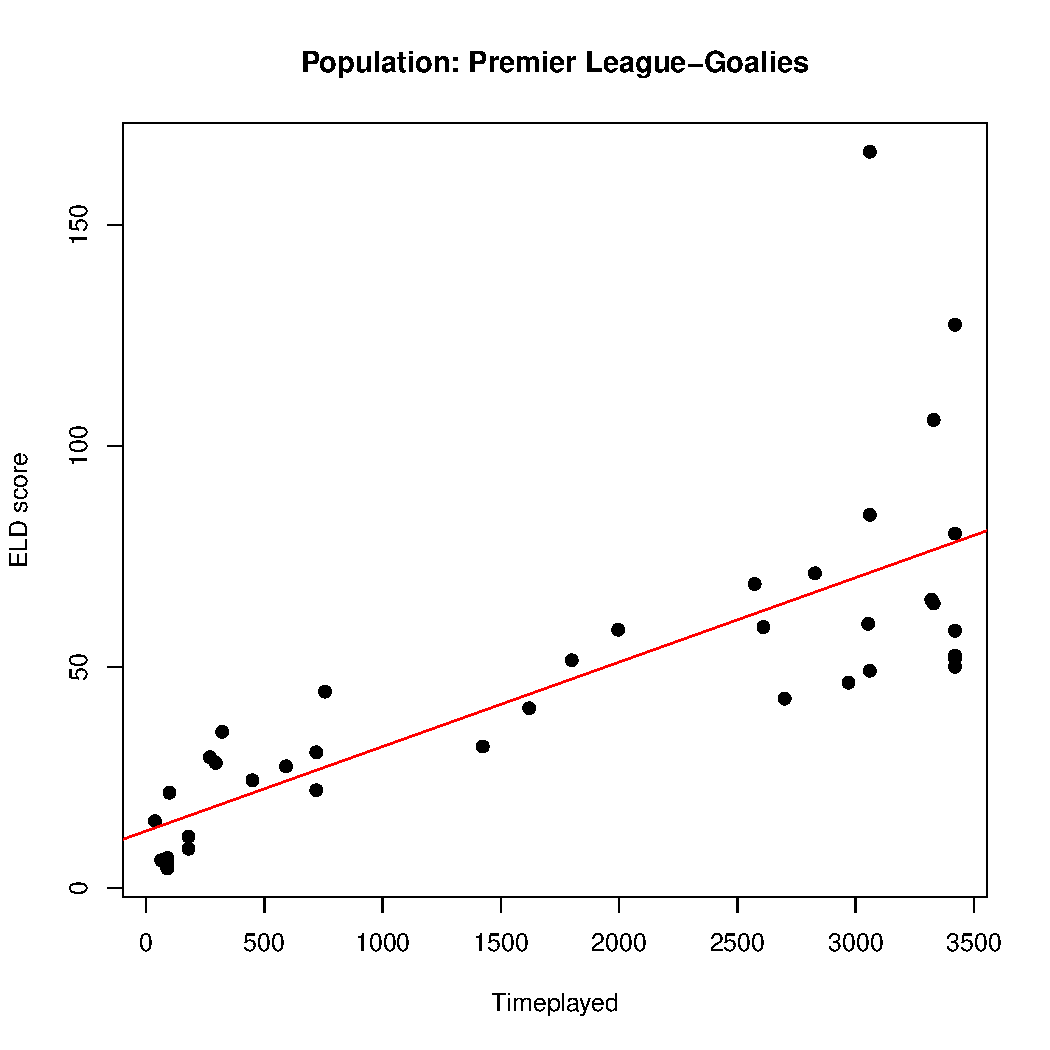
\includegraphics[width=0.7\textwidth]{sumGoalieStatistics.pdf}}
		\subfigure[Goalies: sum of saves made vs $\mid$]{\label{fig:GoalieSaves}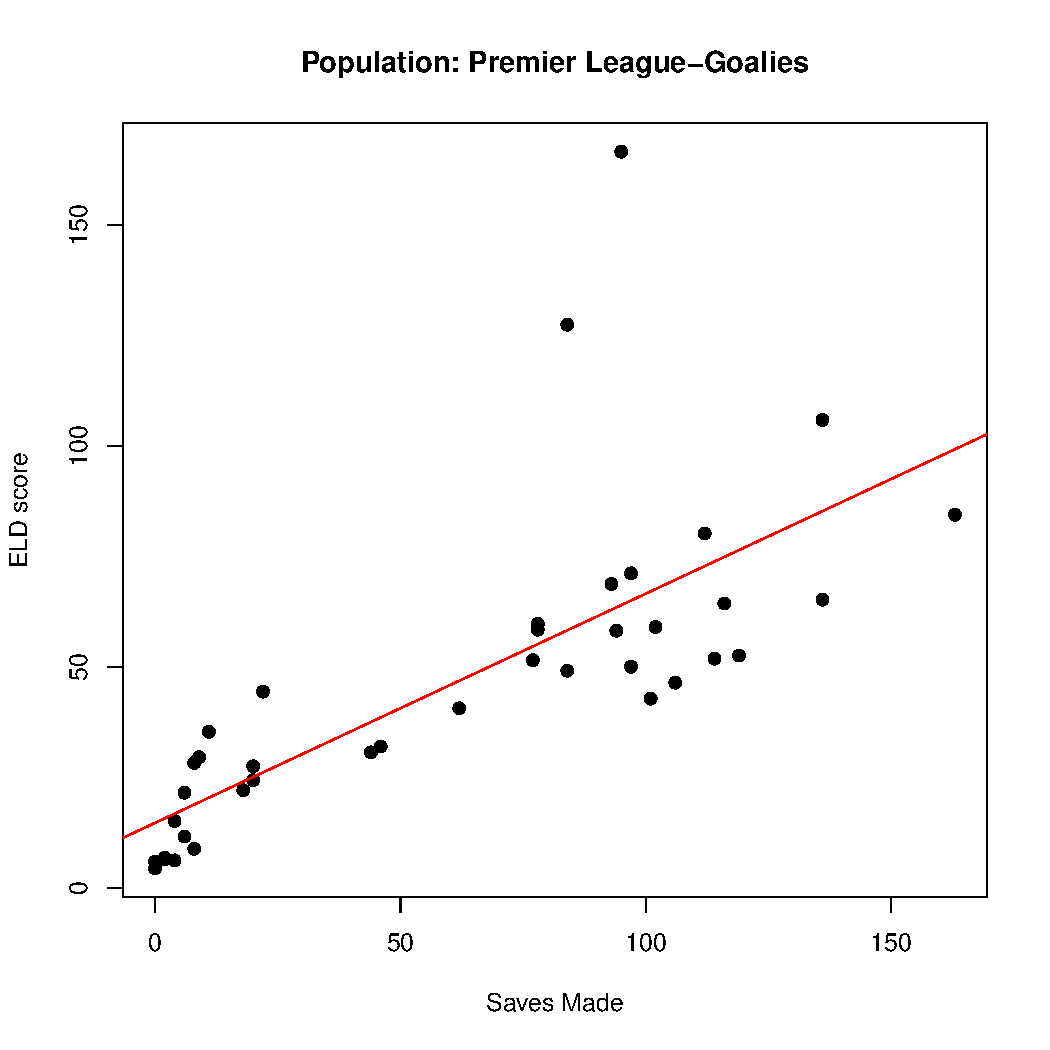
\includegraphics[width=0.7\textwidth]{sumGoalieStatisticsSavesMade.pdf}}
	%	\subfigure[Teams: Team Standing vs. $\mid$ for the top teams in Premier League. \textbf{separate figure please}]{\label{fig:TeamStanding}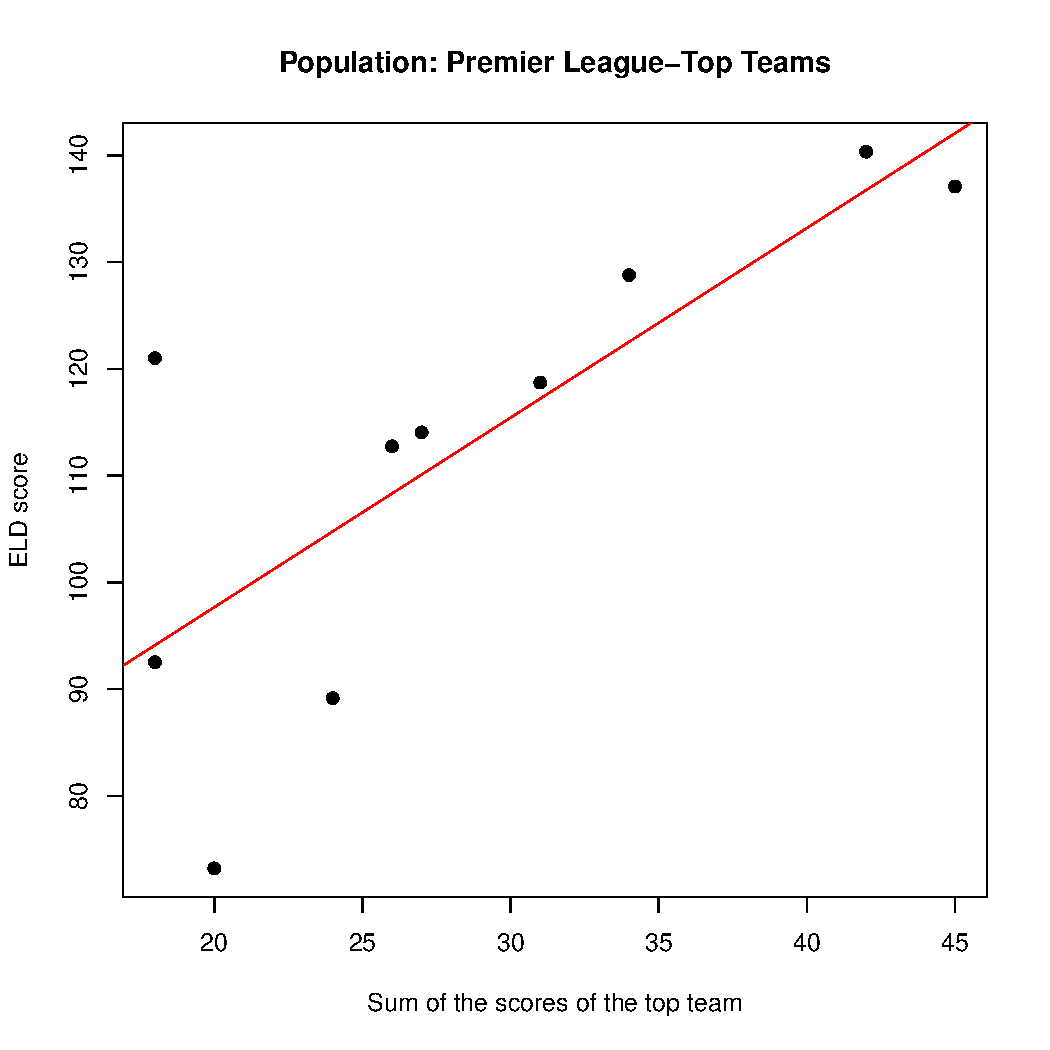
\includegraphics[width=0.5\textwidth]{topTeamStats.pdf}}
		\caption{Correlations between $\mid$ and success metrics for Goalies \label{fig:goaliesELD}}
	\end{figure}


\paragraph{Midfielder Salary.} We examine midfielder salaries for the 2011-2012 season.
We omit a scatterplot for midfielder salary vs. $\mid$ because it is less informative due to the weaker  correlation (0.45).
%
%While there is a strong correlation between salary of the Strikers and ELD score (0.79), this correlation becomes weaker in the Goalie population and even less apparent in Midfielder group. 
To investigate the reason for the weaker correlation, we picked two midfielders: 1) Stephane Sessegnon  who has been ranked second in the $\mid$ ranking but does not draw a large salary.  2) Steven Gerrard who is a very well known player and ranked second in the Salary ranking but according to the $\mid$ score, he has been ranked 21. Based on domain knowledge, we picked some of the features that are relevant to midfield performance from the raw data and compared the feature statistics for these two players. Table~\ref{table:MidfielderComparison} shows the details of their appearances in different matches. Sessegnon scored higher than Gerrard in three out of the four categories (Passes and Time Played). However, his salary was much lower than Gerrard's. Indeed his next contract with West Bromwich Albion netted him a club record fee. This is an example of how our $\mid$ metric can identify players who are underpaid relative to their potential.
%This is an example of how weak the correlation is between salary and the observed box scores, which are the basis for the $\mid$ metric. 
%to show how unfair and unreliable the salary is in this domain.
%	 Unsuccessful Passes&Successful Long Passes
		\begin{table}[htbp]
			
			\centering
			\resizebox{1\textwidth}{!}{
				\begin{tabular}{llccccccc}
					\hline
					Name&Team&age&\begin{tabular}{c}Salary\\Ranking \end{tabular}&\begin{tabular}{c}$\mid$\\Ranking \end{tabular}&\begin{tabular}{c}Time\\Played \end{tabular}&\begin{tabular}{c}Unsuccessful\\Passes \end{tabular}&\begin{tabular}{c}Successful\\Long Passes \end{tabular}&\begin{tabular}{c}Successful\\corners \end{tabular}\\\hline
					Steven Gerrard	&Liverpool&31&2&21&1212 min&244&52&25\\\hline
					Stephane Sessegnon&Sunderland&26&22&2&3133 min&231&82&15\\\hline
					
					%	$\mid$&0.71&0.73&0.6\\\hline
				\end{tabular}}
				%
				\caption{Comparison of two midfielders.\label{table:MidfielderComparison}}
			\end{table}

	
	
						
						\begin{table}
						
						
							\centering
							\resizebox{1\textwidth}{!}{
								\begin{tabular}{cccccc}
									\hline
									Class&Time On Ice &Power Play Time&Assists&Goals\\\hline
									Forwarder&0.79&0.78&0.81&0.78\\\hline
									Defender&0.66&0.57&0.60&0.40\\\hline
									
									%Synthetic&40&280\\ \hline
								\end{tabular}}
									\caption{Correlation between $\mid$ metric and success metrics of NHL Players.	\label{table:ELDwithHockey}}
							\end{table}
	\subsubsection{Hockey Players}
	For the hockey players the features that we have selected as success metrics are as follows: $\it{Time on Ice}$ is the total amount of time a player has played over the course of a season. $\it{Power Play Time}$ is the total amount of power player time for a player in a season. $\it{Assists}$ is the total number of any actions by a player that led to a goal. Finally we use the total number of $\it{Goals}$ that a player has scored.
The correlation between these features and $\mid$ is shown in Table~\ref{table:ELDwithHockey}. ELD has high correlations in features of both categories, however, it is stronger in the Forward subgroup.
	\subsubsection{Movies} 
	
	\paragraph{Movie Sum of Ratings} is the number of user ratings of a movie. Table~\ref{table:ELDmovie} shows a high correlation with the $\mid$ metric. The highest correlation obtains for the genre Comedy (0.84). 
	%See Figure~\ref{fig:ActionRate},Figure~\ref{fig:ComedyRate}, Figure~\ref{fig:DramaRate}). 
	The correlation between a movie and the sum of its ratings is equally strong, but the correlation with its average rating is much weaker. Thus the $\mid$ score is associated with how many users have rated the movie rather than with how they have rated it. The number of ratings is a meaningful success metric, as it measures the number of people who have gone to see the movie.  
	

%\textcolor{red}{need to fix cross-reference} Figure~\ref{fig:Movies} shows the correlation of $\mid$ with movie success metrics in a scatter plot. We again observe a large cluster of movies around the origin. For drama and comedy movies, the top rated movies are (``American Beauty'' resp. ``Being John Malkovich''); these also stand out in the $\mid$ metric. 


%	\begin{figure}
%		\centering     %%% not \center
%		\subfigure[Action movies: sum of ratings by users vs $\mid$. ]{\label{fig:ActionRate}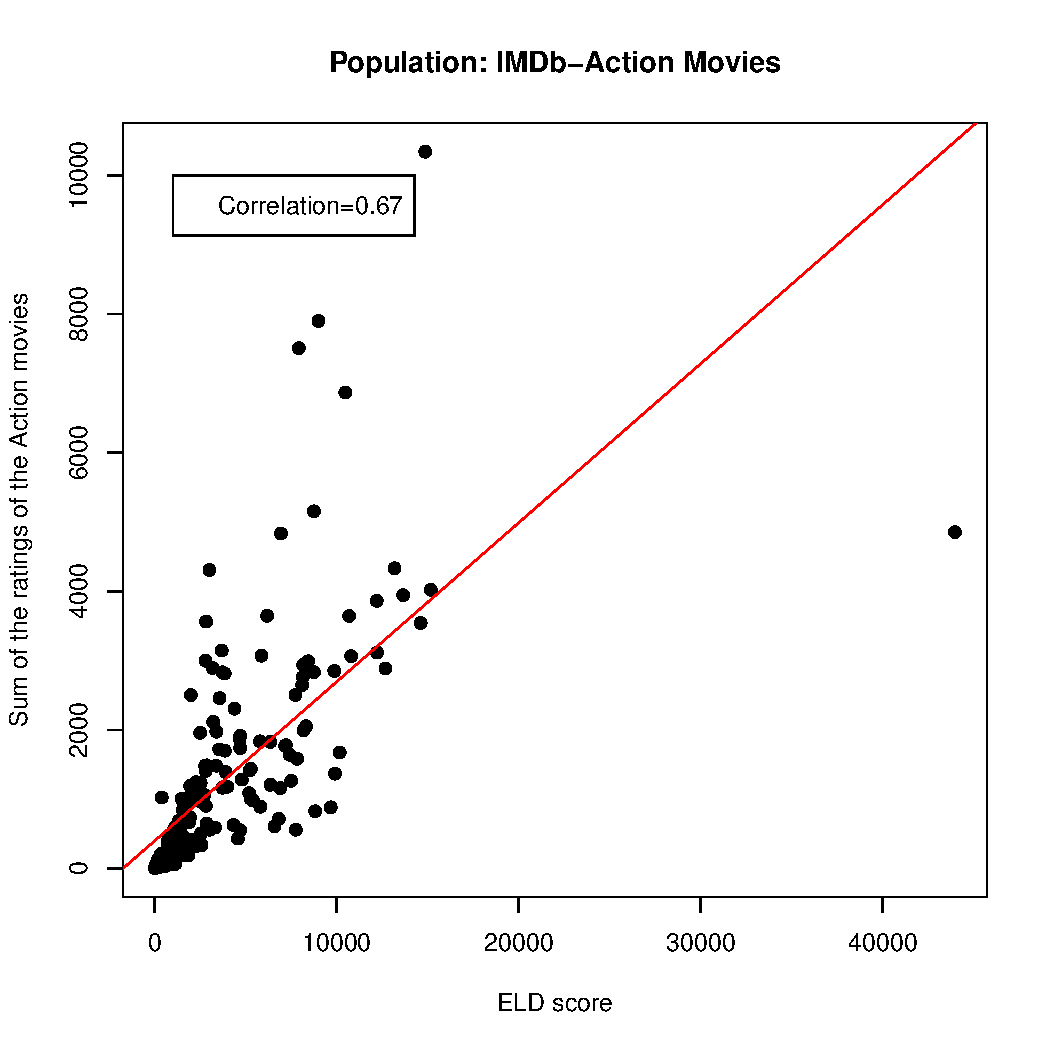
\includegraphics[width=0.48\textwidth]{NewPlotsJan2016/Action-Correlation.pdf}}
%		\subfigure[Comedy movies: sum of ratings by users vs $\mid$]{\label{fig:ComedyRate}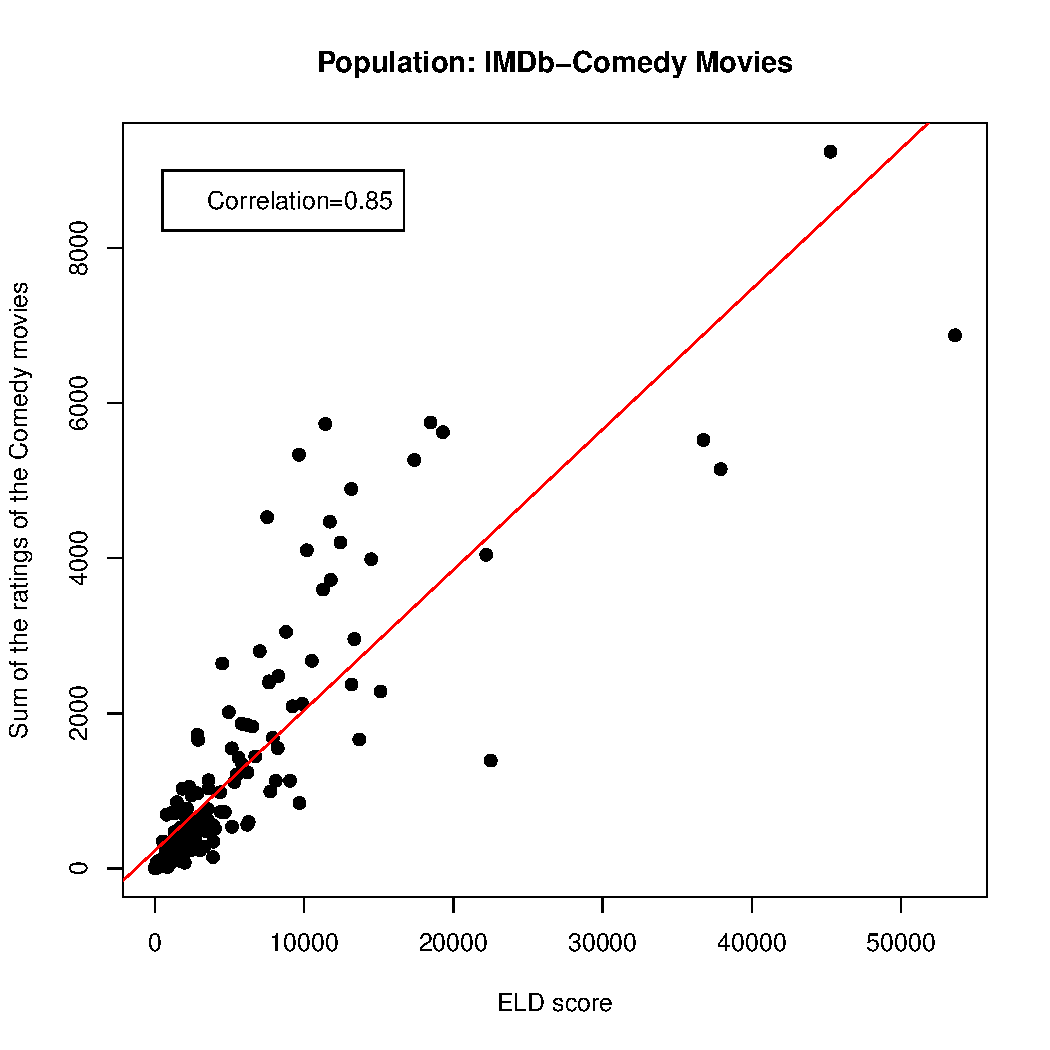
\includegraphics[width=0.5\textwidth]{NewPlotsJan2016/Comedy-Correlation.pdf}}
%		\subfigure[Drama movies: sum of ratings by users vs $\mid$.]{\label{fig:DramaRate}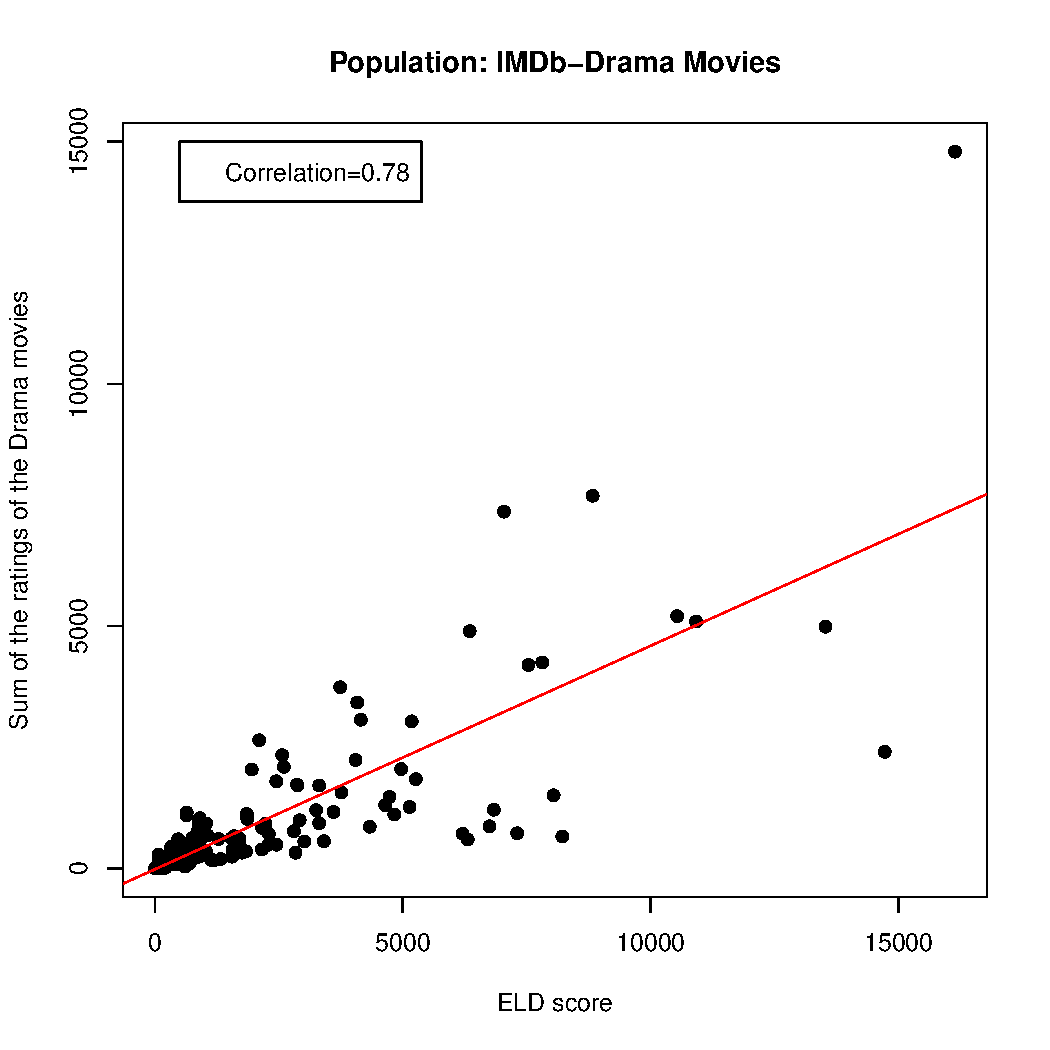
\includegraphics[width=0.5\textwidth]{NewPlotsJan2016/Drama-Correlation.pdf}}
%		\caption{\label{fig:Movies}}
%	\end{figure}


\subsection{Correlations between other outlierness metrics and success} \label{sec:corr-others}
In Section~\ref{sec:log} and~\ref{sec:metrics} we introduced other metrics that could be used in order to detect outliers. In this section we discuss the correlation between those metrics and success. The correlation between $\mid$ and success is always stronger than $\textit{FD}$ and $\textit{LR}$ in all the data sets and subgroups, therefore we omit those results. The Log-likelihood is the only metric that results in a stronger correlation in some data sets and subgroups. Table~\ref{table:correlationLOGELD} shows the subgroups for which log-likelihood shows a stronger correlation than the $\mid$ metric. 
A high correlation with success can be interpreted as detecting in-class outliers. This results shows that log-likelihood could be an alternative score for finding in-class outliers.
		\begin{table}

			\centering
			\resizebox{1\textwidth}{!}{
				\begin{tabular}{llcc}
					\hline
					Subgroup&Success metric&$\mid$ correlation&Log-likelihood correlation\\\hline
					Comedy&Sum of Rating&0.85&0.87\\\hline
					Drama&Sum of Rating&0.78&0.82\\\hline
					PL-Midfielder&Pass Efficiency&0.77&0.89\\\hline
					PL-Midfielder&Time Played&0.80&0.86\\\hline
					PL-Goalies&Time Played&0.77&0.87\\\hline
					PL-Goalies&Saves Made&0.74&0.85\\\hline
					NHL-Forward&Time on Ice&0.79&0.95\\\hline
					NHL-Forward&Goals&0.78&0.83\\\hline
		
					
				\end{tabular}
			}			\caption{Subgroups and success metrics for which the log-likelihood metric's correlates with success stronger than $\mid$.\label{table:correlationLOGELD}}
		\end{table}
		

\section{Limitation of Model-based outlier detection} 

Quantitative evaluation, case studies, and correlation with meaningful success metrics confirm the effectiveness of exceptional model mining as an outlier detection method for relational data. The main {\em limitations of our approach} are the following.



\begin{enumerate}
	\item Our proposed method ranks potential outliers, but does not set a threshold for a binary identification of outlier vs. non-outlier.
		\item Our current Bayesian network learning method can only be applied to discrete data. Prior to learning the model, we converted continuous data into discrete, which causes some information loss. 
		\item Our generative model-based methods learn a generic Bayesian network structure for the entire population, so the detected outliers are global outliers. However, there are  more complex outliers that locally deviate from their subgroups and can be detected only by subgroup comparison. One direction for future work is to first detect subgroups in the population and then outliers within subgroups.\footnote{We are indebted to Daniel Lowd for this point.}
		%		 \item In our 
	\end{enumerate}
	
Another limitation of our work is that, we used only part of the full information available in our rich data sets. Model-based outlier detection can be extended to take advantage of the full information, in the following manner. 
	\begin{enumerate}
		\item In the Premier League data set, players are naturally related to one another and modeling the interaction between players can be another way to detect anomalous players.
		Graph-based features, such as detecting near-clique nodes and star nodes, proved to be informative for anomaly detection as shown in the ODDBALL system~\citep{Akoglu2010}.
		\item In this paper we did not use the temporal information available in the data. In the learning process we do not give a higher weight to more recent observations. This point is especially important when applying the methods to dynamic data or the data that are collected over long periods of time. 
		\item We did not incorporate ways to estimate missing values in model learning and/or outlierness scores. 
%		However, real-world data sets may involve arbitrary pattens of missing data. Maximum likelihood density estimation is a way to estimate such values. 
		%We leave this feature for future work.
		%cite boosting in the presence of boosted statistical relational learning
		%WWe integrated out the individuals that had less than our specified threshold in the data. For example in the soccer domain, we did not include players who played less than five matches in our experiments. H 
	\end{enumerate}
		


\section{Conclusion and Future Work} We presented a new approach for applying Bayesian networks to object-relational outlier detection, a challenging and practically important topic for machine learning. The key idea is to apply the exceptional model mining framework as follows. First, use statistical-relational learning to construct from relational data a graphical model. Then learn one set of parameter values that represent class-level associations, another set to represent object-level associations, and compare how well each parametrization fits the relational data that characterize the target object. The classic metric for comparing two parametrized models is their likelihood ratio. As an novel alternative, we  define  a new relational outlierness score via two transformations:  (1) a mutual information decomposition, and (2) replacing log-likelihood differences by log-likelihood distances. This score combines a single feature component, where features are treated as independent, with a correlation component that measures the deviation in the features' mutual information.

In experiments on three synthetic and four real-world outlier sets, the EMM methods based on log-likelihood difference and the log-likelihood distance achieved the best detection accuracy. On all but one real-world data set, log-likelihood distance outperformed the log-likelihood difference. As an alternative to model-based EMM, converting the structured data to a flat data matrix via aggregation had a negative impact on outlier detection. 
Case studies showed that the EMM scores lead to easily interpreted rankings. We found that the expected log-likelihood distance score correlated with success metrics to a surprising degree, across different domains and classes of individuals. The correlation with metrics of independent interest corroborates that this outlierness score produces meaningful and interesting results.
%
%Overall, our new log-likelihood distance metric provides a promising new approach for applying machine learning techniques to outlier detection for object-relational data, a challenging and practically important topic. 

 							
There are several avenues for future work.  (i) A limitation of our current approach is that it ranks potential outliers, but does not set a threshold for a binary identification of outlier vs. non-outlier. (ii) Our divergence uses expected L1-distance for interpretability, but other metrics like L2 could be investigated as well. (iii) Extending the expected L1-distance for continuous features is a useful addition. (iv) Comparing our metric with the interestingness measures that have been developed for relational exception mining would increase our understanding of different how individuals can be unusual in structured data. (v) In the movie and soccer domains, our metric identified exceptionally successful individual objects, but not exceptionally unsuccessful ones. Our hypothesis was that in these domains, individuals have gone through a rigorous selection process, so the normal baseline performance is high. While we provided evidence for this hypothesis, it can be further investigated,  by applying our outlier detection to data sets that feature a range of skills, including both amateur and professional performance. (vi) The theoretical properties of our $\mid$ metric are important to understand. For example, when is the Taylor series approximation of $\mid$ by Total Variation Distance sufficient close that theoretical guarantees for TVD hold also for $\mid$?
%, and may facilitate combining our object-oriented approach with dimensional hierarchies in an OLAP data cube.
								%Distribution distances other than KLD could be evaluated for outlier detection (e.g., variation distance). However, the KLD variants have special advantages: their asymetry reflects the asymetry between object and class. Also, in a Bayesian network representation of the joint distributions, they decompose into a node-wise sum for easy computation and interpretation. 
								%A promising project for future work would be to combine the object data model and the multi-dimensional model to combine our object outlier method with OLAP-based methods. For example, one could add numeric measures and aggregate attributes to the object model. Another view: convert the object-oriented data to OLAP data, then use their outlier detection.
								
								
In sum, outlier metrics based on model likelihoods are a new type of structured outlierness score for object-relational data.  Our evaluation indicates that  model-based scores provide informative, interpretable, and accurate rankings of objects as potential outliers. 
								
\section*{Acknowledgements} This work was supported by a Discovery Grant from the Natural Sciences and Engineering Research Council of Canada. We are indebted for helpful discussions to the participants at the 2018 Workshop on Statistical Relational AI. The action editor and reviewers for the Data Mining and Knowledge Discovery Journal provided extensive helpful comments. We thank Peter Flach for clarifying the connection with exceptional model mining.

\section*{Appendix: Proofs} \label{sec:proofs}

We prove the results about $f$-divergences from Section~\ref{sec:theory}. We first review the known result that twice differentiable $f$-divergences are approximately scaled $\chi^{2}$-divergences. Second we prove our new result that our new $\mid$ metric is approximately total variation distance (plus a quadratic term with small impact).  

%For the ELD generator $f=-ln(u)$, we have $f'(1)=1$, so the first-order approximation to ELD is exactly TVD. 

{\em 
Assume that the generator $f$ is twice differentiable for $f$-divergence $I_{f}$. Then $I_{f}(P_{1}||P_{2}) \approx \frac{f''(1)}{2} \chi^{2}(P_{1}||P_{2}) = \frac{f''(1)}{2} 
\sum_{i=1}^{m}  \frac{(P_{2}(\nodevalue_{i})-P_{1}(\nodevalue_{i}))^{2}}
 {P_{1}(\nodevalue_{i})}$. 
}
\begin{proof}

Truncating the Taylor series for $f$ at $i=2$, the $f$-divergence expression~\ref{eq:f-divergence} becomes 

\begin{eqnarray*}
& & \sum_{i=1}^{m} P_{1}(\nodevalue_{i}) [f'(1) \left(\frac{P_{2}(\nodevalue_{i})}{P_{1}(\nodevalue_{i})}-1\right) + \frac{f''(1)}{2} \left(\frac{P_{2}(\nodevalue_{i})}{P_{1}(\nodevalue_{i})}-1\right)^{2}]  \\
& = &\sum_{i=1}^{m} P_{1}(\nodevalue_{i}) [f'(1) \left(\frac{P_{2}(\nodevalue_{i})-P_{1}(\nodevalue_{i})}{P_{1}(\nodevalue_{i})}\right) + \frac{f''(1)}{2} \left(\frac{P_{2}(\nodevalue_{i})-P_{1}(\nodevalue_{i})}{P_{1}(\nodevalue_{i})}\right)^{2}] \\
 & = & f'(1) [\sum_{i=1}^{m} P_{2}(\nodevalue_{i}) - \sum_{i=1}^{m} P_{1}(\nodevalue_{i})] + \sum_{i=1}^{m} \frac{f''(1)}{2} 
 \frac{(P_{2}(\nodevalue_{i})-P_{1}(\nodevalue_{i}))^{2}}
 {P_{1}(\nodevalue_{i})} \\
& = &   0 + \frac{f''(1)}{2} \chi^{2}(P_{1}||P_{2})
\end{eqnarray*}

\end{proof}

{\em The first-order Taylor series approximation for $\mid$ is total variation distance:
$$\mid(P_{1}||P_{2}) \approx  \TVD. $$}

\begin{proof}
Truncating the Taylor series for $f=-\ln(u)$ at $i=1$, the $|f|$-divergence expression~\ref{eq:f-absolute} becomes 

\begin{eqnarray}
& & \sum_{i:f(\frac{P_{2}(\nodevalue_{i})}{P_{1}(\nodevalue_{i})})>0} P_{1}(\nodevalue_{i}) f'(1) \left(\frac{P_{2}(\nodevalue_{i})}{P_{1}(\nodevalue_{i})}-1\right) -  \sum_{i:f(\frac{P_{2}(\nodevalue_{i})}{P_{1}(\nodevalue_{i})})<0} P_{1}(\nodevalue_{i}) f'(1) \left(\frac{P_{2}(\nodevalue_{i})}{P_{1}(\nodevalue_{i})}-1\right) \notag \\
& = &\sum_{i:f(\frac{P_{2}(\nodevalue_{i})}{P_{1}(\nodevalue_{i})})>0} P_{1}(\nodevalue_{i}) f'(1) \left(\frac{P_{2}(\nodevalue_{i})-P_{1}(\nodevalue_{i})}{P_{1}(\nodevalue_{i})}\right) - \sum_{i:f(\frac{P_{2}(\nodevalue_{i})}{P_{1}(\nodevalue_{i})})<0} P_{1}(\nodevalue_{i}) f'(1) \left(\frac{P_{2}(\nodevalue_{i})-P_{1}(\nodevalue_{i})}{P_{1}(\nodevalue_{i})}\right) \notag \\
 & = & 
- \sum_{i:P_{2}(\nodevalue_{i})<P_{1}(\nodevalue_{i})}
P_{2}(\nodevalue_{i})-P_{1}(\nodevalue_{i}) + \sum_{i:P_{2}(\nodevalue_{i})>P_{1}(\nodevalue_{i})}
 P_{2}(\nodevalue_{i})-P_{1}(\nodevalue_{i}) \label{eq:f-specific}
 \\
& = &   \sum_{i} |P_{2}(\nodevalue_{i})-P_{1}(\nodevalue_{i}) | \notag
\end{eqnarray}
Equation~\eqref{eq:f-specific} holds for $f = -\ln$ because then $f(\frac{P_{2}(\nodevalue_{i})}{P_{1}(\nodevalue_{i})})>0$ if and only if $P_{2}(\nodevalue_{i}) < P_{1}(\nodevalue_{i})$ and also $f'(1) = -1$.
\end{proof}




%\subsection{Discussion and ScatterPlots} 
%
%We now discuss the observed correlations in detail, according to different groups of individuals. To aid the discussion we provide scatter plots with best line of fit.
%
%
%
%\subsubsection{Striker Success}
%


%\begin{figure} \label{fig:strikers}
%		\centering
%		\begin{minipage}{0.45\linewidth}
%			\centering
%			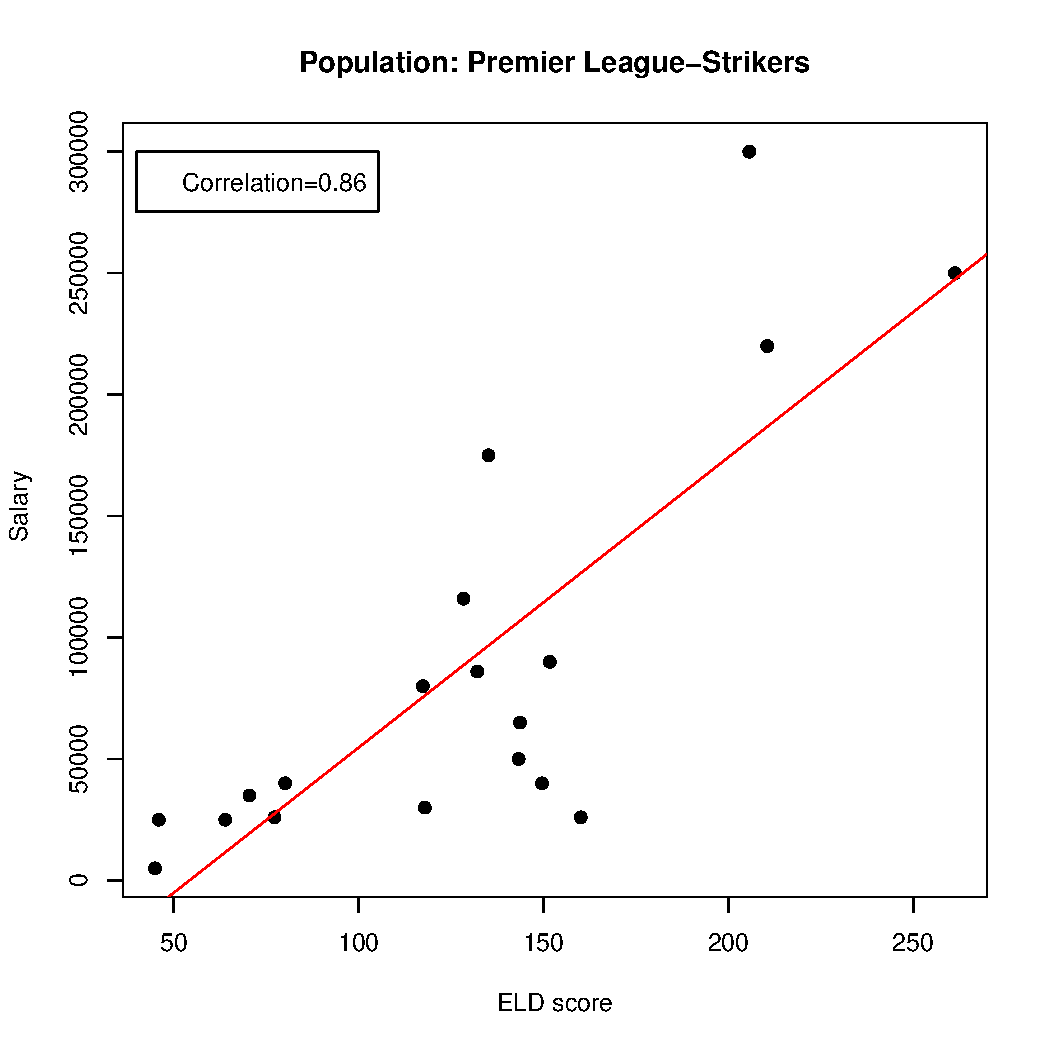
\includegraphics[width=2.5in]{NewPlotsJan2016/1d-sumStrikerSalary.pdf}
%			\caption{Strikers: Salary vs ELD. \textbf{How many strikers?}}
%			\label{fig:StrikerSalary}
%		\end{minipage}
%		\hspace{0.05\linewidth}
%		\begin{minipage}{0.45\linewidth}
%			\centering
%			\includegraphics[width=2.5in]{NewPlotsJan2016/1d-ShotsonTarget-sumStrikerStatistics.pdf}
%			\caption{Strikers: Shots On Target vs ELD}
%			\label{fig:StrikerShot}
%		\end{minipage}
%		\hspace{0.05\linewidth}
%		\begin{minipage}{0.45\linewidth}
%			\centering
%			\includegraphics[width=2.5in]{NewPlotsJan2016/1d-sumStrikerStatistics.pdf}
%			\caption{Strikers: Time played vs ELD. \textbf{Why strikers only?}}
%			\label{fig:StrikerTime}
%		\end{minipage}
%	\end{figure}

% Non-BibTeX users please use
%\begin{thebibliography}{}
%%
%% and use \bibitem to create references. Consult the Instructions
%% for authors for reference list style.
%%
%\bibitem{RefJ}
%% Format for Journal Reference
%Author, Article title, Journal, Volume, page numbers (year)
%% Format for books
%\bibitem{RefB}
%Author, Book title, page numbers. Publisher, place (year)
%% etc
%\end{thebibliography}

%\subsubsection{Goalie Success} 





	


%\begin{figure} \label{fig:goalies}
%		\centering
%%		\begin{minipage}{0.45\linewidth}
%%			\centering
%%			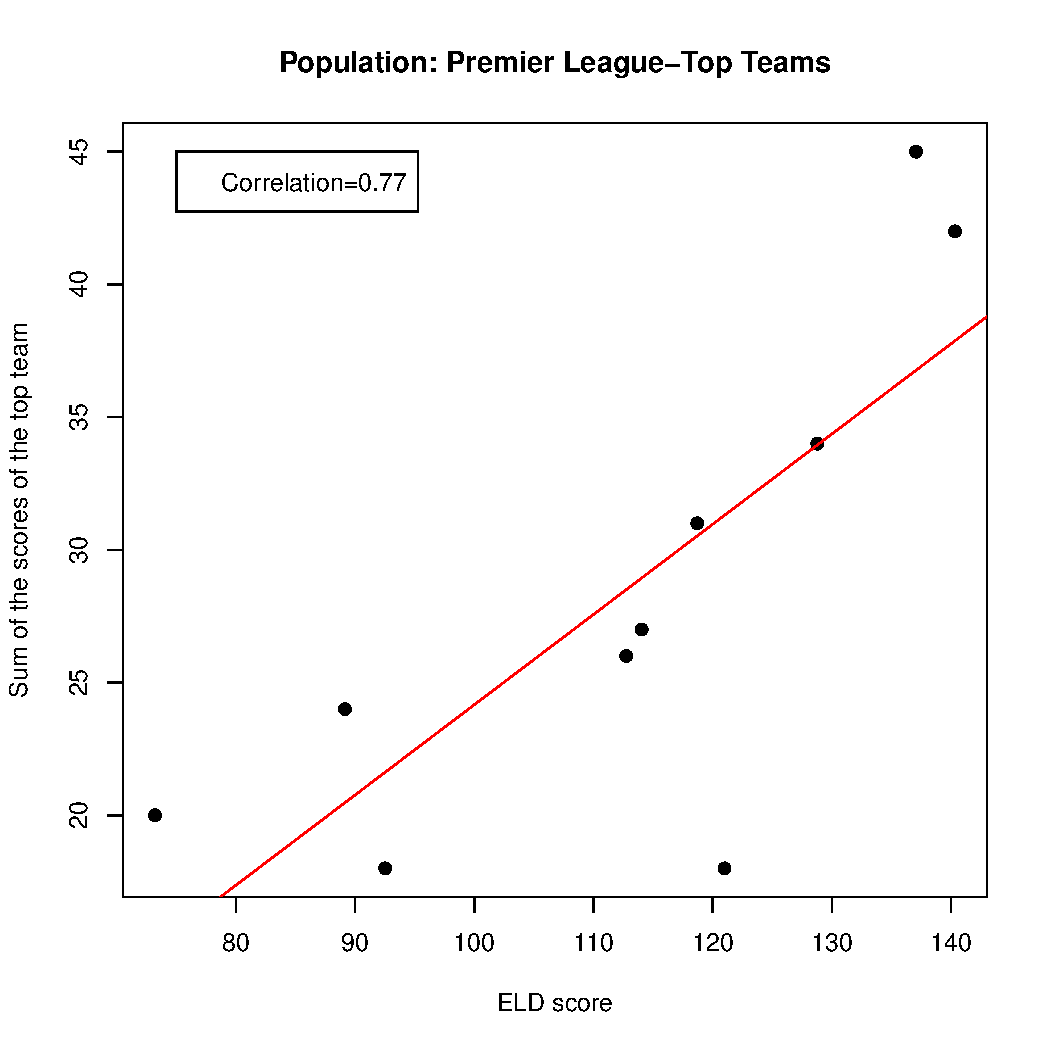
\includegraphics[width=2.5in]{NewPlotsJan2016/topTeamStats.pdf}
%%			\caption{Teams: Correlation between team's Standing and ELD for the top teams in Premier League standing}
%%			\label{fig:teamStanding}
%%		\end{minipage}
%%		\hspace{0.05\linewidth}
%		\begin{minipage}{0.45\linewidth}
%			\centering
%			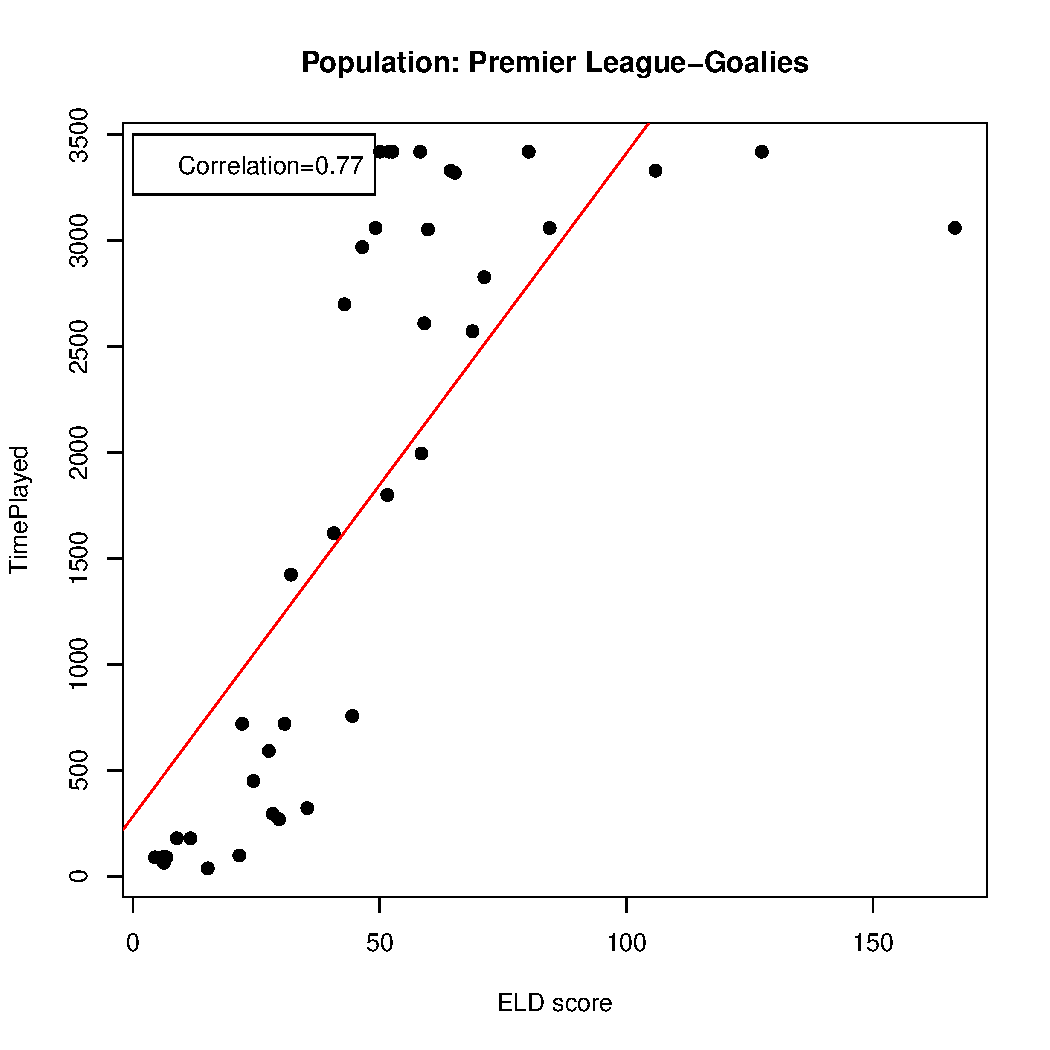
\includegraphics[width=2.5in]{NewPlotsJan2016/sumGoalieStatistics.pdf}
%			\caption{Goalies: sum of time played vs ELD}
%			\label{fig:GoalieTime}
%		\end{minipage}
%		\hspace{0.05\linewidth}
%		\begin{minipage}{0.45\linewidth}
%			\centering
%			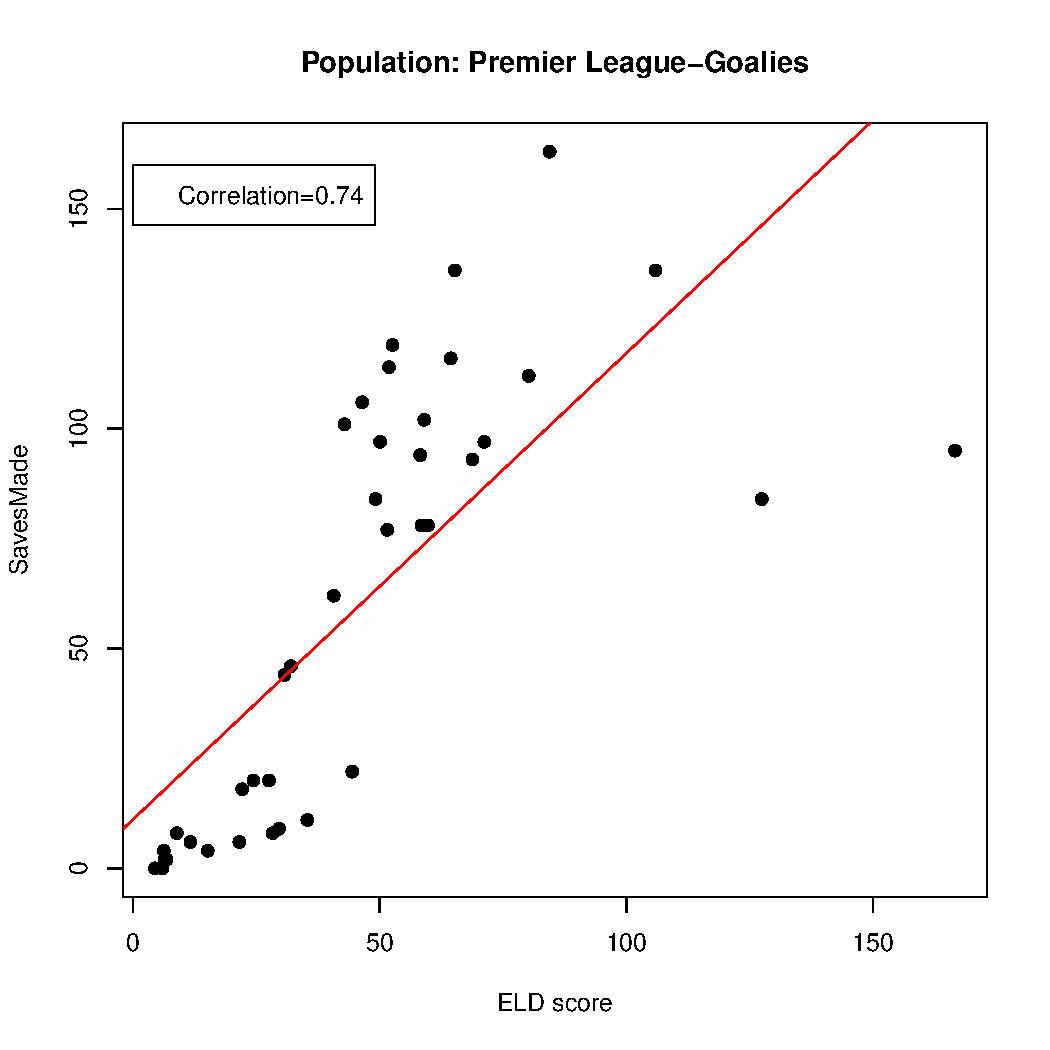
\includegraphics[width=2.5in]{NewPlotsJan2016/sumGoalieStatisticsSavesMade.pdf}
%			\caption{Goalies: sum of saves made vs ELD}
%			\label{fig:GoalieSaves}
%		\end{minipage}
%	\end{figure}



%
%Figure~\ref{fig:teamStanding} shows the scatter plot of this correlation and its best fit regression line.

%\begin{figure} \label{fig:teamStanding}
%		\centering
%		\begin{minipage}{0.45\linewidth}
%			\centering
%			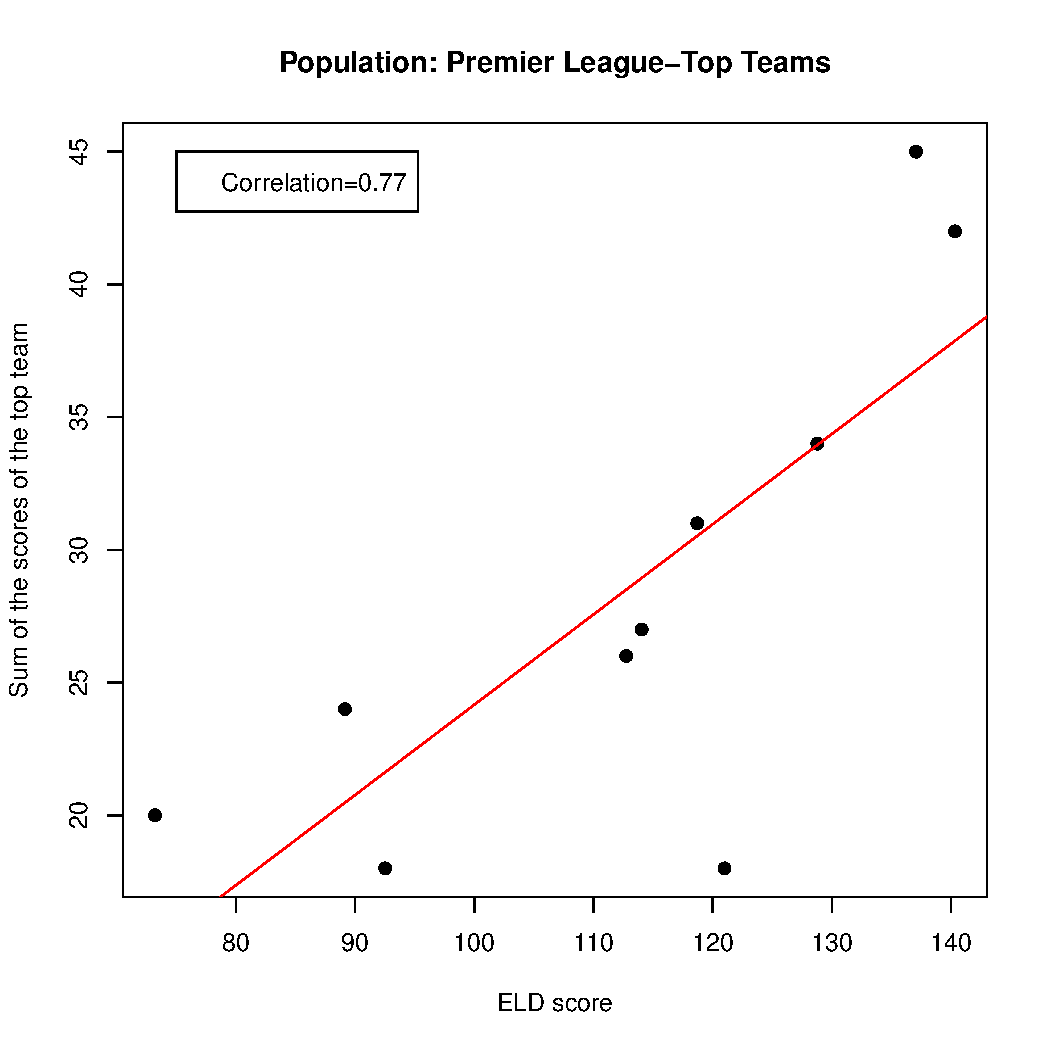
\includegraphics[width=2.5in]{NewPlotsJan2016/topTeamStats.pdf}
%			\caption{Teams: Correlation between team's Standing and ELD for the top teams in Premier League standing}
%			\label{fig:teamStanding}
%		\end{minipage}
%	\end{figure}


%\subsubsection{Movie Success} 




%\begin{figure} \label{fig:Movies}
%		\centering
%		\begin{minipage}{0.465\linewidth}
%			\centering
%			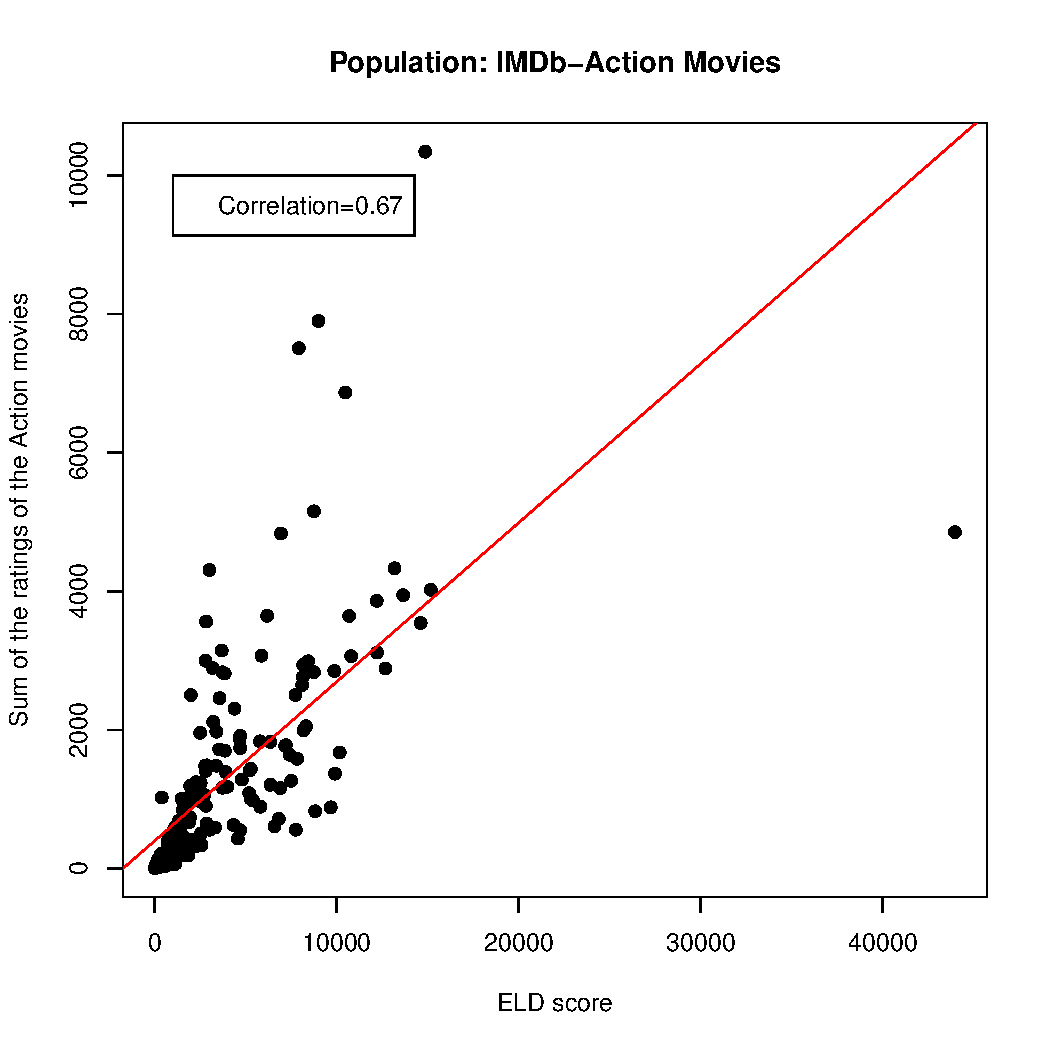
\includegraphics[width=2.5in]{NewPlotsJan2016/Action-Correlation.pdf}
%			\caption{Action movies: sum of ratings by users vs ELD}
%			\label{fig:ActionRate}
%		\end{minipage}
%		\hspace{0.05\linewidth}
%		\begin{minipage}{0.465\linewidth}
%			\centering
%			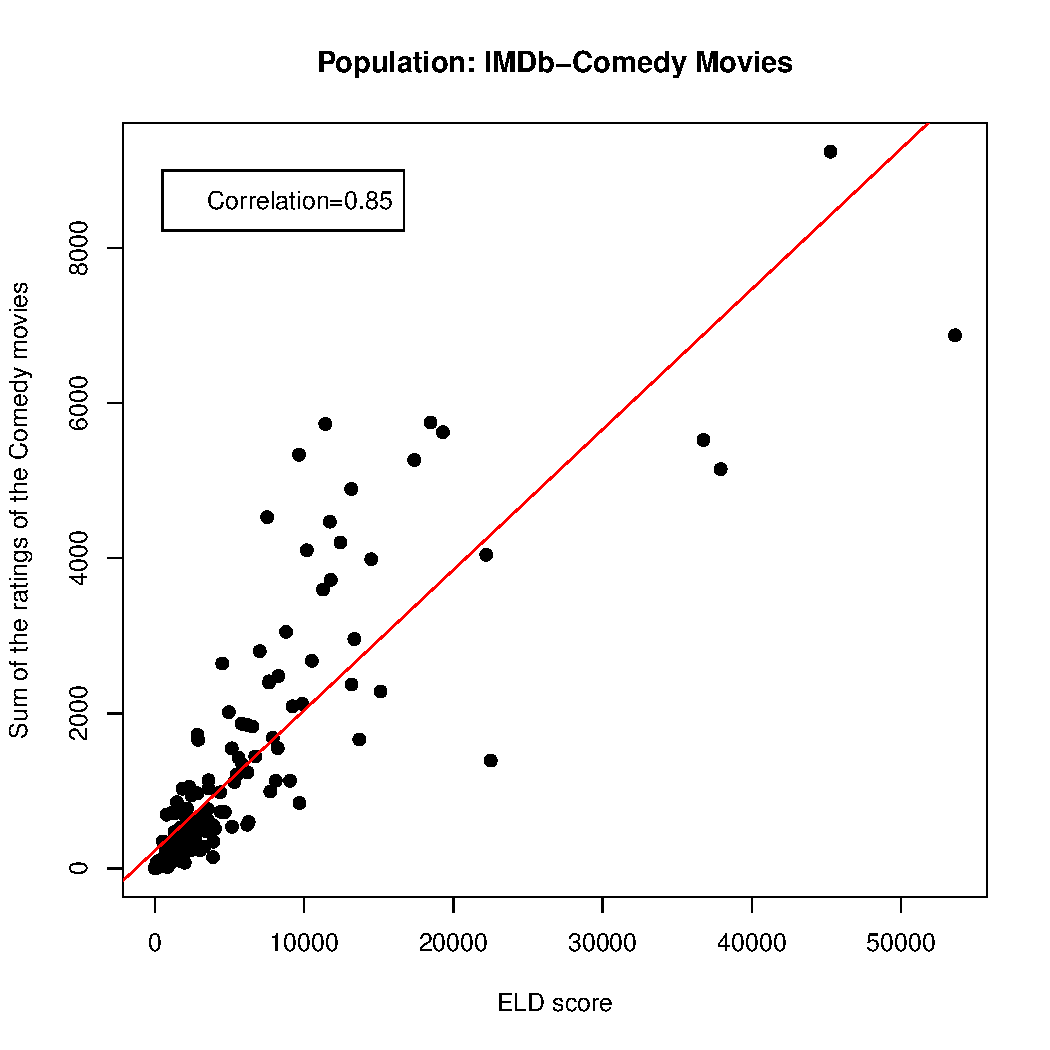
\includegraphics[width=2.5in]{NewPlotsJan2016/Comedy-Correlation.pdf}
%			\caption{Comedy movies: sum of ratings by users vs ELD}
%			\label{fig:ComedyRate}
%		\end{minipage}
%		\hspace{0.05\linewidth}
%		\begin{minipage}{0.465\linewidth}
%			\centering
%			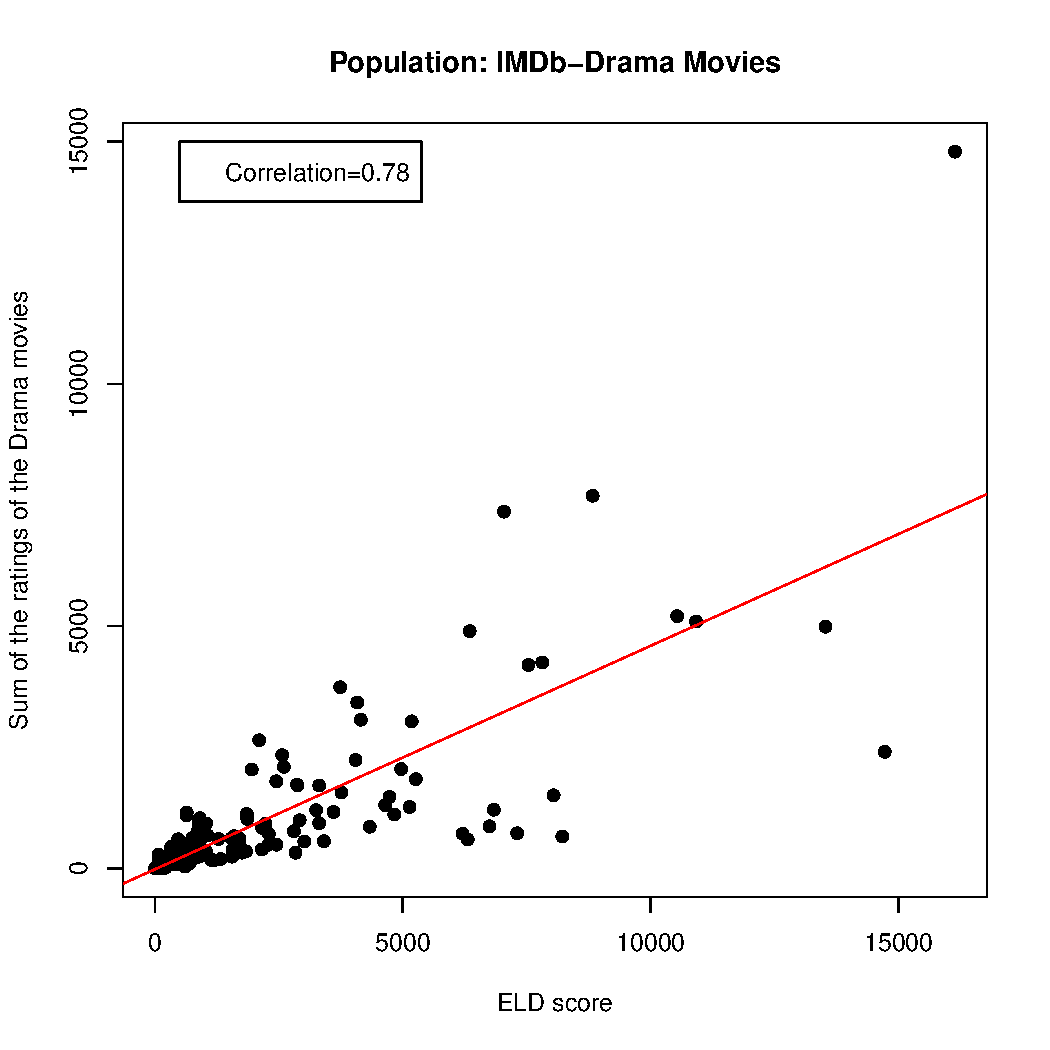
\includegraphics[width=2.5in]{NewPlotsJan2016/Drama-Correlation.pdf}
%			\caption{Drama movies: sum of ratings by users vs ELD \textbf{Average Rating?}}
%			\label{fig:DramaRate}
%		\end{minipage}
%	\end{figure}
%	
\bibliographystyle {plainnat}
\bibliography{\jobname} 
%\bibliography{dami} 
\end{document}
